\documentclass{article}

% TODO : CLEAN UP THIS MESS
% (AND MAKE SURE ALL TEXTS STILL COMPILE)
\usepackage[leqno]{amsmath}
\usepackage{amssymb}
\usepackage{graphicx}

\usepackage{diagbox} % table heads with diagonal lines
\usepackage{relsize}

\usepackage{wasysym}
\usepackage{scrextend}
\usepackage{epigraph}
\setlength\epigraphwidth{.6\textwidth}

\usepackage[utf8]{inputenc}

\usepackage{titlesec}
\titleformat{\chapter}[display]
  {\normalfont\sffamily\huge\bfseries}
  {\chaptertitlename\ \thechapter}{5pt}{\Huge}
\titleformat{\section}
  {\normalfont\sffamily\Large\bfseries}
  {\thesection}{1em}{}
\titleformat{\subsection}
  {\normalfont\sffamily\large\bfseries}
  {\thesubsection}{1em}{}
\titleformat{\part}[display]
  {\normalfont\sffamily\huge\bfseries}
  {\partname\ \thepart}{0pt}{\Huge}

\usepackage[T1]{fontenc}
\usepackage{fourier}
\usepackage{paratype}

\usepackage[symbol,perpage]{footmisc}

\usepackage{perpage}
\MakePerPage{footnote}

\usepackage{array}
\newcolumntype{x}[1]{>{\centering\hspace{0pt}}p{#1}}

% TODO: the following line causes conflict with new texlive (!)
% \usepackage[english,russian,polutonikogreek,spanish]{babel}
% \newcommand{\russian}[1]{{\selectlanguage{russian}#1}}

% Remove conflicting options for the moment:
\usepackage[english,polutonikogreek,spanish]{babel}

\AtBeginDocument{\shorthandoff{"}}
\newcommand{\greek}[1]{{\selectlanguage{polutonikogreek}#1}}

% % % % % % % % % % % % % % % % % % % % % % % % % % % % % %
% Limit/colimit symbols (with accented i: lím / colím)

\usepackage{etoolbox} % \patchcmd

\makeatletter
\patchcmd{\varlim@}{lim}{\lim}{}{}
\makeatother
\DeclareMathOperator*{\colim}{co{\lim}}
\newcommand{\dirlim}{\varinjlim}
\newcommand{\invlim}{\varprojlim}

% % % % % % % % % % % % % % % % % % % % % % % % % % % % % %

\usepackage[all,color]{xy}

\usepackage{pigpen}
\newcommand{\po}{\ar@{}[dr]|(.4){\text{\pigpenfont I}}}
\newcommand{\pb}{\ar@{}[dr]|(.3){\text{\pigpenfont A}}}
\newcommand{\polr}{\ar@{}[dr]|(.65){\text{\pigpenfont A}}}
\newcommand{\pour}{\ar@{}[ur]|(.65){\text{\pigpenfont G}}}
\newcommand{\hstar}{\mathop{\bigstar}}

\newcommand{\bigast}{\mathop{\Huge \mathlarger{\mathlarger{\ast}}}}

\newcommand{\term}{\textbf}

\usepackage{stmaryrd}

\usepackage{cancel}

\usepackage{tikzsymbols}

\newcommand{\open}{\underset{\mathrm{open}}{\hookrightarrow}}
\newcommand{\closed}{\underset{\mathrm{closed}}{\hookrightarrow}}

\newcommand{\tcol}[2]{{#1 \choose #2}}

\newcommand{\homot}{\simeq}
\newcommand{\isom}{\cong}
\newcommand{\cH}{\mathcal{H}}
\renewcommand{\hom}{\mathrm{hom}}
\renewcommand{\div}{\mathop{\mathrm{div}}}
\renewcommand{\Im}{\mathop{\mathrm{Im}}}
\renewcommand{\Re}{\mathop{\mathrm{Re}}}
\newcommand{\id}[1]{\mathrm{id}_{#1}}
\newcommand{\idid}{\mathrm{id}}

\newcommand{\ZG}{{\ZZ G}}
\newcommand{\ZH}{{\ZZ H}}

\newcommand{\quiso}{\simeq}

\newcommand{\personality}[1]{{\sc #1}}

\newcommand{\mono}{\rightarrowtail}
\newcommand{\epi}{\twoheadrightarrow}
\newcommand{\xepi}[1]{\xrightarrow{#1}\mathrel{\mkern-14mu}\rightarrow}

% % % % % % % % % % % % % % % % % % % % % % % % % % % % % %

\DeclareMathOperator{\Ad}{Ad}
\DeclareMathOperator{\Aff}{Aff}
\DeclareMathOperator{\Ann}{Ann}
\DeclareMathOperator{\Aut}{Aut}
\DeclareMathOperator{\Br}{Br}
\DeclareMathOperator{\CH}{CH}
\DeclareMathOperator{\Cl}{Cl}
\DeclareMathOperator{\Coeq}{Coeq}
\DeclareMathOperator{\Coind}{Coind}
\DeclareMathOperator{\Cop}{Cop}
\DeclareMathOperator{\Corr}{Corr}
\DeclareMathOperator{\Cor}{Cor}
\DeclareMathOperator{\Cov}{Cov}
\DeclareMathOperator{\Der}{Der}
\DeclareMathOperator{\Div}{Div}
\DeclareMathOperator{\D}{D}
\DeclareMathOperator{\Ehr}{Ehr}
\DeclareMathOperator{\End}{End}
\DeclareMathOperator{\Eq}{Eq}
\DeclareMathOperator{\Ext}{Ext}
\DeclareMathOperator{\Frac}{Frac}
\DeclareMathOperator{\Frob}{Frob}
\DeclareMathOperator{\Funct}{Funct}
\DeclareMathOperator{\Fun}{Fun}
\DeclareMathOperator{\GL}{GL}
\DeclareMathOperator{\Gal}{Gal}
\DeclareMathOperator{\Gr}{Gr}
\DeclareMathOperator{\Hol}{Hol}
\DeclareMathOperator{\Hom}{Hom}
\DeclareMathOperator{\Ho}{Ho}
\DeclareMathOperator{\Id}{Id}
\DeclareMathOperator{\Ind}{Ind}
\DeclareMathOperator{\Inn}{Inn}
\DeclareMathOperator{\Isom}{Isom}
\DeclareMathOperator{\Ker}{Ker}
\DeclareMathOperator{\Lan}{Lan}
\DeclareMathOperator{\Lie}{Lie}
\DeclareMathOperator{\Map}{Map}
\DeclareMathOperator{\Mat}{Mat}
\DeclareMathOperator{\Max}{Max}
\DeclareMathOperator{\Mor}{Mor}
\DeclareMathOperator{\Nat}{Nat}
\DeclareMathOperator{\Nrd}{Nrd}
\DeclareMathOperator{\Ob}{Ob}
\DeclareMathOperator{\Out}{Out}
\DeclareMathOperator{\PGL}{PGL}
\DeclareMathOperator{\PSL}{PSL}
\DeclareMathOperator{\PSU}{PSU}
\DeclareMathOperator{\Pic}{Pic}
\DeclareMathOperator{\RHom}{RHom}
\DeclareMathOperator{\Rad}{Rad}
\DeclareMathOperator{\Ran}{Ran}
\DeclareMathOperator{\Rep}{Rep}
\DeclareMathOperator{\Res}{Res}
\DeclareMathOperator{\SL}{SL}
\DeclareMathOperator{\SO}{SO}
\DeclareMathOperator{\SU}{SU}
\DeclareMathOperator{\Sh}{Sh}
\DeclareMathOperator{\Sing}{Sing}
\DeclareMathOperator{\Specm}{Specm}
\DeclareMathOperator{\Spec}{Spec}
\DeclareMathOperator{\Sp}{Sp}
\DeclareMathOperator{\Stab}{Stab}
\DeclareMathOperator{\Sym}{Sym}
\DeclareMathOperator{\Tors}{Tors}
\DeclareMathOperator{\Tor}{Tor}
\DeclareMathOperator{\Tot}{Tot}
\DeclareMathOperator{\UUU}{U}

\DeclareMathOperator{\adj}{adj}
\DeclareMathOperator{\ad}{ad}
\DeclareMathOperator{\af}{af}
\DeclareMathOperator{\card}{card}
\DeclareMathOperator{\cm}{cm}
\DeclareMathOperator{\codim}{codim}
\DeclareMathOperator{\cod}{cod}
\DeclareMathOperator{\coeq}{coeq}
\DeclareMathOperator{\coim}{coim}
\DeclareMathOperator{\coker}{coker}
\DeclareMathOperator{\cont}{cont}
\DeclareMathOperator{\conv}{conv}
\DeclareMathOperator{\cor}{cor}
\DeclareMathOperator{\depth}{depth}
\DeclareMathOperator{\diag}{diag}
\DeclareMathOperator{\diam}{diam}
\DeclareMathOperator{\dist}{dist}
\DeclareMathOperator{\dom}{dom}
\DeclareMathOperator{\eq}{eq}
\DeclareMathOperator{\ev}{ev}
\DeclareMathOperator{\ex}{ex}
\DeclareMathOperator{\fchar}{char}
\DeclareMathOperator{\fr}{fr}
\DeclareMathOperator{\gr}{gr}
\DeclareMathOperator{\im}{im}
\DeclareMathOperator{\infl}{inf}
\DeclareMathOperator{\interior}{int}
\DeclareMathOperator{\intrel}{intrel}
\DeclareMathOperator{\inv}{inv}
\DeclareMathOperator{\length}{length}
\DeclareMathOperator{\mcd}{mcd}
\DeclareMathOperator{\mcm}{mcm}
\DeclareMathOperator{\multideg}{multideg}
\DeclareMathOperator{\ord}{ord}
\DeclareMathOperator{\pr}{pr}
\DeclareMathOperator{\rel}{rel}
\DeclareMathOperator{\res}{res}
\DeclareMathOperator{\rkred}{rkred}
\DeclareMathOperator{\rkss}{rkss}
\DeclareMathOperator{\rk}{rk}
\DeclareMathOperator{\sgn}{sgn}
\DeclareMathOperator{\sk}{sk}
\DeclareMathOperator{\supp}{supp}
\DeclareMathOperator{\trdeg}{trdeg}
\DeclareMathOperator{\tr}{tr}
\DeclareMathOperator{\vol}{vol}

\newcommand{\iHom}{\underline{\Hom}}

\renewcommand{\AA}{\mathbb{A}}
\newcommand{\CC}{\mathbb{C}}
\renewcommand{\SS}{\mathbb{S}}
\newcommand{\TT}{\mathbb{T}}
\newcommand{\PP}{\mathbb{P}}
\newcommand{\BB}{\mathbb{B}}
\newcommand{\RR}{\mathbb{R}}
\newcommand{\ZZ}{\mathbb{Z}}
\newcommand{\FF}{\mathbb{F}}
\newcommand{\HH}{\mathbb{H}}
\newcommand{\NN}{\mathbb{N}}
\newcommand{\QQ}{\mathbb{Q}}
\newcommand{\KK}{\mathbb{K}}

% % % % % % % % % % % % % % % % % % % % % % % % % % % % % %

\usepackage{amsthm}

\newcommand{\legendre}[2]{\left(\frac{#1}{#2}\right)}

\newcommand{\examplesymbol}{$\blacktriangle$}
\renewcommand{\qedsymbol}{$\blacksquare$}

\newcommand{\dfn}{\mathrel{\mathop:}=}
\newcommand{\rdfn}{=\mathrel{\mathop:}}

\usepackage{xcolor}
\definecolor{mylinkcolor}{rgb}{0.0,0.4,1.0}
\definecolor{mycitecolor}{rgb}{0.0,0.4,1.0}
\definecolor{shadecolor}{rgb}{0.79,0.78,0.65}
\definecolor{gray}{rgb}{0.6,0.6,0.6}

\usepackage{colortbl}

\definecolor{myred}{rgb}{0.7,0.0,0.0}
\definecolor{mygreen}{rgb}{0.0,0.7,0.0}
\definecolor{myblue}{rgb}{0.0,0.0,0.7}

\definecolor{redshade}{rgb}{0.9,0.5,0.5}
\definecolor{greenshade}{rgb}{0.5,0.9,0.5}

\usepackage[unicode,colorlinks=true,linkcolor=mylinkcolor,citecolor=mycitecolor]{hyperref}
\newcommand{\refref}[2]{\hyperref[#2]{#1~\ref*{#2}}}
\newcommand{\eqnref}[1]{\hyperref[#1]{(\ref*{#1})}}

\newcommand{\tos}{\!\!\to\!\!}

\usepackage{framed}

\newcommand{\cequiv}{\simeq}

\makeatletter
\newcommand\xleftrightarrow[2][]{%
  \ext@arrow 9999{\longleftrightarrowfill@}{#1}{#2}}
\newcommand\longleftrightarrowfill@{%
  \arrowfill@\leftarrow\relbar\rightarrow}
\makeatother

\newcommand{\bsquare}{\textrm{\ding{114}}}

% % % % % % % % % % % % % % % % % % % % % % % % % % % % % %

\newtheoremstyle{myplain}
  {\topsep}   % ABOVESPACE
  {\topsep}   % BELOWSPACE
  {\itshape}  % BODYFONT
  {0pt}       % INDENT (empty value is the same as 0pt)
  {\bfseries} % HEADFONT
  {.}         % HEADPUNCT
  {5pt plus 1pt minus 1pt} % HEADSPACE
  {\thmnumber{#2}. \thmname{#1}\thmnote{ (#3)}}   % CUSTOM-HEAD-SPEC

\newtheoremstyle{myplainnameless}
  {\topsep}   % ABOVESPACE
  {\topsep}   % BELOWSPACE
  {\normalfont}  % BODYFONT
  {0pt}       % INDENT (empty value is the same as 0pt)
  {\bfseries} % HEADFONT
  {.}         % HEADPUNCT
  {5pt plus 1pt minus 1pt} % HEADSPACE
  {\thmnumber{#2}}   % CUSTOM-HEAD-SPEC 

\newtheoremstyle{sectionexercise}
  {\topsep}   % ABOVESPACE
  {\topsep}   % BELOWSPACE
  {\normalfont}  % BODYFONT
  {0pt}       % INDENT (empty value is the same as 0pt)
  {\bfseries} % HEADFONT
  {.}         % HEADPUNCT
  {5pt plus 1pt minus 1pt} % HEADSPACE
  {Ejercicio \thmnumber{#2}\thmnote{ (#3)}}   % CUSTOM-HEAD-SPEC

\newtheoremstyle{mydefinition}
  {\topsep}   % ABOVESPACE
  {\topsep}   % BELOWSPACE
  {\normalfont}  % BODYFONT
  {0pt}       % INDENT (empty value is the same as 0pt)
  {\bfseries} % HEADFONT
  {.}         % HEADPUNCT
  {5pt plus 1pt minus 1pt} % HEADSPACE
  {\thmnumber{#2}. \thmname{#1}\thmnote{ (#3)}}   % CUSTOM-HEAD-SPEC

% EN ESPAÑOL

\newtheorem*{hecho*}{Hecho}
\newtheorem*{corolario*}{Corolario}
\newtheorem*{teorema*}{Teorema}
\newtheorem*{conjetura*}{Conjetura}
\newtheorem*{proyecto*}{Proyecto}
\newtheorem*{observacion*}{Observación}

\newtheorem*{lema*}{Lema}
\newtheorem*{resultado-clave*}{Resultado clave}
\newtheorem*{proposicion*}{Proposición}

\theoremstyle{definition}
\newtheorem*{ejercicio*}{Ejercicio}
\newtheorem*{definicion*}{Definición}
\newtheorem*{comentario*}{Comentario}
\newtheorem*{definicion-alternativa*}{Definición alternativa}
\newtheorem*{ejemploxs}{Ejemplo}
\newenvironment{ejemplo*}
  {\pushQED{\qed}\renewcommand{\qedsymbol}{\examplesymbol}\ejemploxs}
  {\popQED\endejemploxs}

\theoremstyle{myplain}
\newtheorem{proposicion}{Proposición}[section]

\newtheorem{proyecto}[proposicion]{Proyecto}
\newtheorem{teorema}[proposicion]{Teorema}
\newtheorem{corolario}[proposicion]{Corolario}
\newtheorem{hecho}[proposicion]{Hecho}
\newtheorem{lema}[proposicion]{Lema}

\newtheorem{observacion}[proposicion]{Observación}

\newenvironment{observacionejerc}
    {\pushQED{\qed}\renewcommand{\qedsymbol}{$\square$}\csname inner@observacionejerc\endcsname}
    {\popQED\csname endinner@observacionejerc\endcsname}
\newtheorem{inner@observacionejerc}[proposicion]{Observación}

\newenvironment{proposicionejerc}
    {\pushQED{\qed}\renewcommand{\qedsymbol}{$\square$}\csname inner@proposicionejerc\endcsname}
    {\popQED\csname endinner@proposicionejerc\endcsname}
\newtheorem{inner@proposicionejerc}[proposicion]{Proposicion}

\newenvironment{lemaejerc}
    {\pushQED{\qed}\renewcommand{\qedsymbol}{$\square$}\csname inner@lemaejerc\endcsname}
    {\popQED\csname endinner@lemaejerc\endcsname}
\newtheorem{inner@lemaejerc}[proposicion]{Lema}

\newtheorem{calculo}[proposicion]{Cálculo}

\theoremstyle{myplainnameless}
\newtheorem{nameless}[proposicion]{}

\theoremstyle{mydefinition}
\newtheorem{comentario}[proposicion]{Comentario}
\newtheorem{comentarioast}[proposicion]{Comentario ($\clubsuit$)}
\newtheorem{construccion}[proposicion]{Construcción}
\newtheorem{aplicacion}[proposicion]{Aplicación}
\newtheorem{definicion}[proposicion]{Definición}
\newtheorem{definicion-alternativa}[proposicion]{Definición alternativa}
\newtheorem{notacion}[proposicion]{Notación}
\newtheorem{advertencia}[proposicion]{Advertencia}
\newtheorem{digresion}[proposicion]{Digresión}
\newtheorem{ejemplox}[proposicion]{Ejemplo}
\newenvironment{ejemplo}
  {\pushQED{\qed}\renewcommand{\qedsymbol}{\examplesymbol}\ejemplox}
  {\popQED\endejemplox}
\newtheorem{contraejemplox}[proposicion]{Contraejemplo}
\newenvironment{contraejemplo}
  {\pushQED{\qed}\renewcommand{\qedsymbol}{\examplesymbol}\contraejemplox}
  {\popQED\endcontraejemplox}
\newtheorem{noejemplox}[proposicion]{No-ejemplo}
\newenvironment{noejemplo}
  {\pushQED{\qed}\renewcommand{\qedsymbol}{\examplesymbol}\noejemplox}
  {\popQED\endnoejemplox}
 
\newtheorem{ejemploastx}[proposicion]{Ejemplo ($\clubsuit$)}
\newenvironment{ejemploast}
  {\pushQED{\qed}\renewcommand{\qedsymbol}{\examplesymbol}\ejemploastx}
  {\popQED\endejemploastx}

\ifdefined\exercisespersection
  \theoremstyle{sectionexercise}
  \newtheorem{ejercicio}{}[section]
  \theoremstyle{mydefinition}
\else
  \ifdefined\exercisesglobal
    \theoremstyle{sectionexercise}
    \newtheorem{ejercicio}{}
    \theoremstyle{mydefinition}
  \else
    \ifdefined\exercisespersection
      \newtheorem{ejercicio}[proposicion]{Ejercicio}
    \fi
  \fi
\fi

% % % % % % % % % % % % % % % % % % % % % % % % % % % % % %

\theoremstyle{myplain}
\newtheorem{proposition}{Proposition}[section]
\newtheorem*{fact*}{Fact}
\newtheorem*{proposition*}{Proposition}
\newtheorem{lemma}[proposition]{Lemma}
\newtheorem*{lemma*}{Lemma}

\newtheorem{exercise}{Exercise}
\newtheorem*{hint}{Hint}

\newtheorem{theorem}[proposition]{Theorem}
\newtheorem{conjecture}[proposition]{Conjecture}
\newtheorem*{theorem*}{Theorem}
\newtheorem{corollary}[proposition]{Corollary}
\newtheorem{fact}[proposition]{Fact}
\newtheorem*{claim}{Claim}
\newtheorem{definition-theorem}[proposition]{Definition-theorem}

\theoremstyle{mydefinition}
\newtheorem{examplex}[proposition]{Example}
\newenvironment{example}
  {\pushQED{\qed}\renewcommand{\qedsymbol}{\examplesymbol}\examplex}
  {\popQED\endexamplex}

\newtheorem*{examplexx}{Example}
\newenvironment{example*}
  {\pushQED{\qed}\renewcommand{\qedsymbol}{\examplesymbol}\examplexx}
  {\popQED\endexamplexx}

\newtheorem{definition}[proposition]{Definition}
\newtheorem*{definition*}{Definition}
\newtheorem{wrong-definition}[proposition]{Wrong definition}
\newtheorem{remark}[proposition]{Remark}

\makeatletter
\newcommand{\xRightarrow}[2][]{\ext@arrow 0359\Rightarrowfill@{#1}{#2}}
\makeatother

% % % % % % % % % % % % % % % % % % % % % % % % % % % % % %

\newcommand{\Et}{\mathop{\text{\rm Ét}}}

\newcommand{\categ}[1]{\text{\bf #1}}
\newcommand{\vcateg}{\mathcal}
\newcommand{\bone}{{\boldsymbol 1}}
\newcommand{\bDelta}{{\boldsymbol\Delta}}
\newcommand{\bR}{{\mathbf{R}}}

\newcommand{\univ}{\mathfrak}

\newcommand{\TODO}{\colorbox{red}{\textbf{*** TODO ***}}}
\newcommand{\proofreadme}{\colorbox{red}{\textbf{*** NEEDS PROOFREADING ***}}}

\makeatletter
\def\iddots{\mathinner{\mkern1mu\raise\p@
\vbox{\kern7\p@\hbox{.}}\mkern2mu
\raise4\p@\hbox{.}\mkern2mu\raise7\p@\hbox{.}\mkern1mu}}
\makeatother

\newcommand{\ssincl}{\reflectbox{\rotatebox[origin=c]{45}{$\subseteq$}}}
\newcommand{\vsupseteq}{\reflectbox{\rotatebox[origin=c]{-90}{$\supseteq$}}}
\newcommand{\vin}{\reflectbox{\rotatebox[origin=c]{90}{$\in$}}}

\newcommand{\Ga}{\mathbb{G}_\mathrm{a}}
\newcommand{\Gm}{\mathbb{G}_\mathrm{m}}

\renewcommand{\U}{\UUU}

\DeclareRobustCommand{\Stirling}{\genfrac\{\}{0pt}{}}
\DeclareRobustCommand{\stirling}{\genfrac[]{0pt}{}}

% % % % % % % % % % % % % % % % % % % % % % % % % % % % % %
% tikz

\usepackage{tikz-cd}
\usetikzlibrary{babel}
\usetikzlibrary{decorations.pathmorphing}
\usetikzlibrary{arrows}
\usetikzlibrary{calc}
\usetikzlibrary{fit}
\usetikzlibrary{hobby}

% % % % % % % % % % % % % % % % % % % % % % % % % % % % % %
% Banners

\newcommand\mybannerext[3]{{\normalfont\sffamily\bfseries\large\noindent #1

\noindent #2

\noindent #3

}\noindent\rule{\textwidth}{1.25pt}

\vspace{1em}}

\newcommand\mybanner[2]{{\normalfont\sffamily\bfseries\large\noindent #1

\noindent #2

}\noindent\rule{\textwidth}{1.25pt}

\vspace{1em}}

\renewcommand{\O}{\mathcal{O}}


\numberwithin{equation}{section}

\newcounter{ejerctot}
\setcounter{ejerctot}{0}
\newcommand{\ejerccount}{\stepcounter{ejerctot}\theejerctot/68}

\usepackage[numbers]{natbib}

\usepackage{fullpage}

\usepackage{tocloft}

\renewcommand\cftsecfont{\normalfont}
\renewcommand\cfttoctitlefont{\sffamily\large\bfseries}
\renewcommand\cftsecpagefont{\normalfont}
\renewcommand{\cftsecleader}{\cftdotfill{\cftsecdotsep}}
\renewcommand\cftsecdotsep{\cftdot}
\renewcommand\cftsubsecdotsep{\cftdot}

\hypersetup{
  pdftitle = {Invitación a la teoría de esquemas},
  pdfauthor = {Alexey Beshenov (cadadr@gmail.com)},
  pdfdisplaydoctitle = true
}

\author{Alexey Beshenov (cadadr@gmail.com)}
\title{Invitación a la teoría de esquemas}
\date{Universidad de El Salvador. Agosto de 2019}

\usepackage{multicol}

\setlength{\columnseprule}{0.4pt}

\theoremstyle{definition}
\newtheorem{ejerc}{Ejercicio}[section]

\newif\ifsolutions
\solutionstrue
% \solutionsfalse

\usepackage{multirow}

\renewcommand*{\thefootnote}{\arabic{footnote})}

\begin{document}

{\normalfont\sffamily\bfseries \maketitle}

\epigraph{Recuerde: ¡Todo lo que sucede en matemáticas primero sucede
  en geometría algebraica!}{Oscar Zariski, citado por Gian-Carlo Rota}

\epigraph{\textbf{Pregunta del público}: ...si tratáramos de explicar a un lego
  qué es geometría algebraica, creo que todavía sería adecuado el título
  del viejo libro de Enriques ``Teoría geométrica de ecuaciones''.\\
  ¿Qué opina usted?

  \textbf{Grothendieck}: Sí, pero su ``lego'' debe saber qué es un sistema de
  ecuaciones algebraicas. Esto le costaría años de estudio a Platón.}{Apuntes de
  charlas de Grothendieck\\
  tomados por Federico Gaeta}

\epigraph{La idea de esquema surgió por primera vez en uno de
  [los seminarios de Cartan y Chevalley]. (Durante este seminario Grothendieck
  aparentemente preguntó: ``¿Qué es un esquema?'')}{\cite[Chapter
  6]{Scharlau-Spirituality}}

Estos apuntes corresponden a una serie de charlas que di en agosto de 2019 en
el programa de maestría en matemática fundamental de la Universidad de
El Salvador. El nombre oficial del minicurso era ``Introducción a la teoría
de esquemas'', pero es algo ambicioso y en realidad se trata de una
\emph{invitación} a la teoría. Mi objetivo era solamente explicar qué es
un esquema.

Asumo que el lector conozca un poco de álgebra conmutativa, topología general
y la teoría de categorías básica. Otros conceptos importantes, como la teoría
de haces, serán explicados brevemente en este texto.

La lectura adicional recomendada es \cite[Chapter I, II, VI]{Eisenbud-Harris},
\cite[Chapter 1--4]{Gortz-Wedhorn}, \cite[Chapter 5]{Shafarevich-BAG-2} y
\cite{Manin-Schemes}.

\subsection*{Historia de esquemas}

Técnicamente hablando, la noción de esquema no pertenece a nadie y nació en
los círculos de matemáticos parisinos en los años 50. Sin embargo,
fue \personality{Alexander Grothendieck} (1928--2014) quien desarrollo
sistemáticamente la \emph{teoría de esquemas}. Sus fundaciones se encuentran
en el tratado ``Éléments de géométrie algébrique'' escrito junto con
\personality{Jean Dieudonné} (1906--1992). Su primer volumen \cite{EGAI-new}
es muy relevante para nuestro minicurso, pero no es la mejor fuente para
empezar. El título es una referencia a los ``Elementos'' de Euclides. Sin duda,
Grothendieck, como Euclides, fue uno de los matemáticos más importantes
e influyentes de toda la historia de la humanidad. Para saber más de su vida
y filosofía, se puede consultar la página
\url{http://www.grothendieckcircle.org/} Además, Grothendieck escibió una larga
y controvertida autobiografía \cite{ReS}.

\begin{center}
  \noindent 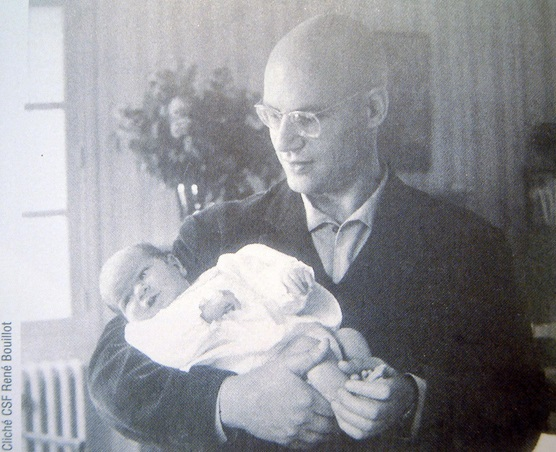
\includegraphics[width=8cm]{grothendieck.jpg}

  \vspace{1em}

  \noindent Alexander Grothendieck
\end{center}

Muchos textos importantes sobre la geometría algebraica grothendieckiana todavía
existen solamente en francés. Una fundación moderna de la teoría de esquemas
en inglés se encuentra en el \emph{Stacks project}:
\url{http://stacks.math.columbia.edu/}

\subsection*{Agradecimientos}

Agradezco a todos mis alumnos y colegas de El~Salvador que asistieron a mis
charlas: Francisco, Gabriel, Jorge, Mario, Mynor, y Yoceman.

\pagebreak

{\small\tableofcontents}

\pagebreak

% % % % % % % % % % % % % % % % % % % % % % % % % % % % % %

\section{El espectro como un espacio topológico}

\marginpar{\footnotesize sesión 1\\12/08/19}

Todos los anillos serán conmutativos con identidad. Un homomorfismo de anillos
$\phi\colon A\to B$ por la definición cumple $\phi (1_A) = 1_B$. La categoría
de anillos (conmutativos) será denotada por $\categ{CRing}$.

\subsection{Conjuntos cerrados $V (\mathfrak{a})$ y la topología de Zariski}

\begin{definicion}
  \label{dfn:Spec}
  El \term{espectro} de un anillo $A$ es el conjunto de sus ideales primos:
  \[ \Spec A \dfn \{ \mathfrak{p} \subset A \mid
                     \mathfrak{p}\text{ un ideal primo} \}. \]
\end{definicion}

Por el lema de Zorn, en todo anillo no nulo existe un ideal maximal, y por ende
${\Spec A \ne \emptyset}$, si $A \ne 0$.

\begin{digresion}
  \label{comentario:evaluacion-en-Spec}
  Recordemos que la topología de Zariski sobre el espacio afín $\AA^n (k)$ tiene
  como sus subconjuntos cerrados
  $$V (S) \dfn \{ x \in \AA^n (k) \mid f (x) = 0 \text{ para todo }f\in S \},$$
  donde $S \subseteq k [x_1,\ldots,x_n]$ es algún conjunto de polinomios.
  Nos gustaría definir una topología parecida sobre $\Spec A$. En este caso
  los puntos $x \in \Spec A$ son ideales primos $\mathfrak{p}_x \subset A$,
  y el rol de funciones que se evalúan en los puntos van a jugar los elementos
  de anillo $f \in A$. Esta evaluación $f (x)$ se define de manera formal como
  la imagen de $f$ en el cuerpo $\Frac (A/\mathfrak{p}_x)$:

  \[ \begin{tikzcd}[row sep=0pt]
      A \ar[->>]{r} & A/\mathfrak{p}_x \ar[hookrightarrow]{r} & \Frac (A/\mathfrak{p}_x) \\
      f \ar[|->]{r} & \overline{f} \ar[|->]{r} & f (x) \dfn \frac{\overline{f}}{1}
    \end{tikzcd} \]

  En este sentido los elementos de $A$ son funciones sobre $\Spec A$, aunque
  los valores de $f$ en diferentes puntos están en diferentes cuerpos. Notamos
  que bajo esta interpretación, $f (x) = 0$ si y solamente si
  $f \in \mathfrak{p}_x$. Todo esto motiva la siguiente definición.
\end{digresion}

\begin{definicion}
  \label{dfn:cerrados-V}
  Para un subconjunto $S \subseteq A$, pongamos
  $$V (S) \dfn \{ \mathfrak{p} \in \Spec A \mid \mathfrak{p} \supseteq S \}.$$
\end{definicion}

Cuando $S$ consiste en un elemento $f \in A$, vamos a escribir ``$V (f)$''
en lugar de ``$V (\{ f \})$''.

Notamos que si $\mathfrak{a} = (S)$ es el ideal en $A$ generado por $S$,
entonces $V (S) = V (\mathfrak{a})$ (se tiene $\mathfrak{p} \supseteq S$
si y solamente si $\mathfrak{p} \supseteq (S)$, puesto que $\mathfrak{p}$ es
un ideal).

\begin{observacion}
  Los conjuntos $V (S)$ tienen las siguientes propiedades.

  \begin{enumerate}
  \item[0)] Si $S \subseteq S'$, entonces $V (S) \supseteq V (S')$.

  \item[1)] $V (0) = \Spec A$ y $V (1) = \emptyset$.

  \item[2)] Para una familia de ideales $\mathfrak{a}_i \subseteq A$ se tiene
    $$V \Bigl(\bigcup_i \mathfrak{a}_i\Bigr) = V \Bigl(\sum_i \mathfrak{a}_i\Bigr) = \bigcap_i V (\mathfrak{a}_i).$$

  \item[3)] $V (\mathfrak{a} \cap \mathfrak{b}) = V (\mathfrak{ab}) = V (\mathfrak{a}) \cup V (\mathfrak{b})$.

  \item[4)] $V (\mathfrak{a}) = V (\sqrt{\mathfrak{a}})$.
  \end{enumerate}

  \begin{proof}
    Se sigue fácilmente de las definiciones. Para verificar 3), recuerde que si
    $\mathfrak{p}$ es un ideal primo, entonces
    \[ \mathfrak{p}\supseteq\mathfrak{a} \cap \mathfrak{b} \iff
       \mathfrak{p}\supseteq\mathfrak{ab} \iff
       \mathfrak{p}\supseteq\mathfrak{a}
       \text{ o }\mathfrak{p}\supseteq\mathfrak{b}. \]
    En 4), recordemos que todo ideal primo es radical, así que
    $\mathfrak{p} \supseteq \mathfrak{a}$ si y solamente si
    $\mathfrak{p} \supseteq \sqrt{\mathfrak{a}}$.
  \end{proof}
\end{observacion}

Las propiedades 1)--3) de arriba significan que los $V (\mathfrak{a})$
satisfacen los axiomas de conjuntos cerrados de una topología.

\begin{definicion}
  La topología sobre $\Spec A$ que tiene como conjuntos cerrados
  $V (\mathfrak{a})$ para ideales $\mathfrak{a} \subseteq A$ se llama
  la \term{topología de Zariski}.
\end{definicion}

A partir de ahora $\Spec A$ será considerado como un espacio topológico.

\subsection{Ideales $I (Y) \subseteq A$}

Recordemos que a un subconjunto $Y \subseteq \AA^n (k)$ se puede asignar
el ideal de polinomios que se anulan en los puntos de $Y$:
$$I (Y) = \{ f \in k [x_1,\ldots,x_n] \mid f (y) = 0 \text{ para todo }y\in Y \}.$$
Siguiendo la analogía explicada en \ref{comentario:evaluacion-en-Spec}, tiene
sentido considerar para $Y \subseteq \Spec A$
\[ I (Y) = \{ f \in A \mid f (y) = 0\text{ para todo }y\in Y \} =
   \{ f \in A \mid f\in\mathfrak{p}_y\text{ para todo }\mathfrak{p}_y\in Y \}. \]
Esto nos lleva a la siguiente definición.

\begin{definicion}
  \label{dfn:ideal-I}
  Dado un subconjunto $Y \subseteq \Spec A$, pongamos
  $$I (Y) \dfn \bigcap_{\mathfrak{p} \in Y} \mathfrak{p}.$$
\end{definicion}

En particular, $I (\emptyset) = A$ e $I (\Spec A) = N (A)$ es el nilradical
(la intersección de todos los ideales primos).

\begin{observacion}
  Los ideales $I (Y) \subseteq A$ tienen las siguientes propiedades.

  \begin{enumerate}
  \item[0)] Si $Y \subseteq Y'$, entonces $I (Y) \supseteq I (Y')$.

  \item[1)] $IV (\mathfrak{a}) = \sqrt{a}$.

  \item[2)] $I (Y)$ es un ideal radical; es decir, $\sqrt{I (Y)} = I (Y)$.

  \item[3)] $VI (Y) = \overline{Y}$ es la clausura de $Y$ respecto a
    la topología de Zariski.
  \end{enumerate}

  \begin{proof}
    La parte 0) está clara de la definición. En la parte 1), recordemos que
    \[ \sqrt{\mathfrak{a}} =
       \bigcap_{\substack{\mathfrak{p} \in \Spec A \\ \mathfrak{p}\supseteq\mathfrak{a}}} \mathfrak{p}, \]
    pero esta intersección es exactamente $IV (\mathfrak{a})$. El la parte 2),
    \[ \sqrt{I (Y)} =
       \bigcap_{\substack{\mathfrak{p} \in \Spec A \\ \mathfrak{p} \supseteq I (Y)}} \mathfrak{p} =
       \bigcap_{\mathfrak{p} \in Y} \mathfrak{p} = I (Y). \]
    En fin, en 4) primero notamos que $VI (Y)$ es cerrado por la definición,
    y se ve que $Y \subseteq VI (Y)$. Ahora asumamos que $Z$ es otro cerrado tal
    que $Y \subseteq Z$. Escribamos $Z = V (\mathfrak{a})$ para algún ideal
    $\mathfrak{a} \subseteq A$. Ahora
    \[ Y \subseteq V (\mathfrak{a}) \Longrightarrow
       I (Y) \supseteq IV (\mathfrak{a}) \Longrightarrow
       VI (Y) \subseteq VIV (\mathfrak{a}) = V (\sqrt{\mathfrak{a}}) = V (\mathfrak{a}). \]
    Esto demuestra que $VI (Y)$ es el cerrado minimal que contiene $Y$, así que
    $VI (Y)$ es la cerradura de $Y$.
  \end{proof}
\end{observacion}

\begin{corolario}
  Las operaciones $V$ e $I$ nos dan biyecciones mutuamente inversas
  $$\begin{tikzcd}[column sep=4em]
    \{ \text{ideales radicales en }A \} \ar[shift left=0.25em]{r}{\mathfrak{a} \mapsto I (\mathfrak{a})} & \{ \text{subconjuntos cerrados de }\Spec A \} \ar[shift left=0.25em]{l}{V (Y) \mapsfrom Y} 
  \end{tikzcd}$$

  \begin{proof}
    Se sigue de las fórmulas $IV (\mathfrak{a}) = \sqrt{a}$
    y $VI (Y) = \overline{Y}$.
  \end{proof}
\end{corolario}

\subsection{Conjuntos abiertos principales}

\begin{definicion}
  \label{dfn:abiertos-principales}
  Para un elemento $f \in A$ pongamos
  \[ D (f) \dfn \Spec A \setminus V (f) =
    \{ \mathfrak{p} \in \Spec A \mid \mathfrak{p} \not\ni f \}. \]
  Los conjuntos de esta forma se llaman los
  \term{conjuntos abiertos principales} en $\Spec A$.
\end{definicion}

Notamos que en particular, $D (1) = \Spec A$ y $D (0) = \emptyset$. En general,
$D (f) = \emptyset$ si y solo si $f$ es nilpotente (ejercicio
\ref{ejerc:Df-vacio}).

\begin{observacion}
  $D (fg) = D (f) \cap D (g)$.

  \begin{proof}
    Tome complementos en la fórmula $V (fg) = V (f) \cup V (g)$.
  \end{proof}
\end{observacion}

\begin{observacion}
  Los conjuntos $D (f)$ forman una base de abiertos para la topología
  de Zariski.

  \begin{proof}
    Tome complementos en la fórmula
    $V (\mathfrak{a}) = \bigcap_{f \in \mathfrak{a}} V (f)$.
  \end{proof}
\end{observacion}

\begin{lema}
  \label{lema:Df-en-union-de-Dfi}
  Para una familia de elementos $f_i \in A$ se tiene
  $D (g) \subseteq \bigcup_{i\in I} D (f_i)$ si y solamente si
  $g \in \sqrt{(f_i)_{i\in I}}$; en otras palabras,
  $$g^r = a_{i_1} f_{i_1} + \cdots + a_{i_n} f_{i_n}$$
  para algunos $r \ge 1$, $a_{i_k} \in A$ y $i_1,\ldots,i_n \in I$.

  \begin{proof}
    Tenemos
    \[ D (g) \subseteq \bigcup_{i\in I} D (f_i) \iff
      V (g) \supseteq \bigcap_{i\in I} V (f_i) = V ((f_i)_{i\in I}). \]
    Se ve que la última condición se cumple cuando
    $g \in \sqrt{(f_i)_{i\in I}}$, y viceversa, aplicando $I$ se obtiene
    \[ V (g) \supseteq V ((f_i)_{i\in I}) \Longrightarrow
       \sqrt{g} \subseteq \sqrt{(f_i)_{i\in I}}. \qedhere \]
  \end{proof}
\end{lema}

Vamos a decir que un espacio topológico $X$ es
\term{cuasi-compacto}\footnote{Esta terminología se debe a Bourbaki que dice que
  $X$ es \term{compacto} si es cuasi-compacto y además Hausdorff. Por la
  influencia francesa, los geómetras algebraicos siguen esta tradición, aunque
  sus espacios de interés casi nunca son Hausdorff.} si todo recubrimiento
abierto $X = \bigcup_{i \in I} U_i$ contiene un subrecubrimiento abierto.

\begin{proposicion}
  \label{prof:Df-cuasi-compacto}
  Los conjuntos abiertos principales $D (f)$ son cuasi-compactos. En particular,
  todo el espectro $\Spec A = D (1)$ es cuasi-compacto.

  \begin{proof}
    Dado que los conjuntos $D (f)$ forman una base de la topología, bastaría
    probar que si
    $$D (f) \subseteq \bigcup_{i\in I} D (f_i),$$
    entonces existen $i_1,\ldots,i_n\in I$ tales que
    $$D (f) \subseteq D (f_{i_1}) \cup \cdots \cup D (f_{i_n}).$$
    Esto se sigue del lema de arriba.
  \end{proof}
\end{proposicion}

En general, los abiertos cuasi-compactos en $\Spec A$ son de la forma
$U = \Spec A \setminus V (\mathfrak{a})$, donde $\mathfrak{a} \subseteq A$ es un
ideal finitamente generado (ejercicio \ref{ejerc:abiertos-cuasi-compactos}).

\subsection{Digresión: espacios irreducibles}

Recordemos un par de definiciones de topología general.

\begin{definicion}
  Se dice que un espacio topológico $X$ es \term{irreducible} si

  \begin{enumerate}
  \item[1)] $X$ no es vacío;

  \item[2)] $X$ no puede ser representado como una unión $Z_1 \cup Z_2$ donde
    $Z_1,Z_2$ son conjuntos cerrados propios.
  \end{enumerate}

  Un subconjunto $Z \subseteq X$ es \term{irreducible} si es irreducible como un
  espacio con la topología inducida.
\end{definicion}

He aquí otra noción relacionada.

\begin{definicion}
  Se dice que un espacio topológico $X$ es \term{conexo} si
  \begin{enumerate}
  \item[1)] $X$ no es vacío;

  \item[2)] $X$ no puede ser representado como una unión $Z_1 \cup Z_2$ donde
    $Z_1,Z_2$ son conjuntos cerrados propios y $Z_1 \cap Z_2 = \emptyset$.
  \end{enumerate}
  (Notamos que en 2) los conjuntos $Z_1$ y $Z_2$ son también abiertos, ya que
  la unión es disjunta.)
\end{definicion}

En particular, todo espacio irreducible es necesariamente conexo. Sin embargo,
la irreducibilidad es una propiedad mucho más fuerte.

\begin{proposicion}
  Las siguientes condiciones son equivalentes.

  \begin{enumerate}
  \item[1)] $X$ es irreducible.

  \item[2)] Si $U,V\subseteq X$ son subconjuntos abiertos no vacíos, entonces
    $U\cap V \ne \emptyset$.

  \item[3)] Todo subconjunto abierto no vacío $U \subseteq X$ es denso: se tiene
    $\overline{U} = X$.

  \item[4)] Todo subconjunto abierto no vacío $U \subseteq X$ es conexo.

  \item[5)] Todo subconjunto abierto no vacío $U \subseteq X$ es irreducible.
  \end{enumerate}

  \begin{proof}
    \noindent 1)~$\Leftrightarrow$~2). Si para dos abiertos no vacíos
    $U,V \subseteq X$ se tiene $U\cap V = \emptyset$, entonces
    $U^c \cup V^c = X$, donde $U^c$ y $V^c$ son subconjuntos propios cerrados,
    lo que demuestra que $X$ es reducible. Viceversa, si $X = Z_1 \cup Z_2$
    donde $Z_1$ y $Z_2$ son subconjuntos propios cerrados, entonces
    $Z_1^c \cup Z_2^c = \emptyset$, donde $Z_1^c$ y $Z_2^c$ son subconjuntos
    abiertos no vacíos.

    \noindent 2)~$\Leftrightarrow$~3). Asumamos que $U\cap V \ne \emptyset$ para
    cualesquiera $U,V\subseteq X$ abiertos no vacíos. Sea $Z \subseteq X$
    un cerrado tal que $U \subseteq Z \subseteq X$. Si $Z \ne X$, entonces $Z^c$
    es un abierto no vacío. Pero necesariamente $U \cap Z^c = \emptyset$,
    así que necesariamente $Z = X$. Viceversa, asumamos que $\overline{U} = X$
    para todo abierto no vacío $U \subseteq X$. Sea $V \subseteq X$ otro abierto
    no vacío. Asumamos que $U\cap V = \emptyset$. Entonces, $U \subseteq V^c$,
    pero esto implicaría $V^c = X$ y $V = \emptyset$. Entonces,
    $U\cap V \ne \emptyset$.

    \noindent 2)~$\Leftrightarrow$~4). Si para dos abiertos no vacíos
    $U,V \subseteq X$ se tiene $U\cap V = \emptyset$, entonces $U\cup V$ es
    un subconjunto abierto disconexo. Esto demuestra que 4) implica
    2). Viceversa, si $U \subseteq X$ es un abierto disconexo, entonces
    $U = V_1 \cup V_2$ para dos abiertos no vacíos tales que
    $V_1\cap V_2 = \emptyset$.

    La implicación 5)~$\Leftrightarrow$~1) es obvia. Para terminar la prueba,
    tenemos que deducir 5) de alguna de las condiciones anteriores. Asumamos que
    $X$ es irreducible. Sea $U \subseteq X$ un abierto no vacío reducible. Esto
    significa que existen dos conjuntos cerrados $Z_1, Z_2 \subseteq X$ tales
    que $U = (U\cap Z_1) \cup (U\cap Z_2)$ y $U\cap Z_1 \ne U$,
    $U\cap Z_2 \ne U$. Ahora la cerradura de $U$ en $X$ satisface
    \[ \overline{U} =
       \overline{(U\cap Z_1) \cup (U\cap Z_2)} =
       \overline{(U\cap Z_1)} \cup \overline{(U\cap Z_2)}
       \subseteq Z_1 \cup Z_2. \]
    Si $Z_1 \cup Z_2 = X$, esto contradice la irreducibilidad de $X$.
    Si $Z_1\cup Z_2 \ne X$, esto contradice la condición 3).
  \end{proof}
\end{proposicion}

\begin{comentario}
  Ya que en un espacio irreducible $U \cap V \ne \emptyset$ para cualesquiera
  $U,V \subseteq X$ abiertos no vacíos, el axioma de Hausdorff nunca se cumple,
  salvo el caso trivial cuando $X$ consiste en un punto. Por esto el concepto
  de irreducibilidad no se ve mucho en la geometría clásica.
\end{comentario}

\begin{proposicion}
  Sea $X$ un espacio topológico. Un subconjunto $Y \subseteq X$ es irreducible
  si y solo si su cerradura $\overline{Y}$ es irreducible.

  \begin{proof}
    Asumamos que $\overline{Y}$ es irreducible. En particular,
    $\overline{Y} \ne \emptyset$ y por lo tanto $Y \ne \emptyset$. Supongamos
    que $Z_1, Z_2 \subseteq X$ son dos conjuntos cerrados tales que
    $Y = (Y\cap Z_1) \cup (Y\cap Z_2)$. Luego, tomando las cerraduras en $X$,
    se obtiene
    $$\overline{Y} = \overline{(Y\cap Z_1)} \cup \overline{(Y\cap Z_2)}.$$
    Por la irreducibilidad de $\overline{Y}$, tenemos
    \[ Y \subseteq \overline{Y} = \overline{Y\cap Z_1} \subseteq Z_1
       \quad\text{o}\quad
       Y \subseteq \overline{Y} = \overline{Y\cap Z_2} \subseteq Z_2, \]
    y luego
    $$Y \subseteq Y\cap Z_1\quad\text{o}\quad Y \subseteq Y\cap Z_2.$$
    Esto significa que $Y$ es irreducible.

    Ahora asumamos que $Y$ es irreducible y $\overline{Y} = Z_1 \cup Z_2$, donde
    $Z_1, Z_2$ son cerrados en $\overline{Y}$. Luego,
    $$Y = (Y\cap Z_1) \cup (Y\cap Z_1),$$
    y por la irreducibilidad de $Y$ se tiene $Y = Y\cap Z_1$ o
    $Y = Y\cap Z_2$. Entonces, $\overline{Y} \subseteq Z_1$ o
    $\overline{Y} \subseteq Z_2$.
  \end{proof}
\end{proposicion}

\begin{proposicion}
  Para todo subconjunto abierto $U \subseteq X$ existe una biyección

  \[ \begin{tikzcd}[column sep=5em]
      \{ Y\subseteq U\text{ irreducibles, cerrados en }U \} \ar[shift left=0.25em]{r}{Y \mapsto \overline{Y}} & \{ \text{irreducibles, cerrados }Z\subseteq X, ~ Z\cap U \ne \emptyset \}\ar[shift left=0.25em]{l}{Z\cap U \mapsfrom Z}
    \end{tikzcd} \]

  \begin{proof}
    Verifiquemos que las aplicaciones son bien definidas. Si $Y \subseteq U$
    es irreducible, entonces, como vimos arriba, su cerradura $\overline{Y}$
    en $X$ es también irreducible. Ahora si $Z \subseteq X$ es un conjunto
    cerrado irreducible tal que $Z\cap U \ne \emptyset$, entonces $Z\cap U$
    es cerrado en $U$ y es irreducible, siendo abierto en $Z$.

    Ahora para un conjunto irreducible $Y \subseteq U$, cerrado en $U$, tenemos
    $\overline{Y} \cap U = Y$. Viceversa, si $Z \subseteq X$ es irreducible,
    cerrado y $Z\cap U \ne \emptyset$, entonces $Z\cap U$ es abierto en $Z$ y
    por esto $\overline{Z\cap U} = Z$.
  \end{proof}
\end{proposicion}

\begin{definicion}
  Sea $X$ un espacio topológico. Un subconjunto irreducible de $X$ maximal
  respecto a la inclusión se llama una \term{componente irreducible} de $X$.
\end{definicion}

\begin{observacion}
  Las componentes irreducibles son cerradas.

  \begin{proof}
    Si $Y \subseteq X$ es irreducible, entonces $\overline{Y} \supseteq Y$ es
    también irreducible. Por maximalidad de $Y$, se tiene $\overline{Y} = Y$.
  \end{proof}
\end{observacion}

\begin{proposicion}
  Sea $X$ un espacio topológico. Todo subconjunto irreducible de $X$ está
  contenido en una componente irreducible. En particular, todo punto de $X$ está
  contenido en alguna componente irreducible y $X$ es la unión\footnote{¡No
    necesariamente disjunta! No confundir con la situación con componentes
    \emph{conexas} que son disjuntas.} de sus componentes irreducibles.

  \begin{proof}
    Se sigue del lema de Zorn. Sea $Z \subseteq X$ un subconjunto
    irreducible. Para toda cadena
    $$Z \subseteq Z_1 \subseteq Z_2 \subseteq Z_3 \subseteq \cdots \subset X$$
    de subconjuntos irreducibles la unión $\bigcup_i Z_i$ es también
    irreducible. Entonces, existe un conjunto irreducible maximal que contiene
    a $Z$.
  \end{proof}
\end{proposicion}

\subsection{Irreducibilidad para el espectro}

\begin{proposicion}
  Un subconjunto $Y \subseteq \Spec A$ es irreducible si y solamente si el ideal
  $\mathfrak{p} = I (Y)$ es primo. Además, en este caso
  $\overline{\{ \mathfrak{p} \}} = \overline{Y}$.

  \begin{proof}
    Si $Y$ es irreducible, asumamos que $fg \in I (Y)$. Luego,
    $$Y \subseteq VI (Y) \subseteq V (fg) = V (f) \cup V (g),$$
    y por la irreducibilidad de $Y$ se tiene $Y \subseteq V (f)$ o
    $Y \subseteq V (g)$, lo que implica que $f \in I (Y)$ o $g \in Y (Y)$.
    Esto demuestra que $I (Y)$ es un ideal primo.

    Viceversa, asumamos que $\mathfrak{p} = I (Y)$ es un ideal primo. Luego,
    \[ Y \subseteq \overline{Y} = VI (Y) = V (\mathfrak{p}) =
      VI (\{ \mathfrak{p} \}) = \overline{ \{ \mathfrak{p} \} }. \]
    Siendo un conjunto unipuntual, $\{ \mathfrak{p} \}$ es irreducible en
    $\Spec A$, y luego su cerradura
    $\overline{\{ \mathfrak{p} \}} = \overline{Y}$ es irreducible. En fin,
    si $\overline{Y}$ es irreducible, entonces $Y$ es también irreducible.
  \end{proof}
\end{proposicion}

\begin{corolario}
  Hay una biyección
  $$\begin{tikzcd}[column sep=4em]
    \{ \text{ideales primos en }A \} \ar[shift left=0.25em]{r}{\mathfrak{p} \mapsto V (\mathfrak{p})} & \{ \text{subconjuntos cerrados irreducibles de }\Spec A \} \ar[shift left=0.25em]{l}{I (Z) \mapsfrom Z} 
  \end{tikzcd}$$
  Bajo esta biyección las componentes irreducibles de $\Spec A$ corresponden
  a los ideales primos minimales.
\end{corolario}

Todo esto está claro de los resultados de arriba. Las componentes irreducibles,
que son conjuntos irreducibles \emph{maximales} corresponden a primos
\emph{minimales} porque las operaciones $V$ e $I$ invierten las inclusiones.

\subsection{Puntos abiertos}

En espacios no Hausdorff suele haber puntos no cerrados. En particular,
el espectro casi nunca es Hausdorff (véase el
ejercicio~\ref{ejerc:Spec-A-Hausdorff}).

\begin{definicion}
  Se dice que $x \in X$ es un punto \term{cerrado} si $\{ x \}$ es
  un subconjunto cerrado de $X$. En el caso contrario, se dice que $x$ es
  un punto \term{abierto}.
\end{definicion}

Aunque es lo mismo, a veces por razones psicológicas es conveniente denotar
un punto de $\Spec A$ por $x$ y el ideal primo correspondiente por
$\mathfrak{p}_x \subset A$.

\begin{observacion}
  Los puntos cerrados $x \in \Spec A$ corresponden a ideales maximales
  $\mathfrak{m}_x \subset A$.

  \begin{proof}
    Se tiene
    \[ \overline{\{ x \}} = VI (\{ x \}) = V (\mathfrak{p}_x) =
       \{ \mathfrak{q} \in \Spec A \mid \mathfrak{q} \supseteq \mathfrak{p}_x \}, \]
    y se ve que $\overline{\{ x \}} = \{ x \}$ si y solamente si
    $\mathfrak{p}_x$ es un ideal maximal.
  \end{proof}
\end{observacion}

\begin{definicion}
  Se dice que $\eta \in X$ es un punto \term{genérico} si
  $\overline{\{ \eta \}} = X$.
\end{definicion}

Notamos que si $X$ tiene un punto genérico, entonces $X$ es necesariamente
irreducible, siendo la cerradura de un conjunto unipuntual.

\begin{observacion}
  \label{obs:punto-generico-primo-minimal}
  $\eta \in \Spec A$ es un punto genérico si y solamente si
  $\mathfrak{p}_\eta \subset A$ es el único ideal primo minimal en $A$.
  En particular, un punto genérico existe si y solamente si el nilradical
  $N (A)$ es un ideal primo.

  \begin{proof}
    Basta notar que $\overline{\{ \eta \}} = \Spec A$ si y solamente si
    \[ V (\mathfrak{p}_\eta) =
       \{ \mathfrak{q} \in \Spec A \mid \mathfrak{q} \supseteq \mathfrak{p}_\eta \}
       = \Spec A. \]
    Para la última afirmación, recordemos que
    \[ N (A) = \bigcap_{\mathfrak{p} \in \Spec A} \mathfrak{p}. \qedhere \]
  \end{proof}
\end{observacion}

\begin{definicion}
  Se dice que $x \in X$ es un punto \term{maximal} si $\overline{\{ x \}}$ es
  una componente irreducible.
\end{definicion}

\begin{observacion}
  Los puntos maximales $x \in \Spec A$ corresponden a los ideales primos
  minimales $\mathfrak{p}_x \subset A$.

  \begin{proof}
    Similar a \ref{obs:punto-generico-primo-minimal}.
  \end{proof}
\end{observacion}

\subsection{Funtorialidad del espectro}
\label{sec:funtorialidad-de-Spec}

Recordemos que para todo homomorfismo de anillos $\phi\colon A\to B$,
si $\mathfrak{q} \subset B$ es un ideal primo, entonces
$\phi^{-1} (\mathfrak{q})$ es un ideal primo en $A$. Esto nos da una aplicación
$${}^a \phi\colon \Spec B \to \Spec A, \quad \mathfrak{q} \mapsto \phi^{-1} (\mathfrak{q}).$$

\begin{observacion}
  La aplicación ${}^a \phi\colon \Spec B\to \Spec A$ es continua.

  \begin{proof}
    Para un conjunto cerrado $V (\mathfrak{a}) \subseteq A$ calculamos que
    \[ ({}^a \phi)^{-1} V (\mathfrak{a}) =
       ({}^a \phi)^{-1} \{ \mathfrak{p} \in \Spec A \mid \mathfrak{p} \supseteq \mathfrak{q} \} =
       \{ \mathfrak{q} \in \Spec B \mid \phi^{-1} (\mathfrak{q}) \supseteq \mathfrak{a} \} =
       \{ \mathfrak{q} \in \Spec B \mid \mathfrak{q} \supseteq \phi (\mathfrak{a}) \} =
       V (\phi (\mathfrak{a})). \]
    Entonces, la preimagen de todo cerrado es también cerrada.
  \end{proof}
\end{observacion}

Notamos que ${}^a (\psi\circ \phi) = {}^a \phi\circ {}^a \psi$ para
$A \xrightarrow{\phi} B \xrightarrow{\psi} C$. Esto significa que el espectro es
un funtor contravariante
$$\Spec\colon \categ{CRing}^\mathrm{op} \to \categ{Top}.$$

\begin{proposicion}
  La imagen de ${}^a \phi\colon \Spec B\to \Spec A$ es densa en $\Spec A$ si y
  solamente si todo elemento de $\ker \phi$ es nilpotente.

  \begin{proof}
    Calculamos
    \[ I (\im {}^a \phi) =
       I \{ \phi^{-1} (\mathfrak{q}) \mid \mathfrak{q} \in \Spec B \} =
       \bigcap_{\mathfrak{q} \in \Spec B} \phi^{-1} (\mathfrak{q}) =
       \phi^{-1} \left(\bigcap_{\mathfrak{q} \in \Spec B} \mathfrak{q}\right) =
       \phi^{-1} \sqrt{0} = \sqrt{\phi^{-1} (0)}. \]
    Luego,
    $$\overline{\im {}^a \phi} = VI (\im {}^a \phi) = V (\sqrt{\ker \phi}),$$
    y se tiene $V (\sqrt{\ker \phi}) = \Spec A$ si y solamente si $\sqrt{\ker\phi} = 0$.
  \end{proof}
\end{proposicion}

El ejercicio \ref{ejerc:V-phi-m1-b} generaliza el cálculo de la última
demostración.

Recordemos la descripción del espectro del cociente.

\begin{proposicion}
  Para un ideal $\mathfrak{a} \subseteq A$ consideremos el homomorfismo canónico
  $$\phi\colon A \to A/\mathfrak{a}, \quad f \mapsto \overline{f}.$$
  Luego, ${}^a \phi$ es un homeomorfismo sobre un subconjunto cerrado de
  $\Spec A$.
\end{proposicion}

\subsection{Primeros ejemplos}

\begin{ejemplo}
  Si $k$ es un cuerpo, entonces $\Spec k = \{ (0) \}$ es un espacio
  unipuntual. Esto significa que todos los cuerpos tienen el mismo espectro,
  considerado como un espacio topológico.
\end{ejemplo}

\begin{ejemplo}
  Si $A$ es un anillo artiniano, entonces $\Spec A$ es un espacio finito y
  discreto. Haga el ejercicio~\ref{ejerc:espectro-de-anillo-artiniano} para más
  detalles.
\end{ejemplo}

\begin{ejemplo}
  El anillo $\ZZ_{(p)} = \Bigl\{ \frac{a}{b} \Bigm| p\nmid b \Bigr\}$ es
  la localización de $\ZZ$ respecto al subconjunto multiplicativo
  $S = \ZZ \setminus \{ (p) \}$, así que en $\ZZ_{(p)}$ hay dos ideales primos:
  $(0)$ y $(p)$. Entonces, $\Spec \ZZ_{(p)}$ es un espacio que consiste en dos
  puntos, pero la topología no es discreta: el punto $(p)$ es cerrado (el ideal
  $(p)$ es maximal), mientras que el punto $(0)$ es abierto y es el punto
  genérico de $\Spec \ZZ_{(p)}$.

  \begin{center}
    \begin{tikzpicture}
      \node at (1,0) [circle,fill,inner sep=1pt]{};

      \node at (-1,-0.5) {$(0)$};
      \node at (1,-0.5) {$(p)$};

      \fill[even odd rule,inner color=black,outer color=white] (-1,0) circle (0.2);
    \end{tikzpicture}

    $\Spec \ZZ_{(p)}$
  \end{center}

  El anillo $\ZZ_{(p)}$ es un ejemplo particular de \term{dominios de valuación
    discreta}.
\end{ejemplo}

\begin{ejemplo}
  Para el producto de anillos se tiene
  $\Spec (A\times B) \isom \Spec A \sqcup \Spec B$, donde $\sqcup$ denota
  la unión disjunta de espacios topológicos (ejercicio
  \ref{ejerc:espectro-de-producto}). Entonces, si $k$ es un cuerpo, el espacio
  $\Spec (k\times k)$ también consiste en dos puntos, pero la topología será
  discreta.
\end{ejemplo}

\begin{ejemplo}
  Los puntos cerrados de $\Spec \ZZ$ corresponden a los ideales maximales $(p)$,
  donde $p = 2,3,5,7,11,13,\ldots$ El punto genérico corresponde al ideal $(0)$.

  \begin{center}
    \begin{tikzpicture}
      \fill[even odd rule,inner color=black,outer color=white] (0,0) circle (0.2);
      \node at (1,0) [circle,fill,inner sep=1pt]{};
      \node at (2,0) [circle,fill,inner sep=1pt]{};
      \node at (3,0) [circle,fill,inner sep=1pt]{};
      \node at (4,0) [circle,fill,inner sep=1pt]{};
      \node at (5,0) [circle,fill,inner sep=1pt]{};
      \node at (6,0) [circle,fill,inner sep=1pt]{};

      \node at (0,-0.5) {$(0)$};
      \node at (1,-0.5) {$(2)$};
      \node at (2,-0.5) {$(3)$};
      \node at (3,-0.5) {$(5)$};
      \node at (4,-0.5) {$(7)$};
      \node at (5,-0.5) {$(11)$};
      \node at (6,-0.5) {$(13)$};

      \draw (0,0) -- (6.5,0);

      \node at (7,0) {$\cdots$};
    \end{tikzpicture}

    $\Spec \ZZ$
  \end{center}
\end{ejemplo}

\begin{ejemplo}
  Consideremos el cuerpo $\QQ (i) \isom \QQ [X]/(X^2+1)$. El anillo de enteros
  correspondiente es el anillo de los enteros de Gauss $\ZZ [i]$. La inclusión
  $\ZZ \subset \ZZ [i]$ induce una aplicación sobreyectiva
  $\Spec \ZZ[i] \to \Spec \ZZ$. El punto $(0) \in \Spec \ZZ$ corresponde
  al punto $(0) \in \Spec \ZZ[i]$. La situación con los puntos cerrados
  $(p) \in \Spec \ZZ$ es más interesante. El anillo $\ZZ [i]$ es un dominio
  de ideales principales, y los primos $\pi \in \ZZ [i]$ necesariamente dividen
  los primos enteros $p \in \ZZ$. El primo $2$ es especial porque este
  es asociado con el cuadrado de un primo en $\ZZ [i]$:
  $$2 = -i\,(1+i)^2.$$
  Para un primo impar $p$ ocurren dos posibilidades: si $p \equiv 1 \pmod{4}$,
  entonces $p$ se descompone en el producto de dos primos conjugados en
  $\ZZ [i]$. Por ejemplo,
  $$5 = (1 + 2i)\,(1 - 2i), \quad 13 = (2 + 3i)\,(2 - 3i), \quad \ldots$$
  Los primos enteros tales que $p \equiv 3\pmod{4}$ se quedan primos en
  $\ZZ [i]$. Entonces, la aplicación ${\Spec \ZZ[i] \to \Spec \ZZ}$ puede ser
  visualizada de la siguiente manera.

  \begin{center}
    \begin{tikzpicture}[x=1.5cm,y=1.5cm]
      \fill[even odd rule,inner color=black,outer color=white] (0,0) circle (0.15);
      \fill[even odd rule,inner color=black,outer color=white] (0,2) circle (0.15);

      \draw (0,0) -- (6+1/2,0);
      \node at (1,0) [circle,fill,inner sep=1pt, label=below:{$(2)$}]{};
      \node at (2,0) [circle,fill,inner sep=1pt, label=below:{$(3)$}]{};
      \node at (3,0) [circle,fill,inner sep=1pt, label=below:{$(5)$}]{};
      \node at (4,0) [circle,fill,inner sep=1pt, label=below:{$(7)$}]{};
      \node at (5,0) [circle,fill,inner sep=1pt, label=below:{$(11)$}]{};
      \node at (6,0) [circle,fill,inner sep=1pt, label=below:{$(13)$}]{};

      \node at (1,2) [circle,fill,inner sep=1pt, label=below:{$(1+i)$}]{};
      \node at (2,2) [circle,fill,inner sep=1pt, label=below:{$(3)$}]{};

      \node at (3,2+1/3) [circle,fill,inner sep=1pt, label=above:{$(1+2i)$}]{};
      \node at (3,2-1/3) [circle,fill,inner sep=1pt, label=below:{$(1-2i)$}]{};

      \node at (4,2) [circle,fill,inner sep=1pt, label=below:{$(7)$}]{};
      \node at (5,2) [circle,fill,inner sep=1pt, label=below:{$(11)$}]{};

      \node at (6,2+1/3) [circle,fill,inner sep=1pt, label=above:{$(2 + 3i)$}]{};
      \node at (6,2-1/3) [circle,fill,inner sep=1pt, label=below:{$(2 - 3i)$}]{};

      \draw (0,2) to[bend right=15] (1,2);
      \draw (0,2) to[bend left=15] (1,2);
      \draw (1,2) to[bend right=15] (2,2);
      \draw (1,2) to[bend left=15] (2,2);
      \draw (2,2) to[bend left=15] (3,2+1/3);
      \draw (2,2) to[bend right=15] (3,2-1/3);
      \draw (3,2+1/3) to[bend left=15] (4,2);
      \draw (3,2-1/3) to[bend right=15] (4,2);
      \draw (4,2) to[bend right=15] (5,2);
      \draw (4,2) to[bend left=15] (5,2);
      \draw (5,2) to[bend left=15] (6,2+1/3);
      \draw (5,2) to[bend right=15] (6,2-1/3);
      \draw (6,2+1/3) to[bend left=15] (6+1/2,2+1/4);
      \draw (6,2-1/3) to[bend right=15] (6+1/2,2-1/4);

      \node at (-1/4,0) [label=left:{$\Spec \ZZ$}]{};
      \node at (-1/4,2) [label=left:{$\Spec \ZZ [i]$}]{};

      \node at (7,0) {$\cdots$};
      \node at (7,2) {$\cdots$};
    \end{tikzpicture}
  \end{center}

  Una nota importante: en general los anillos de enteros no suelen ser dominios
  de ideales principales\footnote{$\O_F$ es un dominio de ideales principales si
    y solo si es un dominio de factorización única, si y solo si el \term{grupo
      de clases} de $F$ es trivial.}, y normalmente habrá ideales primos
  $\mathfrak{p} \in \Spec \O_F$ generados por dos elementos que no son
  principales. Por ejemplo, en el anillo $\ZZ [\sqrt{-5}]$ el ideal
  $\mathfrak{p} = (2, 1 + \sqrt{-5})$ es primo (tenemos
  $\ZZ [\sqrt{-5}]/\mathfrak{p} \isom \FF_2$) y no es principal.
\end{ejemplo}

\begin{ejemplo}
  En el anillo de polinomios $\ZZ [x]$ hay cuatro tipos de ideales primos (véase
  \cite[\S 1.5]{Reid-UCA} para una prueba):
  \begin{enumerate}
  \item[0)] el ideal $(0)$;

  \item[1)] ideales $(p)$ para primos $p \in \ZZ$;

  \item[2)] ideales $(f)$, donde $f \in \ZZ[x]$ es un polinomio irreducible;

  \item[3)] ideales $(p,f)$, donde $p \in \ZZ$ es primo y $f \in \ZZ[x]$ es
    un polinomio tal que $\overline{f} \in \FF_p [x]$ es irreducible.
  \end{enumerate}

  El punto genérico de $\Spec \ZZ [x]$ es $(0)$; los puntos de la forma $(p)$
  y $(f)$ también serán abiertos, mientras que los puntos cerrados corresponden
  a los ideales maximales de la forma $(p,f)$.

  Mis habilidades artísticas son limitadas, así que voy a reproducir el dibujo
  de $\Spec \ZZ[x]$ que aparece en el ``libro rojo\footnote{¡El pequeño libro
    rojo!} de variedades y esquemas'' de David Mumford \cite{Mumford-Red-Book}.

  \begin{center}
    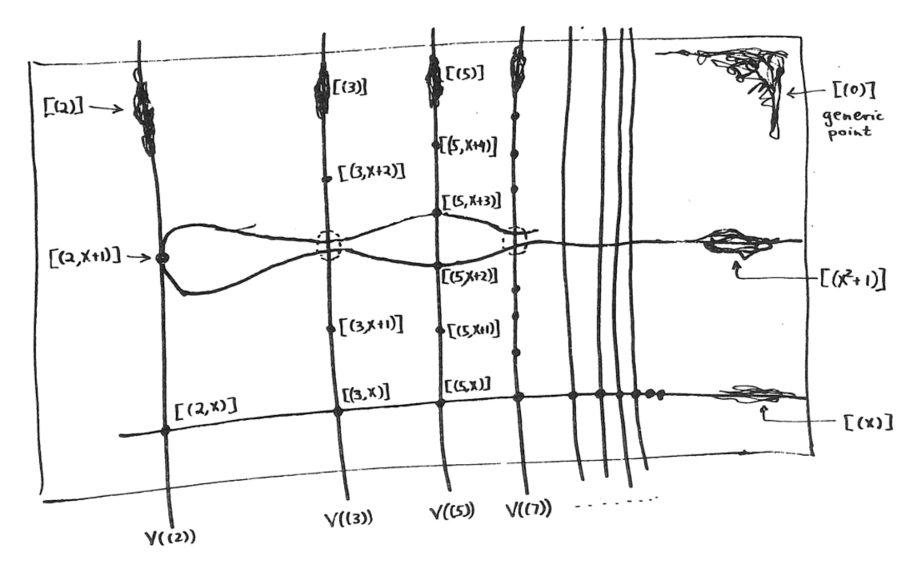
\includegraphics[width=16cm]{mumford.png}

    $\Spec \ZZ[x]$ dibujado por David Mumford
  \end{center}

  El espectro del anillo de polinomios $k[x,y]$ (donde $k$ es un cuerpo no
  necesariamente algebraicamente cerrado) tiene descripción parecida, dado que
  $\ZZ$ y $k [x]$ son dominios de ideales principales \cite[\S 1.5]{Reid-UCA}.
\end{ejemplo}

\marginpar{\footnotesize sesión 2\\13/08/19}

\begin{ejemplo}
  Sea $k$ un cuerpo algebraicamente cerrado. El teorema de los ceros implica que
  para un conjunto algebraico afín $X \subseteq \AA^n (k)$ hay biyecciones
  naturales

  \[ \begin{tikzcd}
      \Specm k [x_1,\ldots,x_n]/I(X) \ar[<->]{r} & \{ \text{puntos de }X \} \\
      \Spec k [x_1,\ldots,x_n]/I(X) \ar[<->]{r}\ar[hookrightarrow]{u} & \{ \text{subconjuntos cerrados irreducibles de }X \}\ar[hookrightarrow]{u} 
    \end{tikzcd} \]

  Bajo estas correspondencias, la topología de Zariski sobre $X$ es
  la restricción de la topología de Zariski que hemos definido arriba sobre
  $\Spec k [x_1,\ldots,x_n]/I(X)$. De hecho, todo lo que estábamos haciendo
  se ve bien parecido a las operaciones $V$ e $I$ en la geometría algebraica
  ``elemental''.

  Aunque a los puntos de $X$ corresponden solamente los ideales maximales
  (puntos cerrados del espectro), nuestra teoría tiene que trabajar con todos
  los ideales primos porque en general la preimagen de un ideal maximal no es
  necesariamente un ideal maximal. El espectro maximal, a diferencia del
  espectro primo, no es funtorial, si queremos trabajar con anillos conmutativos
  arbitrarios. Además, aunque al principio la presencia de puntos abiertos que
  no corresponden a los verdaderos puntos del conjunto $X$ parece algo
  problemático, con tiempo uno entiende que es una ventaja.
\end{ejemplo}

\begin{ejemplo}
  De nuevo, sea $k$ un cuerpo algebraicamente cerrado. Los puntos cerrados de
  $\Spec k [x,y]$ son los ideales maximales $\mathfrak{m}_{(a,b)} = (x-a,y-b)$
  que corresponden a los puntos del plano afín $(a,b) \in \AA^2 (k)$. Además,
  se tiene el punto genérico $(0)$ y un montón de otros puntos abiertos
  $\mathfrak{p}$ que corresponden a los subconjuntos cerrados irreducibles
  $Z \subsetneq \AA^2 (k)$; es decir, curvas planas irreducibles.
\end{ejemplo}

\begin{ejemplo}
  Consideremos el conjunto algebraico afín $X = V (xy) \subset \AA^2$.
  En el espectro correspondiente $\Spec k [x,y]/(xy)$ los puntos cerrados
  corresponden a los ideales maximales
  $$\mathfrak{m}_{(a,0)} = (x-a,y), ~ \mathfrak{m}_{(0,b)} = (x,y-b) \quad (a,b \in k).$$
  Además, hay dos puntos abiertos que corresponden a los ideales primos $(x)$ e
  $(y)$. Estos son los primos minimales en $k[x,y]/(xy)$. La presencia de estos
  dos puntos adicionales refleja el hecho de que $X$ tiene dos componentes
  irreducibles $V (x)$ y $V (y)$.

  \begin{center}
    \begin{tikzpicture}
      \draw (-2,0) -- (2,0);
      \draw (0,-2) -- (0,2);

      \fill[even odd rule,inner color=black,outer color=white] (-2.25,0) circle (0.2);
      \fill[even odd rule,inner color=black,outer color=white] (0,-2.25) circle (0.2);
    \end{tikzpicture}

    $\Spec k[x,y]/(xy)$
  \end{center}
\end{ejemplo}

\pagebreak
\subsection{Ejercicios}

\begin{ejerc}[\ejerccount]
  Revise la interpretación de los elementos $f\in A$ como funciones sobre
  $\Spec A$ que mencionamos en \ref{comentario:evaluacion-en-Spec}. Encuentre
  los valores de ``funciones'' $1,2,3,4,5,6 \in \ZZ$ en los puntos
  $(0), (2), (3), (5) \in \Spec\ZZ$.
\end{ejerc}

\begin{ejerc}[\ejerccount]
  \label{ejerc:espectro-de-producto}
  Demuestre que el espacio $\Spec (A\times B)$ es homeomorfo a la unión disjunta
  de $\Spec A$ y $\Spec B$. Viceversa, demuestre que si
  $\Spec C = Z_1 \cup Z_2$, donde $Z_2$ y $Z_2$ son subconjuntos cerrados
  propios y $Z_1 \cap Z_2 = \emptyset$, entonces $C \isom A\times B$ para
  $A,B \ne 0$.

  % \noindent (Indicación: véase \cite[\S 5.1, exercise 6,7]{Shafarevich-BAG-2}.)
\end{ejerc}

\begin{ejerc}[\ejerccount]
  Demuestre que $\Spec A$ es un espacio irreducible si y solo si $\Spec A[x]$ es
  irreducible.
\end{ejerc}

\begin{ejerc}[\ejerccount]
  Demuestre que $\Spec (A\otimes_\ZZ B)$ es homeomorfo
  a $\Spec A \times \Spec B$ con la topología producto.

  \noindent (Si no le sale este ejercicio, hágalo después de leer la sección
  \ref{sec:esquemas-afines} de estos apuntes.)
\end{ejerc}

\begin{ejerc}[\ejerccount]
  \label{ejerc:espectro-de-anillo-artiniano}
  Sea $A$ un anillo noetheriano. Demuestre que las siguientes condiciones son
  equivalentes.
  \begin{enumerate}
  \item[a)] $A$ es artiniano;
  \item[b)] $\Spec A$ es un espacio finito y discreto;
  \item[c)] $\Spec A$ es un espacio discreto.
  \end{enumerate}
\end{ejerc}

\begin{ejerc}[\ejerccount]
  \label{ejerc:Spec-A-Hausdorff}
  Demuestre que las siguientes condiciones son equivalentes.
  \begin{enumerate}
  \item[a)] $A$ tiene dimensión de Krull nula;
  \item[b)] todos los puntos de $\Spec A$ son cerrados;
  \item[c)] $\Spec A$ es Hausdorff.
  \end{enumerate}
\end{ejerc}

\begin{ejerc}[\ejerccount]
  \label{ejerc:Df-vacio}
  Demuestre que $D (f) = \emptyset$ si y solamente si $f\in A$ es nilpotente.
\end{ejerc}

\begin{ejerc}[\ejerccount]
  \label{ejerc:abiertos-cuasi-compactos}
  Demuestre que un subconjunto abierto $U \subseteq \Spec A$ es cuasi-compacto
  si y solamente si $U = \Spec A \setminus V (\mathfrak{a})$, donde
  $\mathfrak{a} \subseteq A$ es un ideal finitamente generado. Concluya que si
  $A$ es un anillo noetheriano, entonces cualquier subconjunto de $\Spec A$ es
  cuasi-compacto.
\end{ejerc}

\begin{ejerc}[\ejerccount]
  \label{ejerc:V-phi-m1-b}
  Sea $\phi\colon A\to B$ un homomorfismo de anillos. Demuestre que para todo
  ideal $\mathfrak{b} \subseteq B$ se tiene
  $\overline{{}^a \phi V (\mathfrak{b})} = V (\phi^{-1} (\mathfrak{b}))$.
\end{ejerc}

\begin{ejerc}[\ejerccount]
  Sea $N (A)$ el nilradical de $A$. Demuestre que el homomorfismo canónico
  ${\phi\colon A \to A/N(A)}$ induce un homeomorfismo de espacios topológicos
  ${}^a \phi\colon \Spec A/N(A) \to \Spec A$.
\end{ejerc}

\begin{ejerc}[\ejerccount]
  Sea $A \subset B$ una extensión integral de anillos. Demuestre que
  la inclusión $\phi\colon A \hookrightarrow B$ induce una aplicación
  sobreyectiva ${}^a \phi\colon \Spec B \to \Spec A$. Demuestre que ${}^a \phi$
  envía puntos cerrados a puntos cerrados.
\end{ejerc}

% % % % % % % % % % % % % % % % % % % % % % % % % % % % % %

\pagebreak
\section{Introducción a la teoría de haces}

\subsection{Prehaces y haces}

\begin{definicion}
  \label{dfn:prehaces}
  Sea $X$ un espacio topológico. Un \term{prehaz de anillos} $\mathcal{F}$ sobre
  $X$ consiste en los siguientes datos.

  \begin{enumerate}
  \item[a)] A cada subconjunto abierto $U \subseteq X$ se asigna un anillo
    $\mathcal{F} (U)$. Los elementos de $\mathcal{F} (U)$ se llaman
    las \term{secciones de $\mathcal{F}$ sobre $U$}. En particular,
    los elementos de $\mathcal{F} (X)$ se llaman las \term{secciones globales}
    de $\mathcal{F}$.

  \item[b)] A cada par de abiertos $U \subseteq V$ se asigna un homomorfismo
    de anillos
    $$\mathcal{F} (V) \to \mathcal{F} (U),$$
    llamado la \term{restricción de $V$ a $U$}. La imagen de
    $s \in \mathcal{F} (V)$ será denotada por $\left.s\right|_U$.
  \end{enumerate}

  Además, se piden los siguientes axiomas.

  \begin{enumerate}
  \item[1)] La restricción de $U$ a sí mismo es el homomorfismo identidad
    $\mathcal{F} (U) \to \mathcal{F} (U)$.

  \item[2)] Para cualesquiera tres abiertos $U \subseteq V \subseteq W$,
    la restricción de $W$ a $V$ seguida por la restricción de $V$ a $U$ coincide
    con la restricción de $W$ a $U$ de una vez:

    \[ \begin{tikzcd}
        \mathcal{F} (W) \ar{r}\ar[bend right=20]{rr} & \mathcal{F} (V) \ar{r} & \mathcal{F} (U)
      \end{tikzcd} \]
  \end{enumerate}

  Un \term{morfismo} de prehaces $\phi\colon \mathcal{F} \to \mathcal{G}$
  consiste en una familia de homomorfismos
  $\phi_U\colon \mathcal{F} (U) \to \mathcal{G} (U)$ que son compatibles con
  las restricciones en el sentido de que para todo par de abiertos
  $U \subseteq V$ el siguiente diagrama conmuta:

  \[ \begin{tikzcd}
      \mathcal{F} (V) \ar{r}{\phi_V}\ar{d} & \mathcal{G} (V)\ar{d} \\
      \mathcal{F} (U) \ar{r}{\phi_U} & \mathcal{G} (U)
    \end{tikzcd} \]
\end{definicion}

\begin{comentario}
  De la misma manera se definen los prehaces de $R$-álgebras, de grupos
  abelianos, y en general prehaces con valores en cualquier categoría.
  Sin embargo, aquí nos van a interesar solamente los prehaces de anillos.
  Solo voy a mencionar que lo más correcto sería primero estudiar los prehaces
  de conjuntos y no lo hacemos solo por falta de tiempo.
\end{comentario}

Los prehaces sobre $X$ forman una categoría que será denotada por
$\categ{PSh}_{/X}$\footnote{Del inglés \emph{presheaves}.}. Los morfismos
identidad ${\mathcal{F} \to \mathcal{F}}$ están definidos por los homomorfismos
identidad $\mathcal{F} (U) \to \mathcal{F} (U)$. Se ve que
$\phi\colon \mathcal{F} \to \mathcal{G}$ es un isomorfismo en la categoría
de prehaces si y solo si ${\phi_U\colon \mathcal{F} (U) \to \mathcal{G} (U)}$
son isomorfismos.

A partir de ahora voy a decir simplemente ``prehaz'' en lugar de ``prehaz de
anillos'', porque otros prehaces no nos servirán. También a veces no vamos
a mencionar explícitamente el espacio topológico $X$: se entiende que $X$ está
fijo y los prehaces son sobre $X$.

\begin{definicion}
  \label{dfn:haces}
  Se dice que un prehaz $\mathcal{F}$ sobre $X$ es un
  \term{haz}\footnote{\emph{Sheaf} en inglés, \emph{faisceau} en francés. Por
    alguna razón, en México se usa el término \emph{gavilla}, pero afuera de
    México mejor evitarlo. (El diccionario de la RAE: \emph{gavilla. Quizá del
      lat. *cavella, der. de cavus 'hueco entre las manos'. f. Conjunto agrupado
      de sarmientos, cañas, mieses, ramas, hierba, etc., mayor que el manojo y
      menor que el haz}.)} si para cualquier subconjunto abierto $U$ y cualquier
  recubrimiento abierto $U = \bigcup_{i\in I} U_i$ se cumplen los siguientes
  axiomas.

  \begin{enumerate}
  \item[1)] Dadas dos secciones $s,t \in \mathcal{F} (U)$, si para todo $i\in I$
    se tiene $\left.s\right|_{U_i} = \left.t\right|_{U_i}$, entonces $s = t$.

  \item[2)] Dada una familia de secciones $s_i \in \mathcal{F} (U_i)$ que
    cumplen $\left.s_i\right|_{U_i\cap U_j} = \left.s_j\right|_{U_i\cap U_j}$
    para cualesquiera $i,j\in I$, existe $s \in \mathcal{F} (U)$ tal que
    $\left.s\right|_{U_i} = s_i$ para todo $i \in I$. (Este $s$ es único gracias
    al axioma 1).)
  \end{enumerate}

  Un \term{morfismo} de haces $\phi\colon \mathcal{F} \to \mathcal{G}$ es lo
  mismo que un morfismo de prehaces. Vamos a denotar la categoría de haces sobre
  $X$ por $\categ{Sh}_{/X}$\footnote{Del inglés \emph{sheaves}.}.
\end{definicion}

\vspace{1em}

El axioma 1) significa que las secciones están definidas localmente, mientras
que 2) se llama el axioma de \term{pegamiento} porque afirma que secciones
compatibles locales pueden ser pegadas en una sección global.

\begin{comentario}
  En particular, si $U = \emptyset$, los axiomas quieren decir que
  $\mathcal{F} (\emptyset) = 0$ es el anillo nulo. (El lector que no quiere
  pensar en recubrimientos vacíos del conjunto vacío\footnote{``...mathematics
    will perish before the end of this century if the present trend for
    senseless abstraction---I call it: theory of the empty set---cannot be
    blocked up.'' ---Carl Ludwig Siegel} puede aceptarlo como una parte
  de la definición.)
\end{comentario}

\begin{comentario}
  \label{com:primer-axioma-seccion-nula}
  Puesto que estamos considerando prehaces de anillos, donde las aplicaciones
  de restricción $s \mapsto \left.s\right|_U$ son homomorfismos de anillos,
  se tiene $\left.s\right|_U = \left.t\right|_U$ si y solamente si
  $\left.(s-t)\right|_U = 0$, y el primer axioma de arriba es equivalentes
  al siguiente.
  \begin{enumerate}
  \item[$1'$)] Dada una sección $s \in \mathcal{F} (U)$, si para todo $i\in I$
    se tiene $\left.s\right|_{U_i} = 0$, entonces $s = 0$.
  \end{enumerate}
\end{comentario}

Por la definición, los haces forman una subcategoría plena de la categoría
de prehaces.

\begin{ejemplo}
  Para un espacio topológico $X$ y un abierto $U \subseteq X$, pongamos
  $$\mathcal{F} (U) \dfn \{ \text{funciones continuas } f\colon U\to \RR \}.$$
  Notamos que las funciones continuas con valores en $\RR$ forman un anillo
  (de hecho, una $\RR$-álgebra) respecto a las operaciones punto por
  punto. Tomemos como los homomorfismos de restricción
  $$\mathcal{F} (V) \to \mathcal{F} (U), \quad f \mapsto \left.f\right|_U$$
  las verdaderas restricciones de funciones. Dejo al lector verificar que todo
  esto define un haz.
\end{ejemplo}

\begin{ejemplo}
  Ahora pongamos
  $$\mathcal{F} (U) \dfn \{ \text{funciones constantes } f\colon U\to \RR \}.$$
  De la misma manera como antes, esto va a definir un prehaz. Sin embargo, este
  ya no es un haz porque no se cumple el segundo axioma: dada una familia de
  funciones constantes $f_i\colon U_i \to \RR$ compatibles en las intersecciones
  $U_i \cap U_j$, no siempre habrá una función constante $f\colon U\to \RR$ que
  se restringe a las $f_i$. ¡El problema es que las intersecciones
  $U_i \cap U_j$ pueden ser vacías! Por ejemplo, si $X = U \cup V$, donde $U$ y
  $V$ son abiertos \emph{disjuntos}, se pueden considerar dos diferentes
  funciones constantes $f\colon U\to \RR$ y $g\colon V\to \RR$.

  La condición de ser constante no es local. Sin embargo, si tomamos las
  funciones \emph{localmente constantes}\footnote{$f\colon U\to \RR$ es
    \term{localmente constante} si para todo $x\in U$ existe un entorno abierto
    $x \in U_x \subseteq U$ tal que $\left.f\right|_{U_x}$ es constante.}, estas
  sí forman un haz.
\end{ejemplo}

\begin{ejemplo}
  \label{ejemplo:prehaz-de-funciones-acotadas}
  Consideremos
  $$\mathcal{F} (U) \dfn \{ \text{funciones continuas acotadas } f\colon U\to \RR \}.$$
  De nuevo, esto dará un prehaz que no es un haz: cualquier función continua
  $f\colon U\to \RR$ no acotada siempre será localmente
  acotada\footnote{$f\colon U\to \RR$ es \term{localmente acotada} si para todo
    $x\in U$ existe un entorno abierto $x \in U_x \subseteq U$ tal que
    $\left.f\right|_{U_x}$ es acotada. El lector puede verificar que cualquier
    función continua es localmente acotada.}.
\end{ejemplo}

En el ejercicio \ref{ejerc:cociente-por-acotados} se encuentra un ejemplo de
prehaz que no cumple el primer axioma.

\subsection{Fibras}

\begin{definicion}
  \label{dfn:fibras}
  Dado un prehaz $\mathcal{F}$, su \term{fibra}\footnote{\emph{Stalk} en inglés,
    \emph{fibre} en francés.} sobre un punto $x \in X$ es el anillo
  \[ \mathcal{F}_x \dfn \dirlim_{U\ni x} \mathcal{F} (U) =
     \{ (U,s) \mid U\ni x, ~ s \in \mathcal{F} (U) \}/\sim, \]
  donde la relación de equivalencia $\sim$ viene dada por
  \[ (U,s) \sim (V,s) \iff
     \text{existe abierto } W \subseteq U\cap V
     \text{ tal que }
     x \in W \text{ y }\left.s\right|_W = \left.t\right|_W. \]
   La clase de equivalencia de $(U,s)$ se denota por $s_x$ y se llama
   el \term{germen} de $s$ en $x$.
\end{definicion}

Al principio, $\mathcal{F}_x$ es el límite directo de anillos $\mathcal{F} (U)$,
donde $U \ni x$ y los homomorfismos de transición
$\mathcal{F} (V) \to \mathcal{F} (U)$ son las restricciones. Lo que está arriba
es nada más la descripción específica del límite directo.

\begin{ejemplo}
  Dos funciones continuas $f\colon U\to \RR$ y $g\colon V\to \RR$ tienen
  el mismo germen $f_x = g_x$ en un punto $x \in U\cap V$ si $f$ y $g$ coinciden
  sobre un entorno sufientemente pequeño de $x$. Esta condición es más fuerte
  que $f (x) = g (x)$.
\end{ejemplo}

Notamos que la proyección sobre las clases de equivalencia nos da un
homomorfismo canónico
$$\mathcal{F} (U) \to \mathcal{F}_x, \quad s \mapsto s_x \dfn [(U,s)].$$

Dejo al lector verificar que un morfismo de prehaces
$\phi\colon \mathcal{F} \to \mathcal{G}$ induce homomorfismos entre las fibras
\[ \phi_x\colon \mathcal{F}_x \to \mathcal{G}_x, \quad
   [(U,s)] \mapsto [(U, \phi_U (s))]. \]
Aquí $\phi_U$ es el homomorfismo $\mathcal{F} (U) \to \mathcal{G} (U)$,
y la aplicación de arriba está bien definida, puesto que los homomorfismos
$\phi_U$ son compatibles con las restricciones (¡verifíquelo!). Gracias a esto
la fibra en $x$ es un funtor
\[ \categ{PSh}_{/X} \to \categ{CRing}, \quad
   \mathcal{F} \rightsquigarrow \mathcal{F}_x. \]
(Esta es nada más la funtorialidad de límites directos.)

\begin{lema}
  \label{lema:fibras-y-secciones-de-haz}
  Si $\mathcal{F}$ es un haz, entonces para cualquier abierto $U \subseteq X$
  el homomorfismo canónico
  \[ \mathcal{F} (U) \to \prod_{x\in U} \mathcal{F}_x, \quad
     s \mapsto (s_x)_{x \in U} \]
  es inyectivo. En palabras: las secciones de un haz están definidas por sus
  gérmenes.
\end{lema}

Para un contraejemplo cuando $\mathcal{F}$ no es un haz, haga el ejercicio
\ref{ejerc:cociente-por-acotados}.

\begin{proof}
  Si $s_x = t_x$ para todo $x \in U$, esto quiere decir que para todo $x \in U$
  existe un entorno abierto ${x \in U_x \subseteq U}$ tal que
  $\left.s\right|_{U_x} = \left.t\right|_{U_x}$. Basta entonces aplicar
  el primer axioma de haces al recubrimiento ${U = \bigcup_{x\in U} U_x}$.
\end{proof}

\begin{corolario}
  Si para dos morfismos de haces $\phi,\psi\colon \mathcal{F} \to \mathcal{G}$
  se tiene $\phi_x = \psi_x$ para todo $x\in X$, entonces $\phi = \psi$.

  \begin{proof}
    Considere el diagrama conmutativo

    \[ \begin{tikzcd}
        \mathcal{F} (U) \ar[hookrightarrow]{r}\ar[shift right=0.25em]{d}[swap]{\phi_U}\ar[shift left=0.25em]{d}{\psi_U} & \prod_{x\in U} \mathcal{F}_x\ar{d}{\prod_x \phi_x = \prod_x \psi_x} \\
        \mathcal{G} (U) \ar[hookrightarrow]{r} & \prod_{x\in U} \mathcal{G}_x
      \end{tikzcd} \]
    Aquí las flechas horizontales son inyectivas por el lema anterior.
  \end{proof}
\end{corolario}

\begin{proposicion}
  \label{prop:inyectividad-y-las-fibras}
  Para un morfismo de haces $\phi\colon \mathcal{F} \to \mathcal{G}$
  los homomorfismos $\phi_U\colon \mathcal{F} (U) \to \mathcal{G} (U)$ son
  inyectivos si y solamente si $\phi_x\colon \mathcal{F}_x \to \mathcal{G}_x$
  son inyectivos.

  \begin{proof}
    El hecho de que la inyectividad de los $\phi_U$ induce la inyectividad
    de los $\phi_x$ se deja como un ejercicio (por ejemplo, se puede usar
    la descripción de $\phi_x$ que hemos dado arriba). Ahora si
    los homomorfismos $\phi_x$ son inyectivos, podemos considerar los diagramas
    conmutativos
    \[ \begin{tikzcd}
        \mathcal{F} (U) \ar[hookrightarrow]{r}\ar{d}[swap]{\phi_U} & \prod_{x\in U} \mathcal{F}_x\ar[hookrightarrow]{d}{\prod_x \phi_x} \\
        \mathcal{G} (U) \ar{r} & \prod_{x\in U} \mathcal{G}_x
      \end{tikzcd} \]
    donde las flechas
    $\mathcal{F} (U) \hookrightarrow \prod_{x\in U} \mathcal{F}_x$ y
    $\prod_{x\in U} \mathcal{F}_x \to \prod_{x\in U} \mathcal{G}_x$ son
    inyectivas (la primera por el lema \ref{lema:fibras-y-secciones-de-haz}), y
    por lo tanto $\phi_U$ también debe ser inyectiva.
  \end{proof}
\end{proposicion}

En general, si $\phi_x\colon \mathcal{F}_x \to \mathcal{G}_x$ son sobreyectivos,
los homomorfismos $\phi_U\colon \mathcal{F} (U) \to \mathcal{G} (U)$ no tienen
por qué ser sobreyectivos (ejercicio \ref{ejerc:morfismo-exponencial}).
Este no es un defecto de la teoría; de hecho, este fenómeno está al origen
de la \term{cohomología de haces}. Sin embargo, se tiene el siguiente resultado.

\begin{proposicion}
  \label{prop:iso-sobre-las-fibras}
  Para un morfismo de haces $\phi\colon \mathcal{F} \to \mathcal{G}$
  los homomorfismos $\phi_U\colon \mathcal{F} (U) \to \mathcal{G} (U)$ son
  isomorfismos si y solamente si $\phi_x\colon \mathcal{F}_x \to \mathcal{G}_x$
  son isomorfismos. En otras palabras, $\phi$ es un isomorfismo de haces si y
  solamente si $\phi$ induce isomorfismos entre las fibras.

  \begin{proof}
    En una dirección, si $\phi$ es un isomorfismo de haces, entonces $\phi_x$
    serán isomorfismos, nada más porque todo funtor preserva isomorfismos.
    En la otra dirección, asumamos que $\phi_x$ son isomorfismos. Como ya
    probamos en \ref{prop:inyectividad-y-las-fibras}, en este caso los $\phi_U$
    serán inyectivos, y falta verificar su sobreyectividad.

    Para un abierto $U \subseteq X$, consideremos un punto $x \in U$ y
    el diagrama conmutativo

    \[ \begin{tikzcd}
        \mathcal{F} (U) \ar{r}{\phi_U}\ar{d} & \mathcal{G} (U)\ar{d} \\
        \mathcal{F}_x \ar{r}{\phi_x}[swap]{\isom} & \mathcal{G}_x
      \end{tikzcd} \]

    Para una sección $t \in \mathcal{G} (U)$ necesitamos encontrar una sección
    $s \in \mathcal{F} (U)$ tal que $\phi_U (s) = t$. Puesto que $\phi_x$
    es un isomorfismo, sabemos que $t_x$ es la imagen de alguna sección
    $s^x \in \mathcal{F} (U^x)$, donde $x \in U^x \subseteq U$. En otras
    palabras, existe un entorno suficientemente pequeño
    $x \in V^x \subseteq U^x$ tal que
    $$\left.t\right|_{V^x} = \phi_{V^x} (\left.s\right|_{V^x}).$$
    Consideremos entonces el recubrimiento abierto
    $U = \bigcup_{x\in U} V^x$. Para cualesquiera $x,y \in U$ se tiene
    \[ \phi_{V^x \cap V^y} (\left.s^x\right|_{V^x \cap V^y}) =
       \left.t\right|_{V^x\cap V^y} =
       \left.\phi\right|_{V^x\cap V^y} (\left.s^y\right|_{V^x \cap V^y}). \]
    Por la inyectividad de $\phi_{V^x \cap V^y}$, esto implica que
    $$\left.s^x\right|_{V^x \cap V^y} = \left.s^y\right|_{V^x \cap V^y}.$$
    Entonces, por el segundo axioma de haces, habrá $s \in \mathcal{F} (U)$ tal
    que $\left.s\right|_{V^x} = s^x$ para todo $x \in U$. Luego,
    $(\phi_U (s))_x = \phi_x (s_x) = t_x$ para todo $x\in U$, y por ende
    $\phi_U (s) = t$.
  \end{proof}
\end{proposicion}

\subsection{Hacificación}

Hay un modo canónico de asociar a un prehaz $\mathcal{F}$ cierto haz
$\mathcal{F}^a$. La construcción particular de $\mathcal{F}^a$ es irrelevante;
lo importante es la propiedad universal.

\begin{teorema}
  Para un prehaz $\mathcal{F}$ existe un haz $\mathcal{F}^a$, llamado
  la \term{hacificación} de $\mathcal{F}$ o el haz \term{asociado} a
  $\mathcal{F}$, junto con un morfismo de prehaces
  $\iota\colon \mathcal{F} \to \mathcal{F}^a$ que cumple la siguiente propiedad
  universal.

  Todo morfismo $\phi\colon \mathcal{F} \to \mathcal{G}$ donde $\mathcal{G}$
  es un haz se factoriza de modo único por $\iota$:

  \[ \begin{tikzcd}
      \mathcal{F} \ar{r}{\phi}\ar{d}[swap]{\iota} & \mathcal{G} \\
      \mathcal{F}^a\ar[dashed]{ur}[swap]{\exists! \widetilde{\phi}}
    \end{tikzcd} \]

  Además, $\iota_x\colon \mathcal{F}_x \to \mathcal{F}^a_x$ son isomorfismos
  para todo $x \in X$.
\end{teorema}

Por supuesto, para probar el teorema, hay que definir de alguna manera
$\mathcal{F}^a$. Intuitivamente, tenemos que modificar las secciones
$\mathcal{F} (U)$ para que se cumplan los axiomas de haces, pero sin tocar
las fibras $\mathcal{F}_x$, puesto que
$\iota_x\colon \mathcal{F}_x \xrightarrow{\isom} \mathcal{F}^a$. Prefiero omitir
la construcción de $\mathcal{F}^a_x$ porque no quiero dar la respuesta no
motivada y la motivación nos llevaría bastante lejos del tema principal de estos
apuntes. El lector interesado puede leer \cite[Chapter II]{MacLane-Moerdijk}
para la noción del \term{espacio étalé} de un prehaz. Hagamos algunas
observaciones respecto al teorema.

\begin{enumerate}
\item[1)] El típico sinsentido abstracto demuestra que la propiedad universal
  define a $\mathcal{F}^a$ de modo único salvo isomorfismo único.

\item[2)] De la propiedad universal se sigue que la hacificación es funtorial:
  un morfismo de prehaces $\phi\colon \mathcal{F} \to \mathcal{G}$ induce de
  manera canónica un morfismo entre sus hacificaciones
  $\phi\colon \mathcal{F}^a \to \mathcal{G}^a$.

  \[ \begin{tikzcd}
      \mathcal{F} \ar{r}{\phi}\ar{d}[swap]{\iota_\mathcal{F}}\ar[dashed]{dr} & \mathcal{G}\ar{d}{\iota_\mathcal{G}} \\
      \mathcal{F}^a \ar[dashed]{r}{\phi^a}[swap]{\exists!} & \mathcal{G}^a
    \end{tikzcd} \]

  Entonces, la hacificación es un funtor
  $$\categ{PSh}_{/X} \to \categ{Sh}_{/X}.$$

\item[3)] La propiedad universal significa que el funtor de hacificación es
  adjunto por la izquierda a la inclusión
  $$\categ{Sh}_{/X} \hookrightarrow \categ{PSh}_{/X}.$$
  A saber, si $\mathcal{F}$ es un prehaz y $\mathcal{G}$ es un haz, hay
  una biyección natural
  $$\Hom (\mathcal{F}^a, \mathcal{G}) \isom \Hom (\mathcal{F}, \mathcal{G}).$$
\end{enumerate}

Ahora bien, aunque no he dado ninguna construcción particular de
la hacificación, es posible calcularla usando solo la propiedad
universal. Veamos algún ejemplo.

\begin{ejemplo}
  Volvamos a \ref{ejemplo:prehaz-de-funciones-acotadas}. Sea $\mathcal{F}$
  el prehaz de funciones continuas acotadas. Este no es un haz, esencialmente
  porque la noción de ser acotado no es local. Esto nos sugiere que
  la hacificación de $\mathcal{F}$ debería ser el haz de funciones continuas
  localmente acotadas, pero cualquier función continua es localmente
  acotada. Consideremos entonces el haz de funciones continuas $\mathcal{C}$.

  Las inclusiones $\mathcal{F} (U) \subset \mathcal{C} (U)$ nos dan un morfismo
  de prehaces $\phi\colon \mathcal{F} \to \mathcal{C}$. Para una función
  continua $f\colon U\to \RR$ y un punto $x \in U$, existe un entorno abierto
  $U_x \ni x$ tal que $\left.f\right|_{U_x}$ es acotada. Esto implica
  que $\phi_x\colon \mathcal{F}_x \to \mathcal{C}_x$ son isomorfismos.

  Sea $\iota\colon \mathcal{F} \to \mathcal{F}^a$ la hacificación
  de $\mathcal{F}$. No he dicho qué es exactamente, pero conocemos su propiedad
  universal que nos da
  \[ \begin{tikzcd}
      \mathcal{F} \ar{r}{\phi}\ar{d}[swap]{\iota} & \mathcal{C} \\
      \mathcal{F}^a\ar[dashed]{ur}[swap]{\exists ! \widetilde{\phi}}
    \end{tikzcd} \]

  Ahora $\phi$ e $\iota$ inducen isomorfismos entre las fibras, así que
  $\widetilde{\phi}$ también induce isomorfismos
  $\widetilde{\phi}_x\colon \mathcal{F}^a_x \to \mathcal{C}_x$:

  \[ \begin{tikzcd}
      \mathcal{F} \ar{r}{\phi_x}[swap]{\isom}\ar{d}{\isom}[swap]{\iota_x} & \mathcal{C} \\
      \mathcal{F}^a\ar{ur}[swap]{\widetilde{\phi}_x}
    \end{tikzcd} \]

  En fin, dado que $\widetilde{\phi}$ es un morfismo de \emph{haces}, podemos
  concluir que es un isomorfismo usando el resultado
  de \ref{prop:iso-sobre-las-fibras}.
\end{ejemplo}

\begin{ejemplo}
  El mismo razonamiento demuestra que la hacificación del prehaz de funciones
  constantes es el haz de funciones localmente constantes.
\end{ejemplo}

\subsection{Imagen directa e inversa}

\marginpar{\footnotesize sesión 3\\14/08/19}

Hasta el momento nuestros haces y prehaces estaban sobre un espacio fijo $X$,
y ahora vamos a transportarlos a otros espacios mediante aplicaciones continuas.

\begin{definicion}
  \label{dfn:imagen-directa}
  Sean $f\colon X\to Y$ una aplicación continua y $\mathcal{F}$ un prehaz sobre
  $X$. Pongamos para un subconjunto abierto $V \subseteq Y$
  $$(f_* \mathcal{F}) (V) \dfn \mathcal{F} (f^{-1} (V)).$$
  Junto con las aplicaciones de restricción de $\mathcal{F}$
  (si $V \subseteq W$, entonces $f^{-1} (V) \subseteq f^{-1} (W)$), esto define
  un prehaz $f_* \mathcal{F}$ sobre $Y$, llamado la \term{imagen directa}
  de $\mathcal{F}$ respecto a $f$.
\end{definicion}

\begin{observacion}
  Si $\mathcal{F}$ es un haz, entonces $f_* \mathcal{F}$ es también un haz.

  \begin{proof}
    Ejercicio \ref{ejerc:imagen-directa-de-haz}.
  \end{proof}
\end{observacion}

Notamos que un morfismo de prehaces $\phi\colon \mathcal{F}_1 \to \mathcal{F}_2$
induce un morfismo de prehaces
$f_*\phi\colon f_*\mathcal{F}_1 \to f_*\mathcal{F}_2$:
\[ \begin{tikzcd}
    (f_*\mathcal{F}_1) (V) \ar[dashed]{r}{(f_*\phi)_V}\ar[equals]{d} & (f_*\mathcal{F}_2) (V)\ar[equals]{d} \\
    \mathcal{F}_1 (f^{-1} (V)) \ar{r}{\phi_{f^{-1} (V)}} & \mathcal{F}_2 (f^{-1} (V))
  \end{tikzcd} \]
De esta manera la imagen directa es un funtor
\[ \begin{tikzcd}
    \categ{PSh}_{/X} \ar{r}{f_*} & \categ{PSh}_{/Y}\\
    \categ{Sh}_{/X} \ar[dashed]{r}{f_*}\ar[hookrightarrow]{u} & \categ{Sh}_{/Y}\ar[hookrightarrow]{u}
  \end{tikzcd} \]

\begin{observacion}
  Sean $X \xrightarrow{f} Y \xrightarrow{g} Z$ dos aplicaciones continuas y
  $\mathcal{F}$ un prehaz sobre $X$. Luego,
  $$g_* (f_* \mathcal{F}) = (g\circ f)_* \mathcal{F}.$$

  \begin{proof}
    Por la definición,
    \[ (g_* (f_* \mathcal{F})) (W) =
       (f_* \mathcal{F}) (g^{-1} (W)) =
       \mathcal{F} (f^{-1} g^{-1} (W)) =
       \mathcal{F} ((g\circ f)^{-1} (W)). \qedhere \]
  \end{proof}
\end{observacion}

Ahora dada una aplicación continua $f\colon X\to Y$ y un prehaz $\mathcal{G}$
sobre $Y$, nos gustaría definir un prehaz sobre $X$. No se puede tomar
$U \mapsto \mathcal{G} (f (U))$ porque la imagen de un abierto no es
necesariamente abierta. Lo que se puede hacer es considerar los subconjuntos
abiertos $V \subseteq Y$ tales que $f (U) \subseteq V$ y tomar el límite directo
de las secciones $\mathcal{G} (V)$.

\begin{definicion}
  \label{dfn:imagen-inversa}
  Consideremos el prehaz
  \[ (f^+ \mathcal{G}) (U) \dfn
     \dirlim_{f (U) \subseteq V \subseteq Y} \mathcal{G} (V) =
     \{ (V,s) \mid f (U) \subseteq V \subseteq Y, ~ s \in \mathcal{G} (V) \}/\sim, \]
  donde
  \[ (V,s) \sim (V',s') \iff
     \text{existe un abierto }f (U) \subseteq W \subseteq V\cap V'
     \text{ tal que }
     \left.s'\right|_W = \left.s\right|_W. \]
  La \term{imagen inversa} de $\mathcal{G}$ es la hacificación
  $$f^{-1} \mathcal{G} \dfn (f^+ \mathcal{G})^a.$$
\end{definicion}

Si $\mathcal{G}$ es un haz, el prehaz $f^+ \mathcal{G}$ de arriba no
necesariamente será un haz, y por este motivo se toma la hacificación.
Notamos que $\mathcal{G} \rightsquigarrow f^+ \mathcal{G}$ es un funtor
(por la funtorialidad de límites directos) y la hacificación es también
un funtor. Entonces, la imagen inversa es un funtor
$$f^{-1}\colon \categ{PSh}_{/Y} \to \categ{Sh}_{/X}.$$

\begin{observacion}
  \label{obs:imagen-inversa-y-fibras}
  Sea $\mathcal{F}$ un prehaz sobre $X$. Para un punto $x \in X$ y la inclusión
  $i\colon \{ x \} \hookrightarrow X$ se tiene
  $$(i^{-1} \mathcal{F}) (\{ x \}) \isom \mathcal{F}_x.$$

  \begin{proof}
    Compare las definiciones \ref{dfn:fibras} y \ref{dfn:imagen-inversa}.
  \end{proof}
\end{observacion}

\begin{observacion}
  \label{obs:imagen-inversa-dos-aplicaciones}
  Sean $X \xrightarrow{f} Y \xrightarrow{g} Z$ dos aplicaciones continuas y
  $\mathcal{H}$ un prehaz sobre $Z$. Luego,
  $$f^{-1} (g^{-1} \mathcal{H}) \isom (g\circ f)^{-1} \mathcal{H}.$$

  \begin{proof}
    Primero,
    $$((g\circ f)^+ \mathcal{H}) (U) \dfn \dirlim_{g (f (U)) \subseteq W \subseteq Z} \mathcal{H} (W).$$
    Para un abierto $W \subseteq Z$ se tiene $g (f (U)) \subseteq W$
    si y solamente si $g (V) \subseteq W$, donde $V \subseteq Y$ es un abierto
    tal que $f (U) \subseteq V$. Esto nos permite concluir que
    $$(g\circ f)^+ \mathcal{H} = f^+ (g^+ \mathcal{H}).$$
    Tomando las hacificaciones, se obtiene el resultado deseado.
  \end{proof}
\end{observacion}

\begin{corolario}
  \label{corolario:fibras-e-imagen-inversa}
  Sean $f\colon X\to Y$ una aplicación continua y $\mathcal{G}$ un prehaz sobre
  $Y$. Entonces,
  $$(f^{-1} \mathcal{G})_x \isom \mathcal{G}_{f (x)}.$$

  \begin{proof}
    Aplique \ref{obs:imagen-inversa-y-fibras}
    y \ref{obs:imagen-inversa-dos-aplicaciones}
    a $\{ x \} \hookrightarrow X \xrightarrow{f} Y$.
  \end{proof}
\end{corolario}

Entonces, aunque nuestra construcción de la imagen inversa se ve más complicada
que la de imagen directa, es fácil entender qué sucede con las fibras bajo
la imagen inversa.

\begin{teorema}[Adjunción musical]
  \label{thm:adjuncion-musical}
  Sean $f\colon X\to Y$ una aplicación continua, $\mathcal{F}$ un haz sobre $X$
  y $\mathcal{G}$ un haz sobre $Y$. Entonces, hay una biyección natural
  \begin{align*}
    \Hom_X (f^{-1} \mathcal{G}, \mathcal{F}) & \isom \Hom_Y (\mathcal{G}, f_* \mathcal{F}),\\
    \phi & \mapsto \phi^\flat,\\
    \psi^\sharp & \mapsfrom \psi.
  \end{align*}
  En otras palabras, la imagen inversa es adjunta por la izquierda a la imagen
  directa.
\end{teorema}

Los símbolos $\flat$ y $\sharp$ vienen de la notación musical y se llaman
el \term{bemol} y \term{sostenido} respectivamente.

\begin{proof}[Bosquejo de la demostración]
  Recordemos que $f^{-1} \mathcal{G}$ es la hacificación de $f^+ \mathcal {G}$,
  y se tiene una biyección natural
  \[ \Hom_X (f^{-1} \mathcal{G}, \mathcal{F}) \isom
     \Hom_X (f^+ \mathcal{G}, \mathcal{F}). \]
  Entonces, sería suficiente encontrar una biyección
  \begin{align*}
    \Hom_X (f^+ \mathcal{G}, \mathcal{F}) & \isom \Hom_Y (\mathcal{G}, f_* \mathcal{F}),\\
    \phi & \mapsto \phi^\flat,\\
    \psi^\sharp & \mapsfrom \psi.
  \end{align*}

  Consideremos un morfismo $\phi\colon f^+ \mathcal{G} \to \mathcal{F}$. Para
  un abierto $V \subseteq Y$, se tiene $f (f^{-1} (V)) \subseteq V$, así que hay
  un homomorfismo canónico
  \[ \tag{*} \mathcal{G} (V) \to (f^+ G) (f^{-1} (V)) \dfn
     \dirlim_{f (f^{-1} (V)) \subseteq W \subseteq Y} \mathcal{G} (W) \]
  (esta es la propiedad universal de límites directos, pero en términos
  sencillos, la aplicación envía $s \in \mathcal{G} (V)$ a la clase de
  equivalencia correspondiente $(V,s)$). Podemos entonces tomar la composición
  \[ \begin{tikzcd}
      \mathcal{G} (V) \ar{r}{(*)}\ar[bend right=15]{rrr}[swap]{\rdfn \phi^\flat_V} & (f^+ G) (f^{-1} (V)) \ar{r}{\phi_{f^{-1} (V)}} & \mathcal{F} (f^{-1} (V)) \ar[equals]{r} & f_* \mathcal{F}
    \end{tikzcd} \]

  Viceversa, consideremos un morfismo
  $\psi\colon \mathcal{G} \to f_* \mathcal{F}$. Para un abierto $U \subseteq X$,
  un elemento de $(f^+ \mathcal{G}) (U)$ es una clase de equivalencia $[(V,s)]$,
  donde $f (U) \subseteq V \subseteq Y$ y $s \in \mathcal{G} (V)$. Luego,
  $U \subseteq f^{-1} (V)$, y se puede definir
  \[ \psi^\sharp_U\colon (f^+ \mathcal{G}) (U) \to \mathcal{F} (U), \quad
     [(V,s)] \mapsto \left.\psi_V (s)\right|_U. \]

  Todos los detalles se dejan al lector (hay que verificar que
  $\phi^{\flat\sharp} = \phi$, $\psi^{\sharp\flat} = \psi$, y que la biyección
  es natural en $\mathcal{F}$ y $\mathcal{G}$).
\end{proof}

Hay una construcción mucho más trasparente de la imagen inversa en términos
de los espacios étalé; el lector interesado puede consultar
\cite[Chapter II]{MacLane-Moerdijk}.

\begin{comentario}
  \label{comentario:adjuncion-musical-fibras}
  De la construcción de $\psi^\sharp$ a partir de $\psi$ que vimos la prueba
  de arriba se sigue una descripción sencilla al nivel de las fibras.
  Si $\psi\colon f^{-1} \mathcal{G} \to \mathcal{F}$, entonces los homomorfismos
  \[ \phi^\sharp_x\colon \mathcal{G}_{f (x)} = (f^{-1} \mathcal{G})_x
     \to \mathcal{F}_x \]
  vienen dados por
  $$[(V, s)] \mapsto [f^{-1} (V), \psi_V (s)],$$
  donde $f (x) \in V \subseteq Y$. Aquí hemos usado la identificación
  de \ref{corolario:fibras-e-imagen-inversa}.
\end{comentario}

\pagebreak
\subsection{Ejercicios}

\begin{ejerc}[\ejerccount]
  Sea $X = \{ x \}$ un espacio unipuntual. Demuestre que la categoría de haces
  de anillos sobre $X$ es equivalente a la categoría de anillos.
\end{ejerc}

\begin{ejerc}[\ejerccount]
  Consideremos un espacio topológico que consiste en dos puntos $X = \{ x, y \}$
  con una de las siguientes dos topologías:
  \begin{enumerate}
  \item[a)] la topología discreta;

  \item[b)] la topología donde los subconjuntos abiertos son $\emptyset$,
    $\{ x \}$, $\{ x,y \}$.
  \end{enumerate}
  En ambos casos describa todos los datos y condiciones que definen un haz sobre
  $X$. Describa las fibras en $x$ e $y$.
\end{ejerc}

\begin{ejerc}[\ejerccount]
  \label{ejerc:imagen-directa-de-haz}
  Verifique que la imagen directa de un haz es también un haz.
\end{ejerc}

\begin{ejerc}[\ejerccount]
  Demuestre la parte fácil de \ref{prop:inyectividad-y-las-fibras}:
  si los homomorfismos $\phi_U\colon \mathcal{F} (U) \to \mathcal{G} (U)$
  son inyectivos, entonces los homomorfismos entre las fibras
  $\phi_x\colon \mathcal{F}_x \to \mathcal{G}_x$ son también inyectivos.
\end{ejerc}

\begin{ejerc}[\ejerccount]
  \label{ejerc:cociente-por-acotados}
  Para un espacio topológico $X$, sea $\mathcal{C}$ el haz de funciones
  continuas (con valores en $X$) y $\mathcal{C}^b$ el haz de funciones continuas
  acotadas. Para todo abierto $U \subseteq X$ consideremos el cociente de grupos
  abelianos
  $$\mathcal{F} (U) \dfn \mathcal{C} (U)/\mathcal{C}^b (U).$$

  \begin{enumerate}
  \item[a)] Demuestre que $\mathcal{F}$ es un prehaz de grupos abelianos.
  \item[b)] Demuestre que todas las fibras $\mathcal{F}_x$ son nulas.
  \item[c)] Encuentre un espacio particular $X$ tal que $\mathcal{F}$
    no es un haz.
  \end{enumerate}
\end{ejerc}

\begin{ejerc}[\ejerccount]
  \label{ejerc:morfismo-exponencial}
  Sea $X = \CC\setminus \{ 0 \}$. Denotemos por $\O$ el haz de grupos abelianos
  \[ \O (U) \dfn \{ \text{funciones holomorfas }f\colon U\to \CC
                    \text{ respecto a la suma} \} \]
  y por $\O^\times$ el haz de grupos abelianos
  \[ \O^\times (U) \dfn
     \{ \text{funciones holomorfas sin ceros }f\colon U\to \CC
        \text{ respecto a la multiplicación} \}. \]
  Demuestre que
  $$\exp_U\colon \O (U) \mapsto \O^\times (U), \quad f \mapsto \exp (f)$$
  es un morfismo de haces que cumple
  \begin{enumerate}
  \item[a)] los homomorfismos entre las fibras
    $\exp_x\colon \O_x \to \O^\times_x$ son sobreyectivos para todo $x \in X$;
  \item[b)] el homomorfismo entre las secciones globales
    $\exp_X\colon \O (X) \to \O^\times (X)$ no es sobreyectivo.
  \end{enumerate}
\end{ejerc}

\begin{ejerc}[\ejerccount]
  Sea $\mathcal{F}$ un haz sobre $X$. Demuestre que para cualesquiera dos
  secciones $s,t \in \mathcal{F} (U)$ el conjunto
  $$\{ x\in U \mid s_x = t_x \}$$
  es abierto.
\end{ejerc}

\begin{ejerc}[\ejerccount]
  Para un espacio topológico $X$ y un anillo fijo $A$, definamos un prehaz
  tomando $\mathcal{P} (U) = A$ para todo $U \subseteq X$ y los homomorfismos
  identidad de restricción. Denotemos por $\underline{A}_X \dfn \mathcal{P}^a$
  la hacificación de este prehaz. Este se llama el \term{haz constante} con
  valores en $A$.

  Demuestre que para todo haz $\mathcal{F}$ hay una biyección natural
  \[ \Hom_{\categ{Sh}_{/X}} (\underline{A}_X, \mathcal{F}) \isom
     \Hom_\categ{CRing} (A, \mathcal{F} (X)). \]
\end{ejerc}

\begin{ejerc}[\ejerccount; haces rascacielos]
  Sea $X$ un espacio topológico. Fijemos un punto $x\in X$ y un anillo
  $A$. Pongamos para abiertos $U \subseteq X$
  \[ \mathcal{G} (U) \dfn \begin{cases}
      A, & x\in U,\\
      0, & x\notin U
    \end{cases} \]

  \begin{enumerate}
  \item[a)] Verifique que $\mathcal{G}$ junto con los homomorfismos de
    restricción evidentes es un haz sobre $X$. Este se llama el
    \term{haz rascacielos} concentrado en $x$.

  \item[b)] Calcule las fibras de $\mathcal{G}$:
    \[ \mathcal{G}_y \isom \begin{cases}
        A, & y \in \overline{\{ x \}},\\
        0, & y \notin \overline{\{ x \}}.
      \end{cases} \]

  \item[c)] Demuestre que $\mathcal{G}$ coincide con la imagen directa $i_* A$,
    donde $i\colon \{ x \} \hookrightarrow X$ es la inclusión y por abuso de
    notación $A$ denota el haz $\{ x \} \mapsto A$, $\emptyset \mapsto 0$.

  \item[d)] Demuestre que para cualquier otro haz $\mathcal{F}$ hay una
    biyección natural
    \[ \Hom_\categ{CRing} (\mathcal{F}_x, A) \isom
       \Hom_{\categ{Sh}_{/X}} (\mathcal{F}, \mathcal{G}). \]
  \end{enumerate}
\end{ejerc}

\begin{ejerc}[\ejerccount]
  Asumamos que sobre $X$ existe un haz tal que $\mathcal{F} (X) \ne 0$ y para
  cualquier abierto no vacío $U \subseteq X$ la restricción
  $\mathcal{F} (X) \to \mathcal{F} (U)$ es un isomorfismo. Demuestre que $X$
  es un espacio irreducible.
\end{ejerc}

% % % % % % % % % % % % % % % % % % % % % % % % % % % % % %

\pagebreak
\section{Espacios localmente anillados}

\subsection{Espacios anillados}

\begin{definicion}
  \label{dfn:espacios-anillados}
  Un \term{espacio anillado} $(X, \O_X)$ es un espacio topológico $X$ dotado
  de un haz de anillos $\O_X$, llamado el \term{haz estructural}. Para un punto
  $x \in X$, la fibra correspondiente de $\O_X$ se denota por $\O_{X,x}$.

  Un \term{morfismo} de espacios anillados $(X, \O_X)\to (Y, \O_Y)$ consiste en
  una aplicación continua $f\colon X\to Y$ y un morfismo de haces
  $f^\flat\colon \O_Y \to f_* \O_X$.
\end{definicion}

Notamos que gracias a la adjunción de \ref{thm:adjuncion-musical}, un morfismo
${f^\flat\colon \O_Y \to f_* \O_X}$ corresponde a un morfismo
${f^\sharp\colon f^{-1} \O_Y \to \O_X}$.

Los espacios anillados forman una categoría que será denotada por
$\categ{RS}$\footnote{Del inglés \emph{ringed spaces}.}. A saber, dados
dos morfismos
\[ (f,f^\flat)\colon (X, \O_X) \to (Y, \O_Y), \quad
   (g,g^\flat)\colon (Y, \O_Y) \to (Z, \O_Z), \]
se pueden componer las aplicaciones $f\colon X\to Y$ e $g\colon Y\to Z$, y
además, a partir de
$$f^\flat\colon \O_Y \to f_* \O_X, \quad g^\flat\colon \O_Z \to f_* \O_Y$$
se puede definir
\[ \begin{tikzcd}
\O_Z \ar{r}{g^\flat} & g_* \O_Y \ar{r}{g_* (f^\flat)} & g_* (f_* \O_X) \ar[equals]{r} & (g\circ f)_* \O_X
\end{tikzcd} \]

Normalmente el haz estructural se omite y en lugar de ``$(X,\O_X)$'' se escribe
simplemente ``$X$''\footnote{Es algo natural: por ejemplo, $X$ es un espacio
  topológico, pero la topología tampoco hace parte de la notación y normalmente
  uno no escribe cosas como ``$(X, \tau_X)$''.}. De la misma manera, en lugar
de $(f,f^\flat)$ muy a menudo se escribe simplemente ``$f$''.

\begin{definicion}
  \label{dfn:funtor-de-secciones-globales}
  A todo espacio localmente anillado $X$ se puede asociar el anillo
  correspondiente $\O_X (X)$. Además, dado un morfismo $f\colon X \to Y$,
  se puede considerar el homomorfismo de anillos correspondiente
  $$f^\flat_Y\colon \O_Y (Y) \to (f_* \O_X) (Y) = \O_X (f^{-1} (Y)) = \O_X (X).$$
  De la descripción de composición de arriba de composición de morfismos
  de espacios anillados se ve que de esta manera se obtiene un funtor
  contravariante
  \begin{align*}
    \Gamma\colon \categ{RS}^\mathrm{op} & \to \categ{CRing},\\
    X & \rightsquigarrow \O_X (X),\\
    (f\colon X \to Y) & \rightsquigarrow (f^\flat_Y\colon \O_Y (Y) \to \O_X (X)),
  \end{align*}
  llamado el \term{funtor de secciones globales}.
\end{definicion}

\subsection{Espacios localmente anillados}

A continuación nos van a interesar espacios anillados con ciertas condiciones
adicionales, llamados \term{espacios localmente anillados}.

Primero recordemos que $A$ es un \term{anillo local} si $A$ tiene un único ideal
maximal $\mathfrak{m}_A$. Esto es equivalente a tener
$A^\times = A\setminus \mathfrak{m}_A$. Se dice que un homomorfismo de anillos
locales $\phi\colon A\to B$ es \term{local} si
$\phi (\mathfrak{m}_A) \subseteq \mathfrak{m}_B$. Por ejemplo,
$\ZZ_{(p)} \hookrightarrow \QQ$ es un homomorfismo de anillos locales que
\emph{no es} local.

\begin{definicion}
  \label{dfn:espacios-localmente-anillados}
  Un \term{espacio localmente anillado} es un espacio anillado $(X,\O_X)$
  tal que todas las fibras $\O_{X,x}$ del haz estructural son anillos
  locales. En este caso el cuerpo $\kappa (x) \dfn \O_{X,x}/\mathfrak{m}_{X,x}$
  se llama el \term{cuerpo residual} en $x$.

  Un \term{morfismo} de espacios localmente anillados $(X,\O_X) \to (Y,\O_Y)$
  es un morfismo $(f,f^\flat)$ tal que los homomorfismos correspondientes
  $$f^\sharp_x\colon \O_{Y,f(x)} \to \O_{X,x}$$
  (véase \ref{comentario:adjuncion-musical-fibras}) son homomorfismos locales.
\end{definicion}

Los espacios localmente anillados forman una subcategoría (¡no plena!) de
la categoría de espacios anillados (haga el ejercicio
\ref{ejerc:composicion-de-morfismos-de-ELA}). Vamos a denotarla por
$\categ{LRS}$\footnote{Del inglés \emph{locally ringed spaces}.}.

\begin{comentario}
  Más adelante vamos a hablar de isomorfismos de espacios (localmente)
  anillados. Notamos que $(f,f^\flat)$ será un isomorfismo si y solo si
  $f\colon X\to Y$ es un homeomorfismo de espacios topológicos y
  $f^\flat\colon \O_Y \to f_* \O_X$ es un isomorfismo de haces. Lo último
  es equivalente a que $f^\sharp\colon f^{-1} \O_Y \to \O_X$ es un isomorfismo,
  o que todos los homomorfismos entre las fibras
  $f^\sharp_x\colon \O_{Y,f(x)} \to \O_{X,x}$ son isomorfismos.
\end{comentario}

\begin{ejemplo}
  \label{ejemplo:ELA-functiones-continuas}
  Sea $X$ un espacio topológico y $\mathcal{C}_X$ el haz de funciones reales
  continuas sobre $X$:
  $$\mathcal{C}_X (U) = \{ \text{funciones continuas }s\colon U\to \RR \}.$$
  Para $x \in X$ la fibra $\mathcal{C}_{X,x}$ corresponde a los gérmenes en $x$
  que son clases de equivalencia de funciones continuas $s\colon U\to \RR$,
  donde $U\ni x$, y la equivalencia viene dada por
  $$s \sim t \iff s = t \text{ en un entorno suficientemente pequeño de }x.$$
  En particular, si $s \sim t$, entonces $s (x) = t (x)$, y tiene sentido
  considerar el homomorfismo de evaluación
  $$\mathcal{C}_{X,x} \to \RR, \quad s_x \mapsto s (x).$$
  Este homomorfismo es sobreyectivo (por ejemplo, las funciones constante son
  continuas) y su núcleo es
  $$\mathfrak{m}_{X,x} = \{ s_x \mid s (x) = 0 \}.$$
  Entonces,
  $$\mathcal{C}_{X,x}/\mathfrak{m}_{X,x} \isom \RR,$$
  y el ideal $\mathfrak{m}_{X,x}$ es maximal. Ahora un germen
  $s_x \in \mathcal{C}_{X,x}\setminus \mathfrak{m}_{X,x}$ está representado por
  una función continua $s\colon U\to \RR$ tal que $s (x) \ne 0$. La continuidad
  implica que existe un entorno suficientemente pequeño $x \in V \subseteq U$
  tal que $s (v) \ne 0$ para todo $v \in V$. Luego, se puede considerar la
  función
  $$g\colon V\to \RR, \quad v \mapsto \frac{1}{f(v)},$$
  y $g_x = f_x^{-1}$. Esto demuestra que
  $\mathcal{C}_{X,x}^\times = \mathcal{C}_{X,x}\setminus \mathfrak{m}_{X,x}$,
  y por lo tanto $\mathfrak{m}_{X,x}$ es \emph{el único} ideal maximal en
  $\mathcal{C}_{X,x}$.

  Podemos concluir que $(X, \mathcal{C}_X)$ es un espacio localmente
  anillado. Ahora si $f\colon X\to Y$ es una aplicación continua, definamos
  un morfismo de haces
  $$f^\flat\colon \mathcal{C}_Y \to f_* \mathcal{C}_X$$
  mediante
  \begin{align*}
    f^\flat_V\colon \mathcal{C}_Y (V) & \to \mathcal{C}_X (f^{-1} (V)),\\
    (t\colon V\to \RR) & \mapsto (t\circ f\colon f^{-1} (V) \to \RR).
  \end{align*}

  La descripción de $f^\sharp_x$ que hemos apuntado en
  \ref{comentario:adjuncion-musical-fibras} nos da en este caso
  \[ f^\sharp_x\colon \mathcal{C}_{Y,f(x)} \to \mathcal{C}_{X,x}, \quad
     [t\colon V\to \RR] \mapsto [t\circ f\colon f^{-1} (V) \to \RR]. \]
  Se ve que $f^\sharp_x (\mathfrak{m}_{Y,f(x)}) \subseteq \mathfrak{m}_{X,x}$,
  así que $(f,f^\sharp)$ es un morfismo de espacios localmente anillados.
\end{ejemplo}

El último ejemplo explica la intuición detrás de la noción de espacio
(localmente) anillado. Uno siempre tiene que pensar en el haz estructural $\O_X$
como haz
$$\O_X (U) = \{ \text{ciertas funciones }s\colon U \to k \}.$$
(La clase de funciones debe ser definida por alguna propiedad local, para que
estas cumplan los axiomas de haces.) Ahora para un morfismo de espacios
$(f,f^\flat)\colon (X, \O_X) \to (Y, \O_Y)$ el morfismo
$f^\flat\colon \O_Y \to f_* \O_X$ intuitivamente asocia\footnote{En inglés se
  dice ``pull back functions from $Y$ to $X$'', pero no sabría traducirlo.}
a funciones $t\colon V\to k$ funciones $t\circ f\colon f^{-1} (V)\to k$.
Sin embargo, en algunas situaciones (¡y en particular en la que nos va a
interesar más adelante!), los elementos de $\O_X (U)$ no son literalmente
funciones sobre $U$, y por esto uno necesita definiciones más abstractas y
flexibles.

\vspace{1em}

En la situación más abstracta, nos gustaría interpretar las secciones
$s \in \O_X (U)$ como funciones sobre $U$ con valores en $\kappa (x)$.
Esto se hace de la siguiente manera.

\begin{definicion}
  \label{dfn:evaluacion-de-funciones}
  Sea $(X,\O_X)$ un espacio localmente anillado. Para una sección
  $s \in \O_X (U)$, donde $U \ni x$, la imagen de $s$ en el cuerpo residual en
  $x$ se denotará por $s (x)$:
  \[ \begin{tikzcd}[row sep=0pt]
      \O_X (U) \ar{r} & \O_{X,x} \ar{r} & \O_{X,x}/\mathfrak{m}_{X,x} \ar[equals]{r} & \kappa (x) \\
      s \ar[|->]{r} & s_x \ar[|->]{rr} & & \overline{s_x}
    \end{tikzcd} \]
\end{definicion}

\pagebreak

\subsection{Ejercicios}

\begin{ejerc}[\ejerccount]
  Sea $\phi\colon A\to B$ un homomorfismo de anillos locales. Demuestre que
  las siguientes condiciones son equivalentes.
  \begin{enumerate}
  \item[a)] $\phi (\mathfrak{m}_A) \subseteq \mathfrak{m}_B$;
  \item[b)] $f^{-1} (\mathfrak{m}_B) = \mathfrak{m}_A$;
  \item[c)] $A^\times = f^{-1} (B^\times)$.
  \end{enumerate}
\end{ejerc}

\begin{ejerc}[\ejerccount]
  Para $X = \RR^n$ sea $\mathcal{C}^\infty$ el haz de funciones
  diferenciables. Demuestre que $(X, \mathcal{C}^\infty)$ es un espacio
  localmente anillado. ¿Cuáles son los cuerpos residuales $\kappa (x)$?
\end{ejerc}

\begin{ejerc}[\ejerccount]
  \label{ejerc:Xf-abierto}
  Para $X = \CC$ sea $\O$ el haz de funciones holomorfas Demuestre que $(X,\O)$
  es un espacio localmente anillado. ¿Cuáles son los cuerpos residuales
  $\kappa (x)$?
\end{ejerc}

\begin{ejerc}[\ejerccount]
  Sea $(X,\O_X)$ un espacio localmente anillado. Para una sección
  $s \in \O_X (X)$ demuestre que el conjunto
  $$X_s \dfn \{ x\in X \mid s (x) \ne 0 \}$$
  es abierto. Aquí la evaluación $s (x) \in \kappa (x)$ está definida en
  \ref{dfn:evaluacion-de-funciones}.
\end{ejerc}

\begin{ejerc}[\ejerccount]
  Para la composición de dos morfismos de espacios anillados
  $$(X,\O_X) \xrightarrow{f} (Y,\O_Y) \xrightarrow{g} (Z,\O_Z)$$
  describa $(g\circ f)^\sharp$ en términos de $f^\sharp$ y $g^\sharp$.
\end{ejerc}

\begin{ejerc}[\ejerccount]
  \label{ejerc:composicion-de-morfismos-de-ELA}
  Verifique que la composición de dos morfismos de espacios localmente anillados
  es un morfismo de espacios localmente anillados.
\end{ejerc}

\begin{ejerc}[\ejerccount]
  \label{ejerc:componentes-conexas-en-ELA-1}
  Sea $(X, \O_X)$ un espacio localmente anillado.

  \begin{enumerate}
  \item[a)] Para un subconjunto abierto-cerrado $U \subseteq X$ demuestre que
    existe una sección única $e_U \in \O_X (X)$ tal que
    \begin{itemize}
    \item $\left.e_U\right|_V = 1$ para todo abierto $V \subseteq U$
    \item $\left.e_U\right|_V = 0$ para todo abierto $V \subseteq X \setminus U$.
    \end{itemize}

  \item[b)] Demuestre que esto nos da una biyección
    \[ \{ \text{subconjuntos abierto-cerrados de }X \}
       \leftrightarrow
       \{ \text{idempotentes en } \O_X (X) \}, \quad U \mapsto e_U. \]

  \item[c)] Demuestre que
    $$e_U\,e_{U'} = e_{U \cap U'}$$
    para cualesquiera abierto-cerrados $U,U' \subseteq X$.
  \end{enumerate}
\end{ejerc}

\begin{ejerc}[\ejerccount; continuación]
  \label{ejerc:componentes-conexas-en-ELA-2}
  Sea $(X, \O_X)$ un espacio localmente anillado. Demuestre que las siguientes
  condiciones son equivalentes:

  \begin{enumerate}
  \item[a)] $X$ es conexo;
  \item[b)] en $\O_X (X)$ no hay idempotentes no triviales
    (distintos de $0$ y $1$);
  \item[c)] $\O_X (X)$ no se descompone como $A\times B$ para $A,B \ne 0$.
  \end{enumerate}
\end{ejerc}

% % % % % % % % % % % % % % % % % % % % % % % % % % % % % %

\pagebreak
\section{Esquemas afines}
\label{sec:esquemas-afines}

\marginpar{\footnotesize sesión 4\\15/08/19}

\subsection{Recordatorio sobre la localización}

Vamos a necesitar varios cálculos con localizaciones, así que no estaría mal
recordar algunas definiciones y resultados.

\vspace{1em}

Dado un anillo $A$, se dice que un subconjunto $S \subset A$
es \term{multiplicativo} si $1 \in S$ y para cualesquiera $s,t \in S$ se tiene
$st \in S$. A partir de $S$ se construye la \term{localización}
$$S^{-1} A = \Bigl\{ \frac{f}{s} \Bigm| f \in A, \, s \in S \Bigr\},$$
donde la igualdad de fracciones se define mediante
$$\frac{f}{s} = \frac{g}{t} \iff u\,(ft - gs) = 0\text{ para algún }u\in S,$$
y la suma y producto de fracciones se define de la manera habitual. Se tiene
un homomorfismo
$$\iota_S\colon A\to S^{-1} A, \quad f \mapsto \frac{f}{1}$$
que cumple la siguiente propiedad universal: todo homomorfismo
$\phi\colon A\to B$ que cumple $\phi (S) \subseteq B^\times$ se factoriza
de manera única por la localización:
\[ \begin{tikzcd}
A \ar{r}{\phi}\ar{d}[swap]{\iota_S} & B \\
S^{-1} A\ar[dashed]{ur}{\exists!}[swap]{\widetilde{\phi}}
\end{tikzcd} \]
A saber, es fácil comprobar que la única opción es poner
$$\widetilde{\phi} \left(\frac{f}{s}\right) = \phi (s)\,\phi (s)^{-1}.$$

El homomorfismo canónico $\iota_S$ induce una aplicación continua
$$\iota_S^*\colon \Spec S^{-1} A \to \Spec A$$
que es un homeomorfismo sobre el subconjunto
$$\{ \mathfrak{p} \in \Spec A \mid S \cap \mathfrak{p} = \emptyset \}.$$

Nos van a interesar las siguientes situaciones particulares.

\begin{enumerate}
\item[1)] Para un elemento $f \in A$, consideremos
  $S = \{ 1,f,f^2,\ldots \}$. En este caso se obtiene
  $$A_f \dfn S^{-1} A = \Bigl\{ \frac{g}{f^n} \Bigm| g \in A, \, n = 0,1,2,\ldots \Bigr\}.$$
  El espectro correspondiente es
  $$\Spec A_f \isom \{ \mathfrak{p} \in \Spec A \mid f \notin \mathfrak{p} \} = D (f).$$

  Notamos que
  $$\frac{g}{1} = \frac{0}{1} \text{ en }A_f \iff f^n g = 0 \text{ para algún }n=0,1,2,\ldots$$

\item[2)] Para un ideal primo $\mathfrak{p} \subset A$ el conjunto
  $S = A\setminus \mathfrak{p}$ es multiplicativo y se obtiene
  \[ A_\mathfrak{p} \dfn S^{-1} A =
    \Bigl\{ \frac{f}{g} \Bigm| f,g \in A, \, g \notin \mathfrak{p} \Bigr\}. \]
  El anillo $A_\mathfrak{p}$ es local con el único ideal maximal
  $\mathfrak{p} A_\mathfrak{p}$. Se tiene
  \[ \Spec A_\mathfrak{p} \isom
     \{ \mathfrak{q} \in \Spec A \mid \mathfrak{q} \subseteq \mathfrak{p} \} =
     V (\mathfrak{p}). \]
\end{enumerate}

\subsection{Haz estructural del espectro}
\label{sec:O-Spec-A}

Nos gustaría definir un haz de anillos sobre el espectro
$X = \Spec A$. Intuitivamente, como en el ejemplo
\ref{ejemplo:ELA-functiones-continuas}, las secciones de este haz deben ser
ciertas ``funciones''. Volvamos entonces a \ref{comentario:evaluacion-en-Spec}
donde hemos definido la evaluación de $f \in A$ en $x \in \Spec A$ mediante
\[ \begin{tikzcd}[row sep=0pt]
    A \ar[->>]{r} & A/\mathfrak{p}_x \ar[hookrightarrow]{r} & \Frac (A/\mathfrak{p}_x) \\
    f \ar[|->]{r} & \overline{f} \ar[|->]{r} & f (x) \dfn \frac{\overline{f}}{1}
  \end{tikzcd} \]
De la misma manera se pueden evaluar las fracciones $\frac{g}{f^n} \in A_f$,
bajo la condición de que $f (x) \ne 0$. Entonces, los elementos de la
localización $A_f$ pueden ser interpretados como las funciones sobre el conjunto
abierto
\[ \{ x \in \Spec A \mid f (x) \ne 0 \} =
   \{ \mathfrak{p} \in \Spec A \mid f \notin \mathfrak{p} \} = D (f). \]

Esto nos sugiere poner
$$\O_X (D (f)) \dfn A_f.$$
Notamos que en particular,
$$\O_X (X) = \O_X (D(1)) = A.$$

Puesto que los conjuntos abiertos principales $D (f)$ forman una base de $X$,
sería suficiente verificar los axiomas de prehaces y haces para
$\O_X (D (f)) = A_f$, y luego $\O_X$ se extiende a $U \mapsto \O_X (U)$ para
cualquier abierto $U \subseteq X$. Para los detalles, haga el ejercicio
\ref{ejerc:B-haces-1}.

Antes de todo, necesitamos homomorfismos de restricción. Estos surgen
de la propiedad universal de de la localización.

\begin{proposicion}
  Si $D (f) \subseteq D (g)$, entonces existe un homomorfismo canónico
  $$\rho_{fg}\colon A_g \to A_f.$$
  Estos homomorfismos satisfacen
  \begin{enumerate}
  \item[1)] $\rho_{ff} = \idid\colon A_f \to A_f$,
  \item[2)] $\rho_{fg}\circ\rho_{gh} = \rho_{fh}$ para
    $D (f) \subseteq D (g) \subseteq D (h)$
    \[ \begin{tikzcd}
        A_h \ar{r}{\rho_{gh}}\ar[bend right=20]{rr}[swap]{\rho_{fh}} & A_g \ar{r}{\rho_{fg}} & A_f
      \end{tikzcd} \]
  \end{enumerate}

  \begin{proof}
    Recordemos que $D (f) \subseteq D (g)$ equivale a $f \in \sqrt{(g)}$;
    es decir, $f^n = hg$ para algún $n = 0,1,2,\ldots$ y $h \in A$. Esto implica
    que $\frac{g}{1} \in A_f^\times$. Luego, la propiedad universal de $A_g$ nos
    da el homomorfismo deseado:
    \[ \begin{tikzcd}
        A \ar{r}{\iota_f}\ar{d}[swap]{\iota_g} & A_f \\
        A_g \ar[dashed]{ur}{\exists!}[swap]{\rho_{fg}}
      \end{tikzcd} \]
    Las propiedades 1) y 2) se siguen de la unicidad de la flecha punteada.
  \end{proof}
\end{proposicion}

Notamos que en particular, si $D (f) = D (g)$, entonces las propiedades de
arriba implican que
$$\rho_{gf} = \rho_{fg}^{-1}\colon A_f \xrightarrow{\isom} A_g,$$
así que ``$\O_X (D (f)) \dfn A_f$'' está bien definido.

\begin{teorema}
  $\O_X (D (f)) \dfn A_f$ define un haz sobre $X$.

  \begin{proof}
    Como será explicado en el ejercicio \ref{ejerc:B-haces-1}, es suficiente
    verificar los axiomas de haces para los abiertos principales. Consideremos
    entonces un recubrimiento abierto
    $$D (f) = \bigcup_{i\in I} D (f_i).$$
    Puesto que $D (f)$ es cuasi-compacto (véase \ref{prof:Df-cuasi-compacto}),
    sin pérdida de generalidad, la unión es finita. Además, restringiendo $\O_X$
    a $D (f)$ (remplazando $A$ por $A_f$), se puede asumir que el recubrimiento
    tiene forma
    $$X = \bigcup_{i\in I} D (f_i).$$

    \vspace{1em}

    \textbf{El primer axioma de haces} afirma que si $s \in \O_X (X)$ cumple
    $\left.s\right|_{D (f_i)} = 0$ para todo $i$, entonces $s = 0$
    (véase comentario \ref{com:primer-axioma-seccion-nula}). Por la hipótesis,
    tenemos entonces $s \in A$ tal que $\frac{s}{1} = \frac{0}{1}$ en $A_{f_i}$
    para todo $i$, lo que significa que para todo $i$ existe
    $n_i = 0,1,2,\ldots$ tal que $f_i^{n_i} s = 0$. Notamos que
    $D (f_i) = D (f_i^{n_i})$, y gracias a esto podemos escribir
    $$X = \bigcup_{i\in I} D (f_i) = \bigcup_{i\in I} D (f_i^{n_i}).$$
    Ahora según \ref{lema:Df-en-union-de-Dfi}, existen $g_i \in A$ tales que
    $$1 = \sum_{i\in I} g_i f_i^{n_i}.$$
    Luego,
    $$s = 1\cdot s = \sum_{i\in I} g_i (f_i^{n_i} s) = 0.$$

    \vspace{1em}

    \textbf{El segundo axioma de haces} afirma que para una familia de secciones
    $s_i \in \O_X (D (f_i))$ que cumplen
    $\left.s_i\right|_{D (f_i) \cap D (f_j)} = \left.s_j\right|_{D (f_i) \cap D
      (f_j)}$ para cualesquiera $i,j\in I$, existe $s \in \O_X (X)$ tal que
    $\left.s\right|_{D (f_i)} = s_i$ para todo $i\in I$.

    Recordemos que $D (f_i) \cap D (f_j) = D (f_i f_j)$. Tenemos
    $s_i = \frac{h_i}{f_i^{n_i}} \in A_{f_i}$. El conjunto $I$ es finito,
    y se puede asumir (multiplicando el numerador por una potencia necesaria de
    $f_i$) que $s_i = \frac{h_i}{f_i^n}$, donde $n$ no depende de $i$. Ahora por
    nuestra hipótesis, para cualesquera $i,j\in I$ se cumple
    $$\frac{h_i}{f_i^n} = \frac{h_j}{f_j^n} \text{ en }A_{f_i f_j}.$$
    Lo último significa que existe algún $m_{ij}$ tal que
    $$(f_i f_j)^{m_{ij}} \, (h_i f_j^n - h_j f_i^n) = 0.$$
    De nuevo, dado que $I$ es un conjunto finito, se puede tomar $m$
    suficientemente grande independiente de $i,j$ tal que
    \[ \tag{*} f_j^{m+n} \, f_i^n h_i = f_i^{m+n} \, f_j^n h_j
       \text{ para cualesquiera }i,j\in I. \]
    Como arriba en la verificación del primer axioma, escribiendo
    $$X = \bigcup_{i\in I} D (f_i) = \bigcup_{i\in I} D (f_i^{m+n}),$$
    podemos concluir que existen $g_i \in A$ tales que
    \[ \tag{**} 1 = \sum_{j\in I} g_j f_j^{m+n}. \]

    Pongamos
    $$s \dfn \sum_{j\in I} g_j f_j^m h_j.$$

    Usando (*) y (**), calculamos
    \[ f_i^{m+n} \cdot s f_i^n =
       \sum_{j\in I} g_j (f_i^{m+n}\,f_j^m h_j)\,f_i^n =
       \sum_{j\in I} g_j (f_j^{m+n}\,f_i^m h_i)\,f_i^n =
       \left(\sum_{j\in I} g_j f_j^{m+n}\right)\,f_i^{m+n}\,h_i =
       f_i^{m+n}\,h_i. \]

    Este cálculo demuestra que
    $$\frac{s}{1} = \frac{h_i}{f_i^n} = s_i \text{ en }A_{f_i},$$
    y es lo que estábamos buscando.
  \end{proof}
\end{teorema}

En fin, podemos calcular las fibras del haz $\O_X$:
\[ \O_{X,x} = \dirlim_{x \in U} \O_X (U) =
   \dirlim_{x \in D (f)} \O_X (D (f)) =
   \dirlim_{f \notin \mathfrak{p}_x} A_f = A_{\mathfrak{p}_x}. \]
Aquí la segunda igualdad viene del hecho de que los $D (f)$ forman una base
de abiertos. Para la última igualdad, verifique que la propiedad universal
del límite directo $\dirlim_{f \notin \mathfrak{p}_x} A_f$ corresponde
a la propiedad universal de la localización $A_{\mathfrak{p}_x}$.

Todas las fibras son anillos locales, así que $(X,\O_X)$ es un espacio
localmente anillado.

\begin{ejemplo}
  Psicológicamente, es más fácil trabajar con la localización de un dominio $A$:
  en este caso existe el cuerpo de fracciones
  $$K = A_{(0)} = \Frac A = \Bigl\{ \frac{f}{g} \Bigm| f,g \in K, \, g \ne 0 \Bigr\},$$
  y para todo $f \in A$ la localización $A_f$ se identifica con un subanillo de
  $K$. Las restricciones $A_g \to A_f$ para $D (f) \subseteq D (g)$ que teníamos
  arriba son nada más las inclusiones entre subanillos.

  En un dominio, $\mathfrak{p}_\eta = (0)$ es el único ideal primo minimal
  de $A$, que corresponde al punto genérico de $X = \Spec A$. Tenemos
  $$\O_{X,\eta} = K,$$
  y por la definición del haz estructural,
  $$\O_X (D (f)) = A_f \subseteq K.$$
  Ahora dado cualquier abierto $U \subseteq \Spec X$, se tiene
  \[ \tag{*} \O_X (U) =
     \invlim_{\substack{f \in A \\ D (f) \subseteq U}} \O_X (D (f)) =
     \bigcap_{\substack{f \in A \\ D (f) \subseteq U}} A_f \]
  (haga el ejercicio \ref{ejerc:B-haces-1}), donde la intersección se considera
  en $K$. Por otra parte,
  \[ \tag{**} A_f = \bigcap_{f \notin \mathfrak{p}} A_\mathfrak{p} =
     \bigcap_{x \in D (f)} \O_{X,x}. \]
  En efecto, la inclusión ``$\subseteq$'' está clara. Para la otra inclusión,
  notamos que reemplazando $A$ por $A_f$, bastaría probar que
  $A \supseteq \bigcap_{\mathfrak{p} \in \Spec A} A_\mathfrak{p}$.
  Si $\frac{f}{g} \in K$ es un elemento tal que $\frac{f}{g} \in A_\mathfrak{p}$
  para todo $\mathfrak{p}$, entonces $g$ no está en ningún ideal maximal,
  y luego $g \in A^\times$. Podemos concluir que $\frac{f}{g} = fg^{-1} \in A$.

  Las fórmulas (*) y (**) nos dan
  \[ \O_X (U) = \bigcap_{x \in U} \O_{X,x}. \qedhere \]
\end{ejemplo}

\subsection{Funtorialidad de $(\Spec A, \O_{\Spec A})$}

Como ya sabemos, un homomorfismo de anillos $\phi\colon A\to B$ induce una
aplicación continua $f = {}^a \phi\colon X\to Y$, donde $X = \Spec B$ e
$Y = \Spec A$. Para definir un morfismo de espacios localmente anillados
$(X,\O_X) \to (Y,\O_Y)$, nos falta un morfismo de haces
$f^\flat\colon \O_Y \to f_* \O_X$. Gracias al ejercicio \ref{ejerc:B-haces-2},
bastaría definirlo para los abiertos de la forma $D (s)$; es decir, especificar
para cada $s \in A$ un homomorfismo
$$f^\flat_{D (s)}\colon \O_Y (D (s)) \to f_* \O_X (D (s)).$$
Por la definición, $\O_Y (D (s)) = A_s$ y
$f_* \O_X (D (s)) = \O_X (f^{-1} (D (s))) = \O_X (D (\phi (s))) = B_{\phi (s)}$,
así que buscamos
$$f^\flat_{D (s)}\colon A_s \to B_{\phi (s)}.$$
La única opción canónica y razonable es el homomorfismo inducido por $\phi$:
\[ \begin{tikzcd}
    A \ar{r}{\phi}\ar{d} & B\ar{d} \\
    A_s \ar[dashed]{r}{\exists!} & B_{\phi (s)}
\end{tikzcd} \]
La flecha punteada surge de la propiedad universal de $A_s$ viene dada por
$\frac{a}{s^n} \mapsto \frac{\phi (a)}{\phi (s)^n}$. No es difícil comprobar
que definidos de esta manera, los homomorfismos $f^\flat_{D (s)}$ van a conmutar
con los homomorfismos de restricción de $\O_X$ y $\O_Y$ (porque los últimos
también vienen de las propiedades universales).

Notamos que en particular, si $s = 1$, entonces se obtiene
\begin{equation}
  \label{eqn:secciones-globales-morfismo}
  f^\flat_Y = \phi\colon A \to B.
\end{equation}

Para que $(f,f^\flat)$ sea un homomorfismo de espacios \emph{localmente}
anillados, falta analizar los homomorfismos
$f^\sharp_x\colon \O_{Y,f(x)} \to \O_{X,x}$. Notamos que si $x \in \Spec B$
corresponde a un ideal primo $\mathfrak{p}_x \subset B$, entonces
$f (x) \in \Spec A$ corresponde a $\phi^{-1} (\mathfrak{p}_x)$. Uno puede
comprobar que los homomorfismos
$f^\sharp_x\colon A_{\phi^{-1} (\mathfrak{p}_x)} \to B_{\mathfrak{p}_x}$
de nuevo están inducidos por $\phi$:
\[ \begin{tikzcd}
    A \ar{r}{\phi}\ar{d} & B\ar{d} \\
    A_{\phi^{-1} (\mathfrak{p}_x)} \ar[dashed]{r}{\exists!}[swap]{f^\sharp_x} & B_{\mathfrak{p}_x}
  \end{tikzcd} \]
(la flecha punteada envía la fracción $\frac{a}{s}$, donde
$s \notin \phi^{-1} (\mathfrak{p}_x)$, a la fracción
$\frac{\phi (a)}{\phi (s)}$, donde $\phi (s) \notin \mathfrak{p}_x$).
Tenemos
$$f^\sharp_x (\phi^{-1} (\mathfrak{p}_x)) \subseteq \mathfrak{p}_x,$$
y el homomorfismo $f^\sharp_x$ sí es local.

\vspace{1em}

De esta manera hemos logrado definir un funtor contravariante
\begin{align*}
  \Spec\colon \categ{CRing}^\mathrm{op} & \to \categ{LRS},\\
  A & \rightsquigarrow (\Spec A, \O_{\Spec A}),\\
  (A\xrightarrow{\phi} B) & \rightsquigarrow \Bigl((\Spec B, \O_{\Spec B}) \xrightarrow{\Spec (\phi)} (\Spec A, \O_{\Spec A})\Bigl).
\end{align*}

Por cierto, hay muchos espacios localmente anillados. Por ejemplo,
las variedades diferenciables o complejas son casos particulares de espacios
localmente anillados. Los espectros de anillos solo forman una subcategoría muy
especial de todos los espacios localmente anillados.

\subsection{Esquemas afines}

\begin{definicion}
  \label{dfn:esquemas-afines}
  Un \term{esquema afín} es un espacio localmente anillado $(X,\O_X)$ que
  es isomorfo\footnote{En la categoría de espacios localmente anillados.}
  a $(\Spec A, \O_{\Spec A})$ para algún anillo $A$. Un \term{morfismo}
  de esquemas afines es un morfismo de espacios localmente anillados.
  Vamos a denotar la categoría de esquemas afines por $\categ{SchAf}$.
\end{definicion}

\marginpar{\footnotesize sesión 5\\
19/08/19}

\begin{ejemplo}
  \label{ejemplo:AnR}
  Para un anillo $R$, el esquema afín $\Spec R [x_1,\ldots,x_n]$ se denotará
  por $\AA^n_R$. Este es el análogo esquemático del espacio afín.
\end{ejemplo}

Resulta que la categoría de esquemas afines es simplemente antiequivalente
a la categoría de anillos conmutativos. Antes de probarlo, vamos a ver
un resultado mucho más general que se encuentra en \cite[1.6.3]{EGAI-new}.

\begin{teorema}
  \label{thm:EGA-1-6-3}
  Para cualquier espacio localmente anillado $(X,\O_X)$ y cualquier esquema afín
  $(Y,\O_Y)$ el funtor de secciones globales (definición
  \ref{dfn:funtor-de-secciones-globales}) nos da una biyección natural
  \begin{align*}
    \rho\colon \Hom_\categ{LRS} (X, Y) & \isom \Hom_\categ{CRing} (\O_Y (Y), \O_X (X)),\\
    (f\colon X \to Y) & \to (f^\flat_Y\colon \O_Y (Y) \to \O_X (X)).
  \end{align*}

  \begin{proof}
    Pongamos $\O_Y (Y) = A$ y consideremos un homomorfismo de anillos
    $\phi\colon A\to \O_X (X)$. Consideremos un punto $x \in X$.
    Para un elemento $f \in A$, consideremos el homomorfismo de
    ``evaluación en $x$''
    $$A \to \kappa (x), \quad f \mapsto \phi (f) (x),$$
    donde $\phi (f) (x)$ denota la imagen de $\phi (f) \in \O_X (X)$ en
    el cuerpo residual de $x$ (véase la definición
    \ref{dfn:evaluacion-de-funciones}). El núcleo viene dado por
    $${}^a \phi (x) \dfn \{ f \in A \mid \phi (f) (x) = 0 \}.$$
    Ahora el cociente $A / ({}^a \phi (x))$ es isomorfo a un subanillo
    de $\kappa (x)$, y entonces es un dominio. Esto significa que
    ${}^a \phi (x) \in \Spec A$. De esta manera se obtiene una aplicación
    $${}^a \phi\colon X \to \Spec A, \quad x \mapsto {}^a \phi (x).$$
    Ahora, para todo $f \in A$ se tiene
    $$({}^a \phi)^{-1} (D (f)) = X_{\phi (f)} = \{ x\in X \mid \phi (f) (x) \ne 0 \},$$
    y este conjunto es abierto en $X$ según el ejercicio
    \ref{ejerc:Xf-abierto}. Entonces, la aplicación ${}^a \phi$ es
    continua. Definamos ahora un morfismo de haces
    $${}^a \phi^\flat\colon \O_Y \to ({}^a \phi)_* \O_X.$$
    Será suficiente definirlo para las secciones sobre $D (f) \subseteq \Spec A$
    para cada $f \in A$:
    \[ {}^a \phi^\flat_{D (f)}\colon A_f \isom \O_Y (D (f)) \to
       (({}^a \phi)_* \O_X) (D (f)) =
       \O_X (({}^a \phi)^{-1} (D (f))) = \O_X (X_{\phi (f)}). \]
    Pongamos
    \begin{align*}
      \tag{*} {}^a \phi^\flat_{D (f)}\colon A_f & \to \O_X (X_{\phi (f)}),\\
      \frac{s}{f^n} & \mapsto (\left.\phi (s)\right|_{X_{\phi (f)}})\cdot (\left.\phi (f)\right|_{X_{\phi (f)}})^{-n}.
    \end{align*}
    Es fácil verificar que estas aplicaciones son compatibles con
    las restricciones $A_f \to A_g$ para $D (g) \subseteq D (f)$, así que
    se trata de un morfismo de haces. De esta manera
    $({}^a \phi, {}^a \phi^\flat)$ define un morfismo de espacios anillados.
    Por otra parte, la descripción de \ref{comentario:adjuncion-musical-fibras}
    nos dice que los homomorfismos correspondientes sobre las fibras son
    \begin{align*}
      {}^a \phi^\sharp_x\colon A_{\mathfrak{p}_y} & \to \O_{X,x},\\
      \left(\frac{s}{f^n}\right)_y & \mapsto (\phi (s)_x)\cdot (\phi (f)_x)^{-n},
    \end{align*}
    donde $y \dfn {}^a \phi (x)$. Notamos que
    $$\phi (s)_x \in \mathfrak{m}_{X,x} \iff \phi (s) (x) = 0 \iff s_y \in \mathfrak{p}_y,$$
    lo que demuestra que ${}^a \phi^\sharp_x$ es un homomorfismo local. Podemos
    concluir que se trata de un homomorfismo de espacios localmente
    anillados. Hemos definido una aplicación natural
    \begin{align*}
      \sigma\colon \Hom_\categ{CRing} (\O_Y (Y), \O_X (X)) & \isom \Hom_\categ{LRS} (X, Y),\\
      \phi & \to ({}^a \phi, {}^a \phi^\flat).
    \end{align*}

    \vspace{1em}

    Ahora vamos a verificar que la aplicación $\rho$ y $\sigma$ son aplicaciones
    mutuamente inversas. Primero, dado un homomorfismo
    $\phi\colon A \to \O_X (X)$, notamos que poniendo $f = 1$ en la fórmula (*)
    se obtiene ${}^a \phi^\flat_Y = \phi$. Esto verifica que
    $\rho\circ\sigma = \idid$.

    Viceversa, sea $(\psi,\psi^\flat)\colon X \to Y$ un morfismo de espacios
    localmente anillados. Pongamos $\phi \dfn \psi^\flat_Y$ y consideremos
    el diagrama conmutativo

    \[ \begin{tikzcd}
        \O_Y (Y) \ar{d}\ar{r}{\psi^\flat_Y \rdfn \phi} & \O_X (X) \ar{d} \\
        \O_{Y, \psi (x)} \ar[->>]{d}\ar{r}{\psi^\sharp_x} & \O_{X,x}\ar[->>]{d} \\
        \O_{Y, \psi (x)}/\mathfrak{m}_{Y,\psi (x)} \ar[equals]{d}\ar[dashed,>->]{r} & \O_{X,x}/\mathfrak{m}_{X,x}\ar[equals]{d} \\
        \kappa (\psi (x))\ar[dashed,>->]{r} & \kappa (x)
      \end{tikzcd} \]

    Aquí la flecha punteada existe gracias a la hipótesis de que $\psi^\sharp_x$
    es local, y entonces induce un monomorfismo entre los cuerpos residuales
    correspondientes. La conmutatividad del diagrama implica que dado
    $f \in A = \O_Y (Y)$, se tiene
    $$\phi (f) (x) = 0 \iff f (\psi (x)) = 0.$$
    Luego,
    \[ {}^a \phi (x) \dfn \{ f \in A \mid \phi (f) (x) = 0 \} =
       \{ f \in A \mid f (\psi (x)) = 0 \} = \psi (x). \]
    Esto demuestra que ${}^a \phi = \psi$. Por otra parte, las definiciones nos
    dicen que los diagramas
    \[ \begin{tikzcd}
        A \ar{r}{\phi}\ar{d} & \O_X (X)\ar{d} && A \ar{r}{\phi}\ar{d} & \O_X (X)\ar{d} \\
        A_{\psi (x)} \ar{r}{\psi^\sharp_x} & \O_{X,x} && A_{\psi (x)} \ar{r}{{}^a \phi^\sharp_x} & \O_{X,x}
      \end{tikzcd} \]
    son conmutativos. Sin embargo, la flecha de abajo es única por la propiedad
    universal de localización. Entonces, $\psi^\sharp_x = {}^a \phi^\sharp_x$
    para todo $x \in X$, lo que nos permite concluir que
    $\psi^\sharp = {}^a \phi^\sharp$ (véase \ref{prop:iso-sobre-las-fibras}).
  \end{proof}
\end{teorema}

\begin{corolario}
  \label{cor:antiequivalencia-esquemas-afines-anillos}
  El funtor de secciones globales $X \rightsquigarrow \O_X (X)$ nos da una
  (anti)equivalencia de categorías
  $$\categ{SchAf}^\mathrm{op} \xrightarrow{\isom} \categ{CRing}.$$

  \begin{proof}
    Dado cualquier anillo conmutativo $A$, podemos considerar el esquema afín
    correspondiente $(X,\O_X) = (\Spec A, \O_{\Spec A})$, y luego
    $\O_X (X) \isom A$, así que el funtor es esencialmente sobreyectivo.
    Por otra parte, si $X$ e $Y$ son esquemas afines, entonces el teorema
    anterior nos dice que el funtor es fielmente pleno; es decir,
    las aplicaciones correspondientes
    $$\Hom_\categ{SchAf} (X, Y) \isom \Hom_\categ{CRing} (\O_Y (Y), \O_X (X))$$
    son biyectivas.
  \end{proof}
\end{corolario}

Gracias a la última (anti)equivalencia de categorías, un esquema afín es
esencialmente lo mismo que un anillo conmutativo, solo que los morfismos
de esquemas afines van al revés. El propósito de todo el trabajo que hemos hecho
hasta el momento era interpretar anillos conmutativos como objetos geométricos.

\begin{corolario}
  Sea $Y = (Y,\O_Y)$ un espacio localmente anillado. Para que $Y$ sea un esquema
  afín, es necesario y suficiente que para cualquier otro espacio localmente
  anillado las secciones globales den una biyección
  $$\Hom_\categ{LRS} (X, Y) \isom \Hom_\categ{CRing} (\O_Y (Y), \O_X (X)).$$

  \begin{proof}
    El teorema de arriba nos dice que la condición es necesaria. Para ver que es
    suficiente, pongamos $A = \O_Y (Y)$. Notamos que las biyecciones naturales
    \[ \Hom_\categ{LRS} (X, Y) \isom
       \Hom_\categ{CRing} (A, \O_X (X)) \isom
       \Hom_\categ{LRS} (X, \Spec A) \]
    significan que hay un isomorfismo de funtores
    \[ \Hom (-, Y)\isom \Hom (-, \Spec A)\colon
       \categ{LRS}^\mathrm{op} \to \categ{Set}, \]
    así que $Y \isom \Spec A$ por el lema de Yoneda.
  \end{proof}
\end{corolario}

\begin{ejemplo}
  No estaría mal ver algún ejemplo sencillo que explique la importancia
  de trabajar con espacios \emph{localmente} anillados en lugar de todos
  los espacios anillados.

  Consideremos $X = \Spec \QQ$ e $Y = \Spec \ZZ_{(p)}$. El espacio $X$ consiste
  en un punto $\eta$, mientras que $Y$ consiste en dos puntos $y_0, y_p$ que
  corresponden a los ideales $(0), (p) \subset \ZZ_{(p)}$. El punto $y_0$
  es abierto, mientras que $y_p$ es cerrado. Consideremos la aplicación
  $$f\colon X\to Y, \quad \eta \mapsto y_p.$$
  Para definir un morfismo de espacios anillados, hay que también especificar
  un morfismo de haces
  \[ (f^\flat\colon \O_Y \to f_* \O_X) \longleftrightarrow
    (f^\sharp\colon f^{-1} \O_Y \to \O_X). \]
  Dado que $X$ es unipuntual, $f^\sharp$ es equivalente a un solo homomorfismo
  $f^\sharp_\eta\colon \O_{Y, f(\eta)} \to \O_{X,\eta}$; es decir,
  $$f^\sharp_\eta\colon \ZZ_{(p)} \to \QQ.$$
  Hay un homomorfismo único $\ZZ_{(p)} \to \QQ$, que es la inclusión
  canónica. Sin embargo, este homomorfismo no es local. De esta manera hemos
  definido un morfismo de espacios anillados $(f,f^\sharp)\colon X \to Y$, pero
  no es un morfismo de espacios localmente anillados.

  El único homomorfismo $\ZZ_{(p)} \to \QQ$ sí induce un morfismo de espacios
  localmente anillados ${(X,\O_X) \to (Y,\O_Y)}$, pero este será dado por
  $$X\to Y, \quad \eta \mapsto y_0,$$
  y no por $\eta \mapsto y_1$ como hicimos arriba.
\end{ejemplo}

\begin{ejemplo}[Subesquemas cerrados en un esquema afín]
  \label{ejemplo:subesquemas-cerrados}
  Para un esquema afín $X = \Spec A$ y un ideal $\mathfrak{a} \subset A$,
  el homomorfismo canónico $A \epi A/\mathfrak{a}$ induce un morfismo
  de esquemas afines $i\colon \Spec A/\mathfrak{a} \to \Spec A$. Este es
  un homeomorfismo sobre un subconjunto cerrado $V (\mathfrak{a}) \subseteq
  X$. Mediante la aplicación $i$, se induce una estructura de espacio localmente
  anillado sobre $V (\mathfrak{a})$. Luego, $V (\mathfrak{a}) \subset X$ se
  llama el \term{subesquema cerrado} de $X$ asociado al ideal $\mathfrak{a}$.
\end{ejemplo}

Cuidado: para subconjuntos cerrados de $\Spec A$ se tiene
$V (\mathfrak{a}^n) = V (\mathfrak{a})$, pero para subesquemas cerrados
$\Spec A/\mathfrak{a}^n$ no es lo mismo que $\Spec A/\mathfrak{a}$:
son isomorfos como espacios localmente anillados si y solo si
$A/\mathfrak{a} \isom A/\mathfrak{a}^n$.

\vspace{1em}

En la geometría algebraica clásica, uno trabaja con subconjuntos algebraicos
$X \subseteq \AA^n (k)$ (donde $k$ es un cuerpo algebraicamente cerrado)
y sus anillos de coordenadas $k [x_1,\ldots,x_n] / I (X)$, y si queremos pasar
al mundo de esquemas, hay que considerar el espectro correspondiente
$\Spec k [x_1,\ldots,x_n] / I (X)$. Sin embargo, los anillos de coordenadas
son $k$-álgebras finitamente generadas sin nilpotentes, mientras que un esquema
afín es cualquier espectro $\Spec A$, donde $A$ puede tener nilpotentes. Esto
tiene ventajas geométricas.

\begin{ejemplo}[Intersecciones esquemáticas]
  Sea $k$ un cuerpo. Consideremos el plano afín $\AA^2_k \dfn \Spec k [x,y]$.
  A los ideales $\mathfrak{a} = (y)$ y $\mathfrak{b} = (y-x^2)$ en $k [x,y]$
  corresponden los subesquemas cerrados
  \[ V (\mathfrak{a}) \isom \Spec k[x,y]/(y), \quad
     V (\mathfrak{b}) = \Spec k [x,y]/(y-x^2) \]
  que se pueden visualizar como el eje $x$ y la parábola $y = x^2$.
  La \term{intersección esquemática} de $V (\mathfrak{a})$ y $V (\mathfrak{b})$
  se define mediante
  \[ V (\mathfrak{a}) \cap V (\mathfrak{b}) \dfn
     V (\mathfrak{a} + \mathfrak{b}) \isom
     \Spec k [x,y]/(y,x^2) \isom \Spec k[x]/(x^2). \]
  Notamos que $Z \dfn \Spec k [x]/(x^2)$ es un espacio que consiste en un punto
  $z$, donde $\mathfrak{p}_z = (x^2) \subset k [x]/(x^2)$. Sin embargo, como
  un espacio localmente anillado $Z$ no es lo mismo que el punto
  $\Spec k [x]/(x) \isom \Spec k$. A saber, tenemos
  $$\O_{Z,z} \isom (k [x]/(x^2))_{(x)} \isom k \oplus k \langle x\rangle,$$
  así que
  $$\dim_k \O_{Z,z} = 2.$$
  Esto significa que $z$ es un ``punto doble'', lo que corresponde al hecho
  de que la intersección tiene multiplicidad $2$.

  \begin{center}
    \begin{tikzpicture}
      \draw[domain=-2:2,samples=100,variable=\x] plot ({\x},{\x*\x});
      \draw (2,4) node[above] {$V (y-x^2)$};
      \draw (-2,0) -- (2,0) node[right] {$V (y)$};
      \node at (0,0) [circle,fill,inner sep=1pt, label={$Z$}]{};
      \draw (-3,-0.5) -- (3,-0.5) -- (3,5) -- (-3,5) -- cycle;
      \draw (-3,5) node[below right] {$\AA^2 (k)$};
    \end{tikzpicture}
  \end{center}

  En la geometría algebraica clásica, cuando uno trabaja con intersecciones
  de curvas planas, hay que asignar una multiplicidad a cada punto
  de la intersección. En nuestro caso, ya existen puntos múltiples como objetos
  geométricos.
\end{ejemplo}

También recordemos que la teoría de intersección de curvas planas funciona bien
en el plano \emph{proyectivo} $\PP^2 (k)$ (donde $k$ es un cuerpo
algebraicamente cerrado). Más adelante vamos a definir los espacios proyectivos
como esquemas, y estos no serán afines, sino resultados de pegamiento
de esquemas afines, de la misma manera que en la geometría clásica $\PP^n (k)$
se obtiene como una unión de
$U_i \dfn \{ (x_0 : x_1 : \cdots : x_n) \mid x_i \ne 0 \} \isom \AA^n (k)$.

\pagebreak
\subsection{Ejercicios}

En los primeros dos ejercicios vamos a justificar ciertos resultados que hemos
usado varias veces en las construcciones básicas. Primero necesitamos una
definición.

\begin{definicion}
  Sean $X$ un espacio topológico y $\mathcal{B}$ una base de abiertos.

  Se dice que $\mathcal{F}$ es un \term{prehaz sobre $\mathcal{B}$} si están
  especificados
  \begin{itemize}
  \item[1)] anillos $\mathcal{F} (U)$ para $U \in \mathcal{B}$;
  \item[2)] homomorfismos de restricción
    $$\mathcal{F} (V) \to \mathcal{F} (U)\text{ para }U\subseteq V, ~ U,V\in \mathcal{B}$$
    que cumplen los axiomas habituales.
  \end{itemize}

  Un \term{morfismo de prehaces sobre $\mathcal{B}$} es una colección de
  homomorfismos
  $$\phi_U\colon \mathcal{F} (U) \to \mathcal{G} (U)\text{ para }U \in \mathcal{B}$$
  que conmutan con las restricciones.

  Se dice que $\mathcal{F}$ es un \term{haz sobre $\mathcal{B}$} si se cumplen
  los axiomas de haces para recubrimientos $U = \bigcup_{i\in I} U_i$, donde
  $U, U_i \in \mathcal{B}$.
\end{definicion}

\begin{ejerc}[\ejerccount]
  \label{ejerc:B-haces-1}
  Demuestre que todo haz sobre $\mathcal{B}$ se extiende de manera única
  a un haz sobre $X$. A saber, la extensión viene dada por
  $$\mathcal{F} (U) = \invlim_{\substack{V \subseteq U \\ V \in \mathcal{B}}} \mathcal{F} (V).$$
\end{ejerc}

\begin{ejerc}[\ejerccount]
  \label{ejerc:B-haces-2}
  Demuestre que todo morfismo de haces sobre $\mathcal{B}$ se extiende de manera
  única a un morfismo de haces sobre $X$.
\end{ejerc}

\begin{ejerc}[\ejerccount]
  Sea $X$ un esquema afín y $x \in X$ un punto cerrado que corresponde
  a un ideal maximal ${\mathfrak{m}_x \subset \O_X (X)}$. Describa la estructura
  del subesquema cerrado $V (\mathfrak{m}_x) \hookrightarrow X$.
\end{ejerc}

\begin{ejerc}[\ejerccount]
  Para los siguientes esquemas afines describa los puntos de $X$, la topología,
  los anillos $\O_X (U)$ para todos los abiertos $U \subseteq X$ y las fibras
  $\O_{X,x}$:
  \begin{enumerate}
  \item[a)] $X_1 = \Spec \CC [x]/(x^2)$;
  \item[b)] $X_2 = \Spec \CC [x]/(x^2-x)$;
  \item[c)] $X_3 = \Spec \CC [x]/(x^3 - x^2)$;
  \item[d)] $X_4 = \Spec \RR [x]/(x^2+1)$.
  \end{enumerate}
\end{ejerc}

\begin{ejerc}[\ejerccount]
  Sea $R$ un dominio de ideales principales. Para un elemento no nulo $f \in R$,
  describa el esquema afín $X = \Spec R/(f)$ (el espacio topológico subyacente,
  los anillos $\O_X (U)$ para abiertos $U \subseteq X$ y las fibras $\O_{X,x}$)
  en términos de factorización de $f$ en elementos primos (irreducibles) en $R$.
\end{ejerc}

\begin{ejerc}[\ejerccount]
  Para el esquema afín $X = \Spec \CC [x,y] / (y^2-x^3)$ y todo punto cerrado
  $p \in X$ calcule los anillos locales $\O_{X,p}$ y los ideales maximales
  correspondientes $\mathfrak{m}_{X,p} \subset \O_{X,p}$.
\end{ejerc}

\begin{ejerc}[\ejerccount; continuación]
  Sea $X$ un esquema afín. Para un punto $p \in X$ consideremos el cociente
  $\mathfrak{m}_{X,p}/\mathfrak{m}_{X,p}^2$ como un espacio vectorial sobre
  $\kappa (p)$.

  Calcule $\dim_{\kappa (p)} (\mathfrak{m}_{X,p}/\mathfrak{m}_{X,p}^2)$ para
  todos los puntos cerrados $p \in X$, donde $X = \Spec \CC [x,y] / (y^2-x^3)$.
\end{ejerc}

\begin{ejerc}[\ejerccount]
  Demuestre que si $A$ es un anillo local, entonces $\Spec A$ es conexo.

  \noindent Indicación: use los ejercicios
  \ref{ejerc:componentes-conexas-en-ELA-1} y
  \ref{ejerc:componentes-conexas-en-ELA-2}.
\end{ejerc}

\begin{ejerc}[\ejerccount]
  Demuestre que para cualesquiera $A$, $B$ hay isomorfismos canónicos
  de esquemas afines (y en particular, de espacios topológicos)
  \[ \Spec (A\times B) \isom \Spec A \sqcup \Spec B, \quad
    \Spec (A\otimes_\ZZ B) \isom \Spec A\times \Spec B. \]
\end{ejerc}

\begin{ejerc}[\ejerccount]
  Se dice que un anillo $A$ es \term{booleano} si se cumple $a^2 = a$ para todo
  $a \in A$. Los anillos booleanos forman una subcategoría plena de todos
  los anillos.

  Sean $A$ un anillo booleano y $X = \Spec A$ el esquema afín correspondiente.

  \begin{enumerate}
  \item[a)] Demuestre que todo ideal primo en $A$ es maximal y que
    $\kappa (x) = \FF_2$ para todo $x \in X$. Deduzca que se tiene una biyección
    $$\Hom (A, \FF_2) \isom \Spec A, \quad \phi \mapsto \ker(\phi).$$

  \item[b)] Demuestre que $X$ es un espacio compacto y totalmente disconexo
    y que $A \rightsquigarrow \Spec A$ nos da una equivalencia entre
    la categoría de anillos booleanos y la categoría de espacios compactos
    totalmente disconexos (donde los morfismos son aplicaciones continuas).

    A saber, el funtor cuasi-inverso a $A \rightsquigarrow \Spec A$ envía $X$
    a la $\FF_2$-álgebra de aplicaciones continuas $X \to \FF_2$ (donde $\FF_2$
    tiene la topología discreta).
  \end{enumerate}
\end{ejerc}

% % % % % % % % % % % % % % % % % % % % % % % % % % % % % %

\pagebreak
\section{Esquemas}

\marginpar{\footnotesize sesión 6\\
20/08/19}

\begin{definicion}
  \label{dfn:resticcion-de-haz}
  Sean $X$ un espacio topológico y $\mathcal{F}$ un haz sobre $X$.
  Para un subconjunto abierto $U \subseteq X$ la \term{restricción} de
  $\mathcal{F}$ a $U$ es el haz $\mathcal{F}|_U$ sobre $U$ definido mediante
  \[ \mathcal{F}|_U (V) \dfn \mathcal{F} (V) \quad
    \text{para todo abierto }V \subseteq U. \]
\end{definicion}

De hecho, $\mathcal{F}|_U$ coincide con la imagen inversa $j^{-1} \mathcal{F}$,
donde $j\colon U\hookrightarrow X$ es la inclusión.

\begin{proposicion}
  Sean $(X,\O_X)$ es un espacio (localmente) anillado y $U \subseteq X$
  un subconjunto abierto. Luego, $(U, \O_X|_U)$ es un espacio (localmente)
  anillado. Consideremos la inclusión $j\colon U \hookrightarrow X$ y definamos
  un morfismo de haces
  $$j^\flat\colon \O_X \to j_* \O_X|_U$$
  mediante las restricciones
  \[ j^\flat_V\colon \O_X (V) \to
     \O_X (V\cap U) = \O_X (j^{-1} (V)) = (j_* \O_X|_U) (V)
     \quad\text{para }V \subseteq X. \]
  Luego, $(j,j^\flat)$ es un morfismo de espacios (localmente) anillados.

  \begin{proof}
    Dejo al lector verificar los detalles necesarios.
  \end{proof}
\end{proposicion}

\subsection{Ejemplo: plano sin origen}

Es muy fácil salir del mundo de esquemas afines. Por ejemplo, un subconjunto
abierto de un esquema afín normalmente no será un esquema afín.

\begin{ejemplo}[Recta sin origen]
  Para un cuerpo algebraicamente cerrado $k$ consideremos la recta afín
  $\AA^1_k \dfn \Spec k [x]$. Sea $0 \in \AA^1_k$ el origen de la recta;
  es decir, el punto del espectro que corresponde al ideal primo
  $(x) \subset k[x]$. En este caso $U \dfn \AA^1_k \setminus \{ 0 \}$ es
  un subconjunto abierto de $\AA^1_k$ y como arriba, se obtiene un espacio
  localmente anillado $(U, \O_{\AA^1_k}|_U)$. Este es un esquema afín porque
  el subconjunto abierto $U$ coincide con la imagen de la aplicación continua
  $\Spec k [x] [x^{-1}] \hookrightarrow \Spec k [x]$ inducida por
  el homomorfismo canónico de localización $k [x] \to k [x] [x^{-1}]$.
\end{ejemplo}

\begin{ejemplo}[Plano sin origen]
  \label{ejemplo:plano-sin-origen}
  Hagamos algo parecido: tomemos el plano afín
  $X \dfn \AA^2_k \dfn \Spec k [x,y]$ y su origen $0$ que corresponde al ideal
  primo $(x,y) \subset k [x,y]$. De la misma manera,
  $U \dfn \AA^2_k \setminus \{ 0 \}$ es un subconjunto abierto de $\AA^2_k$,
  y se obtiene un espacio localmente anillado correspondiente
  $(U, \O_X|_U)$. Sin embargo, este ya no es un esquema afín. Para verlo,
  consideremos el morfismo de espacios localmente anillados
  $$(j,j^\flat)\colon (U, \O_X|_U) \hookrightarrow (\AA^2_k, \O_X)$$
  y el homomorfismo correspondiente entre las secciones globales
  $$j^\flat_X\colon \O_X (X) \to \O_X (U), \quad s \mapsto s|_U.$$
  Vamos a probar que $j^\flat_X$ es un isomorfismo de anillos. Tomemos
  el recubrimiento abierto
  $$U = D (x) \cup D (y),$$
  donde
  \[ D (x) = \{ \mathfrak{p} \in \Spec k [x,y] \mid x \notin \mathfrak{p} \},
     \quad
     D (y) = \{ \mathfrak{p} \in \Spec k [x,y] \mid y \notin \mathfrak{p} \}. \]
  Geométricamente, $D (x) = \AA^2_k \setminus V (x)$ es el plano sin el eje $y$,
  mientras que $D (y) = \AA^2_k \setminus V (y)$ es el plano sin el eje $x$.
  La unión de $D (x)$ y $D (x)$ es todo el plano salvo el origen.

  Los axiomas de haces para este recubrimiento particular nos dicen precisamente
  que hay una sucesión exacta de grupos abelianos
  \[ \begin{tikzcd}[row sep=0pt]
      0\ar{r} & \O_X (U) \ar{r} & \O_X (D (x)) \times \O_X (D (y)) \ar{r} & \O_X (D (xy)) \\
      & f \ar[|->]{r} & (f|_{D (x)}, f|_{D (y)}) \\
      & & (f,g) \ar[|->]{r} & f|_{D (xy)} - g|_{D (xy)}
    \end{tikzcd} \]
  ---el primer axioma de haces es la exactitud en $\O_X (U)$ y el segundo axioma
  es la exactitud en ${\O_X (D (x)) \times \O_X (D (y))}$. Notamos que
  \begin{align*}
    \O_X (D (x)) & \isom k [x,y] [x^{-1}],\\
    \O_X (D (y)) & \isom k [x,y] [y^{-1}],\\
    \O_X (D (x) \cap D (y)) = \O_X (D (xy)) & \isom k [x,y] [(xy)^{-1}].
  \end{align*}
  Tenemos entonces el siguiente diagrama conmutativo con filas exactas:
  \[ \begin{tikzcd}
      0\ar{r} & \O_X (U) \ar{r}\ar[dashed]{d}{\isom} & \O_X (D (x)) \times \O_X (D (y)) \ar{r}\ar{d}{\isom} & \O_X (D (xy))\ar{d}{\isom} \\
      0\ar{r} & k [x,y] \ar{r}{\Delta} & k [x,y] [x^{-1}] \times k [x,y] [y^{-1}] \ar{r} & k [x,y] [(xy)^{-1}] \\[-2em]
      & f \ar[|->]{r} & \left(\frac{f}{1},\frac{f}{1}\right) \\[-2em]
      & & \Bigl(\frac{f}{x^m},\frac{g}{y^n}\Bigr) \ar[|->]{r} & \frac{f}{x^m} - \frac{g}{y^n}
    \end{tikzcd} \]
  Aquí la exactitud de la segunda fila se comprueba fácilmente. La primera
  flecha $\Delta$ es evidentemente inyectiva, siendo inducida por
  los homomorfismos canónicos $k [x,y] \hookrightarrow k [x,y] [x^{-1}]$ y
  $k [x,y] \hookrightarrow k [x,y] [y^{-1}]$. Además, el núcleo de la segunda
  flecha coincide con la imagen de la primera:
  si $\frac{f}{x^m} = \frac{g}{y^n}$, podemos suponer que $x \nmid f$ e
  $y \nmid g$, y en este caso $y^n f = x^m g$ implica que $m = n = 0$ y $f = g$,
  usando la factorización única en $k [x,y]$.

  En el diagrama de arriba las últimas dos flechas verticales son isomorfismos,
  y por lo tanto habrá un isomorfismo inducido
  $$\O_X (U) \isom k [x,y].$$
  Todo esto nos permite concluir que $j_X^\flat$ es un isomorfismo:
  \[ \begin{tikzcd}
      \O_X (X) \ar{rr}{j^\flat_X}\ar{dr}[swap]{\isom} && \O_X (U)\ar{dl}{\isom} \\
      & k [x,y]
    \end{tikzcd} \]

  Ahora si $(U, \O_X|_U)$ fuera afín, el hecho de que las secciones globales
  $j_X^\flat$ nos dan un isomorfismo implicaría que
  $(j,j^\flat)\colon (U, \O_X|_U) \to (X, \O_X)$ es un isomorfismo, gracias
  al resultado de \ref{cor:antiequivalencia-esquemas-afines-anillos}. Pero esto
  es claramente falso: como una aplicación, $j$ no es sobreyectiva.
  Esta contradicción significa que $(U,\O_X|_U)$ no es un esquema afín.
\end{ejemplo}

El argumento de arriba se generaliza de manera obvia a una demostración de que
$\AA^n \setminus \{ 0 \}$ no es un esquema afín para cualquier $n \ge 2$.

\begin{comentario}
  El isomorfismo $j_X^\flat\colon \O_X (X) \to \O_X (U)$ es un análogo
  algebraico del \term{fenómeno de Hartogs} en el análisis complejo
  multivariable \cite[Theorem 1.2.6]{Krantz-several}. El último nos dice
  en particular que si $f\colon \CC^2 \to \CC$ es una función en dos variables
  que es holomorfa sobre $U \dfn \CC^2 \setminus \{ 0 \}$, entonces $f$
  es también holomorfa en $0$. En otras palabras, si $\O_{\CC^2}$ es
  el haz de funciones holomorfas, entonces la restricción
  $\O_{\CC^2} (\CC^2) \to \O_{\CC^2} (U)$ es un isomorfismo.

  Para las funciones en una variable, esto es falso: considere por ejemplo
  la función $f (z) = \frac{1}{z}$ que es holomorfa en todo punto salvo el
  origen $0$. De la misma manera, en el contexto algebraico, la restricción
  $i_{\AA^1_k}^\flat\colon \O_{\AA^1_k} (\AA^1_k) \to \O_{\AA^1_k} (D (x))$
  no es un isomorfismo: este es el homomorfismo canónico
  $k [x] \hookrightarrow k[x][x^{-1}]$.
\end{comentario}

Notamos que en el ejemplo \ref{ejemplo:plano-sin-origen}, aunque $U$ no es afín,
se tiene $U = D (x) \cup D (y)$, donde $D (x) \isom \Spec k [x,y] [x^{-1}]$ y
$D (y) = \Spec k [x,y] [y^{-1}]$ sí son esquemas afines. Esto nos motiva
a considerar objetos que no son necesariamente esquemas afines, pero admiten
un recubrimiento abierto por esquemas afines; es decir, \emph{localmente} se ven
como esquemas afines.

\subsection{Esquemas}

\begin{definicion}
  \label{dfn:esquemas}
  Un \term{esquema} es un espacio localmente anillado $(X, \O_X)$ que admite
  un recubrimiento abierto $X = \bigcup_{i\in I} U_i$ tal que
  $(U_i, \O_X|_{U_i})$ son esquemas afines. Tal recubrimiento se llama
  un \term{recubrimiento abierto afín}. Un \term{morfismo} de esquemas es
  un morfismo de espacios localmente anillados. La categoría de esquemas será
  denotada por $\categ{Sch}$.
\end{definicion}

Entonces, tenemos las siguientes subcategorías plenas:
$$\categ{SchAf} \subset \categ{Sch} \subset \categ{LRS}.$$

Como vimos arriba, $\AA^2_k \setminus \{ 0 \}$ es un esquema, pero no es
un esquema afín. Para construir ejemplos más interesantes de esquemas no afines,
necesitamos aprender a construir $X$ a partir de los pedazos afines $U_i$.
Lo haremos más adelante en \S\ref{sec:pegamiento}.

\begin{proposicion}
  Todo esquema $X$ tiene una base de su topología formada por
  \term{subesquemas afines abiertos}; es decir, $U \subseteq X$ tales que
  $(U, \O_X|_U)$ son afines.

  \begin{proof}
    Por la definición, $X$ puede ser cubierto por esquemas afines. Luego, cada
    esquema afín $U \isom \Spec A$ tiene como su base los conjuntos principales
    abiertos $D (f)$, donde $f \in A$. Cada $D (f)$ es afín: el homomorfismo
    canónico $A \to A_f$ induce una aplicación inyectiva
    $j\colon \Spec A_f \to \Spec A$ cuya imagen se identifica con $D (f)$,
    y los homomorfismos
    $j_x^\sharp\colon A_{\mathfrak{p}_x} \to (A_f)_{\mathfrak{p}_x}$ son
    isomorfismos para cualquier $x \in D (f)$. Entonces, $(j,j^\flat)$
    es un isomorfismo de espacios localmente anillados.
  \end{proof}
\end{proposicion}

\subsection{Esquemas relativos}
\label{sec:esquemas-relativos}

Es conveniente adoptar el punto de vista relativo y considerar las categorías
de $S$-esquemas.

\begin{definicion}
  \label{dfn:esquemas-sobre-s}
  Sea $S$ un esquema fijo. Un \term{esquema sobre $S$} es un morfismo
  de esquemas $X \to S$. Un \term{morfismo de esquemas sobre $S$} es un diagrama
  conmutativo
  \[ \begin{tikzcd}
      X\ar{rr}\ar{dr} && Y\ar{dl} \\
      & S
    \end{tikzcd} \]
  La categoría de esquemas sobre $S$ será denotada por $\categ{Sch}_{/S}$.
  Para el conjunto de morfismos $X\to Y$ sobre $S$ será conveniente escribir
  simplemente ``$\Hom_S (X,Y)$''.
\end{definicion}

\begin{comentario}
  Cuando $S = \Spec R$, en lugar de ``esquema sobre $\Spec R$'' vamos a decir
  ``esquema sobre $R$'' y en lugar de ``$\Hom_S (X,Y)$'' vamos a escribir
  ``$\Hom_R (X,Y)$''.
\end{comentario}

Por la definición, el objeto terminal en la categoría de $S$-esquemas es
$\idid\colon S\to S$.

\begin{ejemplo}
  Sea $k$ un cuerpo algebraicamente cerrado. El teorema de los ceros nos dice
  que la categoría de conjuntos algebraicos afines ${X \subseteq \AA^n (k)}$ es
  equivalente a la categoría de $k$-álgebras finitamente generadas sin
  nilpotentes $A = k[x_1,\ldots,x_n]/I$. Un morfismo de conjuntos algebraicos
  $X \to Y$ corresponde a un homomorfismo de $k$-álgebras
  (\emph{y no simplemente a un homomorfismo de anillos})
  \[ \begin{tikzcd}
      k [x_1,\ldots,x_n] / I (X) && k [x_1,\ldots,x_m] / I (Y) \ar{ll} \\
      & k \ar{ul}\ar{ur}
    \end{tikzcd} \]
  que a su vez corresponde a un morfismo de esquemas afines sobre $k$ (es decir,
  sobre $\Spec k$)
  \[ \begin{tikzcd}
      \Spec k [x_1,\ldots,x_n] / I (X)\ar{rr}\ar{dr} && \Spec k [x_1,\ldots,x_m] / I (Y)\ar{dl} \\
      & \Spec k
    \end{tikzcd} \]
  Por esto si uno quiere trabajar sobre un cuerpo $k$, en la situación
  esquemática esto corresponde a esquemas sobre $k$.
\end{ejemplo}

\begin{ejemplo}
  Supongamos que nos interesa la geometría algebraica compleja. En este contexto
  $\Spec \CC$ sería un punto. Sin embargo, los morfismos de esquemas
  $\Spec \CC \to \Spec \CC$ corresponden a homomorfismos $\CC \to \CC$;
  es decir, el grupo de automorfismos $\Aut (\CC/\QQ)$ que no es
  contable\footnote{Toda esta multitud de automorfismos no triviales se
    construye mediante el lema de Zorn. También es interesante notar que
    $\Aut (\RR/\QQ) = \{ \idid \}$: cualquier automorfismo $\RR \to \RR$ es
    automáticamente continuo y luego trivial.}. No es muy deseable tener
  un punto con muchos automorfismos, así que mejor trabajar con esquemas sobre
  $\Spec \CC$.
\end{ejemplo}

\begin{proposicion}
  \label{prop:morfismos-a-Spec-Z}
  Para todo esquema $X$ existe un morfismo único $X \to \Spec \ZZ$. En otras
  palabras, $\Spec \ZZ$ es el objeto terminal en la categoría de esquemas y todo
  esquema puede ser visto de manera única como un esquema sobre $\Spec \ZZ$.

  \begin{proof}
    El teorema \ref{thm:EGA-1-6-3}, nos da una biyección natural
    $$\Hom_\categ{Sch} (X, \Spec \ZZ) \isom \Hom_\categ{CRing} (\ZZ, \O_X (X)).$$
    Falta notar que para cualquier anillo $A$ hay un homomorfismo
    único\footnote{Por este motivo nuestros anillos tienen identidad que se
      preserva por los homomorfismos.} $\ZZ \to A$ (es decir, $\ZZ$ es el objeto
    inicial en la categoría de anillos).
  \end{proof}
\end{proposicion}

Para un resultado parecido, haga el ejercicio \ref{ejerc:morfismos-a-A1}.

\subsection{Pegamiento de haces}

\marginpar{\footnotesize sesión 7\\
21/08/19}

Los axiomas de haces nos dicen que para un recubrimiento abierto
$X = \bigcup_i U_i$, una familia de secciones compatibles
$s_i \in \mathcal{F} (U_i)$ puede ser pegada en una sección
$s \in \mathcal{F} (X)$. Ahora vamos a ver como pegar haces y sus morfismos.
La idea de pegamiento es fundamental en la geometría moderna. Para motivar
lo que sigue, empecemos por un resultado elemental.

\begin{proposicion}[Pegamiento de aplicaciones continuas]
  \label{prop:pegamiento-de-aplicaciones-continuas}
  Sean $X$ e $Y$ dos espacios topológicos y $X = \bigcup_{i\in I} U_i$
  un recubrimiento abierto. Supongamos que para cada $i\in I$ viene dada
  una aplicación continua $f_i\colon U_i \to Y$, y estas aplicaciones
  son compatibles:
  \[ f_i|_{U_i \cap U_j} = f_j|_{U_i\cap U_j}
     \quad\text{para cualesquiera }i,j \in I. \]
  Luego, existe una aplicación continua única $f\colon X\to Y$ tal que
  $f|_{U_i} = f_i$ para todo $i \in I$.

  \begin{proof}
    La condición sobre $f$ nos deja la única opción: hay que poner
    $$f (x) \dfn f_i (x)\quad\text{si }x \in U_i.$$
    Esta fórmula está bien definida gracias a la compatibilidad de
    los $f_i$. Necesitamos comprobar que la aplicación $f$ es continua.
    Para un subconjunto abierto $V \subseteq Y$ tenemos
    $$f^{-1} (V) = \bigcup_{i\in I} f_i^{-1} (V),$$
    y esta es una unión de abiertos.
  \end{proof}
\end{proposicion}

\begin{lema}[Pegamiento de morfismos de haces]
  \label{lema:pegamiento-de-morfismos-de-haces}
  Sean $X$ un espacio topológico y $\mathcal{F},\mathcal{G}$ dos haces sobre
  $X$. Asumamos que para un recubrimiento abierto $X = \bigcup_{i\in I} U_i$
  están definidos morfismos de haces sobre $U_i$
  \[ \phi_i\colon \mathcal{F}|_{U_i} \to \mathcal{G}|_{U_i}
     \quad\text{para todo }i\in I, \]
  que cumplen
  \[ \phi_i|_{U_i\cap U_j} = \phi_j|_{U_i\cap U_j}
     \quad\text{para cualesquiera }i,j\in I. \]
  Luego, existe un morfismo único $\phi\colon \mathcal{F} \to \mathcal{G}$ de
  haces sobre $X$ que cumple $\phi|_{U_i} = \phi_i$ para todo $i \in I$.

  Además, si los $\phi_i$ son isomorfismos de haces, entonces $\phi$ es también
  un isomorfismo.

  \begin{proof}
    Las condiciones nos dicen que para todo abierto $U \subseteq X$ y toda
    sección $s \in \mathcal{F} (U)$ debe cumplirse
    $$\phi_{U \cap U_i} (\left.s\right|_{U \cap U_i}) =
    \left.\phi_U (s)\right|_{U \cap U_i} =
    \phi_{i, U \cap U_i} (\left.s\right|_{U \cap U_i}).$$
    Luego, por nuestra hipótesis sobre los morfismos $\phi_i$,
    \[ \left.\phi_{i, U\cap U_i} (\left.s\right|_{U\cap U_i})\right|_{U\cap U_i\cap U_j} =
       \left.\phi_{i,U} (s)\right|_{U\cap U_i\cap U_j} =
       \left.\phi_{j,U} (s)\right|_{U\cap U_i\cap U_j} =
       \left.\phi_{j,U\cap U_j} (\left.s\right|_{U\cap U_j})\right|_{U\cap U_i\cap U_j}, \]
    y por los axiomas de haces para $\mathcal{G}$ aplicados al recubrimiento
    $U = \bigcup_i U \cap U_i$, existe una sección única $t \in \mathcal{G} (U)$
    tal que
    \[ \left.t\right|_{U\cap U_i} =
       \phi_{i,U \cap U_i} (\left.s\right|_{U\cap U_i}) =
       \left.\phi_U (s)\right|_{U\cap U_i}. \]
    Esto demuestra que $\phi$ es único y tiene que ser definido mediante
    $\phi_U (s) \dfn t$.

    \vspace{1em}

    Ahora si los $\phi_i$ son isomorfismos, consideremos sus inversos
    $\phi_i^{-1}\colon \left.\mathcal{G}\right|_{U_i} \to \left.\mathcal{F}\right|_{U_i}$.
    Tenemos
    \[ \left.\phi_i^{-1}\right|_{U_i \cap U_j} =
       (\left.\phi_i\right|_{U_i \cap U_j})^{-1} =
       (\left.\phi_j\right|_{U_i \cap U_j})^{-1} =
       \left.\phi_j^{-1}\right|_{U_i \cap U_j}, \]
    así que los $\phi_i^{-1}$ pueden ser pegados a un morfismo único
    $\phi^{-1}\colon \mathcal{G} \to \mathcal{F}$ tal que
    $\left.\phi^{-1}\right|_{U_i} = (\left.\phi\right|_{U_i})^{-1}$. Ahora
    \[ \left.(\phi^{-1} \circ \phi)\right|_{U_i} =
       \left.\id{\mathcal{F}}\right|_{U_i}, \quad
       \left.(\phi \circ \phi^{-1})\right|_{U_i} =
       \left.\id{\mathcal{G}}\right|_{U_i}, \]
    así que
    \[ \phi^{-1} \circ \phi = \id{\mathcal{F}}, \quad
       \phi \circ \phi^{-1} = \id{\mathcal{G}}, \]
    gracias a la unicidad del pegamiento.
  \end{proof}
\end{lema}

\begin{comentario}
  El lema de arriba nos dice precisamente que si $\mathcal{F}$ y $\mathcal{G}$
  son haces sobre $X$, entonces
  $$U \rightsquigarrow \Hom_{\categ{Sh}_{/U}} (\mathcal{F}|_U, \mathcal{G}|_U)$$
  define un haz (de conjuntos o de hecho de grupos abelianos) sobre $X$.
  Esta construcción tiene mucha importancia y se llama el \term{Hom interior}
  de haces.
\end{comentario}

\begin{teorema}[Pegamiento de haces]
  \label{thm:pegamiento-de-haces}
  Sean $X$ un espacio topológico y $X = \bigcup_{i\in I} U_i$ un recubrimiento
  abierto de $X$. Asumamos que se tienen los siguientes
  \term{datos de pegamiento}:
  \begin{enumerate}
  \item[a)] un haz $\mathcal{F}_i$ sobre $U_i$ para todo $i \in I$;

  \item[b)] isomorfismos
    $\phi_{ij}\colon \left.\mathcal{F}_j\right|_{U_i\cap U_j} \to \left.\mathcal{F}_i\right|_{U_i\cap U_j}$
    para cualesquiera $i,j \in I$ que satisfacen la \term{condición del cociclo}
    $$\phi_{ik} = \phi_{ij} \circ \phi_{jk} \quad\text{sobre }U_i \cap U_j \cap U_k$$
    para cualesquiera $i,j,k \in I$.
  \end{enumerate}

  Luego, existe un haz $\mathcal{F}$ sobre $X$ junto con isomorfismos
  \[ \psi_i\colon \mathcal{F}_i \xrightarrow{\isom} \left.\mathcal{F}\right|_{U_i}
     \quad\text{para todo }i \in I \]
  que cumplen
  \[ \psi_i \circ \phi_{ij} = \psi_j \quad\text{sobre }U_i \cap U_j
     \quad\text{para cualesquiera }i,j \in I. \]
  Además, $\mathcal{F}$ está definido de modo único salvo isomorfismo por estas
  condiciones.
\end{teorema}

Vamos a tratar de dar una prueba detallada, así que está ocupará un par
de páginas.

\begin{proof}
  \textbf{Primero, hagamos algunas observaciones sobre la condición del cociclo}
  \[ \begin{tikzcd}
      & \left.\mathcal{F}_j\right|_{U_i\cap U_j\cap U_k}\ar{dr}{\phi_{ij}} \\
      \left.\mathcal{F}_k\right|_{U_i\cap U_j\cap U_k} \ar{rr}{\phi_{ik}}\ar{ur}{\phi_{jk}} & & \left.\mathcal{F}_i\right|_{U_i\cap U_j\cap U_k}
    \end{tikzcd} \]
  Notamos que en particular, para $i = j = k$ se obtiene
  $\phi_{ii} = \phi_{ii} \circ \phi_{ii}$, y puesto que $\phi_{ii}$
  es un isomorfismo, esto implica que $\phi_{ii} = \idid$.
  Además, para $i = k$ se tiene
  \[ \begin{tikzcd}
      & \left.\mathcal{F}_j\right|_{U_i\cap U_j}\ar{dr}{\phi_{ij}} \\
      \left.\mathcal{F}_i\right|_{U_i\cap U_j} \ar{rr}{\phi_{ii}}[swap]{=\idid}\ar{ur}{\phi_{ji}} & & \left.\mathcal{F}_i\right|_{U_i\cap U_j}
    \end{tikzcd} \]
  así que $\phi_{ij}^{-1} = \phi_{ji}$.

  \vspace{1em}

  \textbf{Definamos $\mathcal{F}$ como un prehaz}. Pongamos para cada
  subconjunto abierto $U \subseteq X$\footnote{Tal vez psicológicamente será más
    fácil trabajar con elementos, pero en realidad lo que tenemos es cierto
    ecualizador
    $$\mathcal{F} (U) \to \prod_i \mathcal{F}_i (U \cap U_i) \rightrightarrows \prod_{i,j} \mathcal{F}_i (U \cap U_i \cap U_j)$$
    y todo lo que sigue puede ser formulado en términos de diagramas:
    los axiomas de haces también corresponden a ciertos ecualizadores,
    etcétera...}
  $$\mathcal{F} (U) \dfn \Bigl\{ (s_i)_{i \in I} \in \prod_i \mathcal{F}_i (U \cap U_i) \Bigm| \phi_{ij} (s_j|_{U\cap U_i \cap U_j}) = s_i|_{U\cap U_i \cap U_j} \text{ para cualesquiera }i,j \Bigr\}.$$
  Aquí y más adelante ``$\phi_{ij}$'' denota por abuso de notación el
  homomorfismo
  $$\phi_{ij,U\cap U_i \cap U_j}\colon \mathcal{F}_j (U\cap U_i \cap U_j) \to \mathcal{F}_j (U\cap U_i \cap U_j).$$

  \vspace{1em}

  Para $V \subseteq U$, los homomorfismos de restricción
  $\mathcal{F}_i (U \cap U_i) \to \mathcal{F}_i (V \cap U_i)$ inducen
  la restricción ${\mathcal{F} (U) \to \mathcal{F} (V)}$:

  \[ \begin{tikzcd}
      \prod_i \mathcal{F}_i (U \cap U_i) \ar{r} & \prod_i \mathcal{F}_i (V \cap U_i) \\
      \mathcal{F} (U) \ar[dashed]{r}\ar[hookrightarrow]{u} & \mathcal{F} (V)\ar[hookrightarrow]{u} \\[-2em]
      (s_i)_i \ar[|->]{r} & (s_i|_{V \cap U_i})_i
    \end{tikzcd} \]

  Hay que comprobar que si $(s_i)_i \in \mathcal{F} (V)$, entonces
  $(s_i|_{V \cap U_i})_i \in \mathcal{F} (U)$, pero esto se sigue fácilmente
  del hecho de que los $\phi_{ij}$ conmutan con las restricciones. Puesto que
  cada $\mathcal{F}_i$ es un prehaz, las restricciones para $\mathcal{F}$
  también definen un prehaz.

  % En términos de ecualizadores:
  % $$\begin{tikzcd}
  %   \mathcal{F} (U) \ar{r}\ar[dashed]{d}{\exists !} & \prod_i \mathcal{F}_i (U \cap U_i) \ar[shift left=0.25em]{r}\ar[shift right=0.25em]{r}\ar{d} & \prod_{i,j} \mathcal{F}_i (U \cap U_i \cap U_j)\ar{d} \\
  %   \mathcal{F} (V) \ar{r} & \prod_i \mathcal{F}_i (V \cap U_i) \ar[shift left=0.25em]{r} \ar[shift right=0.25em]{r} & \prod_{i,j} \mathcal{F}_i (V \cap U_i \cap U_j)
  % \end{tikzcd}$$

  \vspace{1em}

  \textbf{Verifiquemos los axiomas de haces para $\mathcal{F}$.} Sean
  $V \subseteq X$ un subconjunto abierto y $V = \bigcup_{j\in J} V_j$
  un recubrimiento abierto.

  % \[ \begin{tikzcd}
  %     & 0\ar{d} & 0\ar{d} & 0\ar{d} \\
  %     0 \ar{r} & \mathcal{F} (V) \ar{d}\ar{r} & \prod_i \mathcal{F}_i (V \cap U_i) \ar[shift left=0.25em]{r}\ar[shift right=0.25em]{r}\ar{d} & \prod_{i,i'} \mathcal{F}_i (V \cap U_i \cap U_{i'})\ar{d} \\
  %     0 \ar{r} & \prod_j \mathcal{F} (V_j) \ar[shift left=0.25em]{d}\ar[shift right=0.25em]{d}\ar{r} & \prod_{j,i} \mathcal{F}_i (V_i \cap U_i) \ar[shift left=0.25em]{r}\ar[shift right=0.25em]{r} \ar[shift left=0.25em]{d}\ar[shift right=0.25em]{d} & \prod_{j,i,i'} \mathcal{F}_i (V_j \cap U_i \cap U_{i'}) \ar[shift left=0.25em]{d}\ar[shift right=0.25em]{d} \\
  %     0 \ar{r} & \prod_{j,j'} \mathcal{F} (V_j\cap V_{j'}) \ar{r} & \prod_{j,j',i} \mathcal{F}_i (V_j\cap V_{j'} \cap U_i) \ar[shift left=0.25em]{r}\ar[shift right=0.25em]{r} & \prod_{j,j',i,i'} \mathcal{F}_i (V_j\cap V_{j'} \cap U_i \cap U_{i'})
  %   \end{tikzcd} \]

  \begin{enumerate}
  \item[1)] Asumamos que para dos secciones $s, s' \in \mathcal{F} (V)$
    se cumple $\left.s\right|_{V_j} = \left.s'\right|_{V_j}$ para todo
    $j$. Escribamos
    $$s = (s_i \in \mathcal{F}_i (V \cap U_i))_i, \quad s' = (s'_i \in \mathcal{F}_i (V \cap U_i))_i.$$
    Se tiene entonces para cualesquiera $i,j$
    $$\left.s_i\right|_{V_j \cap U_i} = \left.s'_i\right|_{V_j \cap U_i}.$$
    Ahora para todo $i$, aplicando el primer axioma de haces a $\mathcal{F}_i$
    al recubrimiento abierto ${V \cap U_i = \bigcup_{j\in J} V_j \cap U_i}$,
    podemos concluir que $s_i = s'_i$. Luego, $s = s'$.

  \item[2)] Consideremos una familia de secciones $s_j \in \mathcal{F} (V_j)$
    tales que
    $\left.s_j\right|_{V_j\cap V_{j'}} = \left.s_{j'}\right|_{V_j\cap V_{j'}}$
    para cualesquiera $j,j'$. Esto significa que se tienen
    \[ s_j = (s_{ji} \in \mathcal{F}_i (V_j \cap U_i))_i, \quad
      \phi_{ii'} (\left.s_{ji'}\right|_{V_j\cap U_i \cap U_{i'}}) =
      \left.s_{ji}\right|_{V_j\cap U_i \cap U_{i'}} \]
    que cumplen
    \[ \left.s_{ji}\right|_{V_j \cap V_{j'} \cap U_i} =
       \left.s_{j'i}\right|_{V_j \cap V_{j'} \cap U_i}. \]
    El segundo axioma de haces para $\mathcal{F}_i$ aplicado al recubrimiento
    $V \cap U_i = \bigcup_j V_j \cap U_i$ nos dice que existe una sección
    $t_i \in \mathcal{F}_i (V \cap U_i)$ que cumple
    $\left.t_i\right|_{V_j \cap U_i} = s_{ji}$. Definamos
    $$s \dfn (t_i \in \mathcal{F}_i (V \cap U_i))_i.$$
    Dejo al lector comprobar que esta sección pertenece a $\mathcal{F}
    (V)$. Luego por la construcción,
    $$\left.s\right|_{V_j} = (\left.t_i\right|_{V_j \cap U_i})_i = (s_{ji})_i = s_j.$$

    \iffalse
    Consideremos el recubrimiento abierto
    $$V\cap U_i\cap U_{i'} = \bigcup_j V_j \cap U_i \cap U_{i'}.$$
    Se tiene
    \begin{multline*}
      \left.(\left.t_i\right|_{V\cap U_i \cap U_{i'}})\right|_{V_j \cap U_i \cap U_{i'}} = \left.s_{ji}\right|_{V_j \cap U_i \cap U_{i'}} = \phi_{ii'} (\left.s_{ji'}\right|_{V_j\cap U_i \cap U_{i'}}) \\
      = \phi_{ii'} (\left.(\left.t_{i'}\right|_{V\cap U_i \cap U_{i'}})\right|_{V_j \cap U_i \cap U_{i'}}) = \left.\phi_{ii'} (\left.t_{i'}\right|_{V\cap U_i \cap U_{i'}})\right|_{V_j \cap U_i \cap U_{i'}}.
    \end{multline*}
    Ahora el primer axioma de haces para $\mathcal{F}_i$ nos permite concluir
    que
    $$\phi_{ii'} (\left.t_{i'}\right|_{V\cap U_i \cap U_{i'}}) = \left.t_i\right|_{V\cap U_i \cap U_{i'}},$$
    lo que precisamente significa que $s \in \mathcal{F} (V)$.
    \fi
  \end{enumerate}

  \vspace{1em}

  \textbf{Definamos los isomorfismos
    $\psi_i\colon \mathcal{F}_i \xrightarrow{\isom} \left.\mathcal{F}\right|_{U_i}$}.
  Notamos que hasta ahora no hemos usado ninguna hipótesis sobre los $\phi_{ij}$
  (ni que son isomorfismos, ni la condición del cociclo), pero es lo que
  necesitamos para definir los $\psi_i$. Recordemos que estos tienen que cumplir
  \[ \begin{tikzcd}
      & \left.\mathcal{F}_i\right|_{U_i\cap U_j}\ar{dr}{\psi_i} \\
      \left.\mathcal{F}_j\right|_{U_i \cap U_j} \ar{rr}{\psi_j}\ar{ur}{\phi_{ij}} && \left.\mathcal{F}\right|_{U_i \cap U_j}
    \end{tikzcd} \]

  Hay un morfismo de haces evidente
  $\pi_i\colon \left.\mathcal{F}\right|_{U_i} \to \mathcal{F}_i$ dado por
  \begin{align*}
    \pi_{i,U}\colon \mathcal{F} (U) & \to \mathcal{F}_i (U),\\
    s \dfn (s_j \in \mathcal{F}_j (U \cap U_j))_j & \mapsto s_i
  \end{align*}
  para un subconjunto abierto $U \subseteq U_i$. Definamos su inverso
  $\psi_i\colon \mathcal{F}_i \to \left.\mathcal{F}\right|_{U_i}$ mediante
  \begin{align*}
    \psi_i\colon \mathcal{F}_i (U) & \to \mathcal{F} (U),\\
    s_i & \mapsto s \dfn (\phi_{ji} (\left.s_i\right|_{U_i \cap U_j}) \in \mathcal{F}_j (U \cap U_j))_j.
  \end{align*}
  Hay que ver que $s \in \mathcal{F} (U)$:
  \[ \phi_{jj'} (\left.t_{j'}\right|_{U_i\cap U_j \cap U_{j'}}) =
     \left.t_j\right|_{U_i\cap U_j \cap U_{j'}},
     \quad\text{donde }t_j \dfn \phi_{ji} (\left.s_i\right|_{U_i \cap U_j}). \]
  Pero esta es precisamente la condición del cociclo
  $\phi_{jj'} \circ \phi_{j'i} = \phi_{ji}$ sobre $U_i \cap U_j \cap
  U_{j'}$. Las condiciones que hemos impuesto sobre los elementos de
  $\mathcal{F} (U)$ aseguran que $\pi_i$ y $\psi_i$ son mutualmente inversos. La
  identidad $\psi_i \circ \phi_{ij} = \psi_j$ viene de la condición del cociclo:
  \[ \psi_i \circ \phi_{ij} (s_j) =
     (\phi_{ki} \circ \phi_{ij} (s_j))_k =
     (\phi_{kj} (s_j))_k = \psi_j (s_j). \]

  \vspace{1em}

  \textbf{En fin, comprobemos que $\mathcal{F}$ es único salvo
    isomorfismo}. Supongamos que hay dos haces $\mathcal{F}$ y $\mathcal{F}'$
  que cumplen las condiciones del teorema. En este caso tenemos isomorfismos
  $$\psi'_i\circ \psi_i^{-1}\colon \left.\mathcal{F}\right|_{U_i}
  \xrightarrow{\isom} \mathcal{F}_i
  \xrightarrow{\isom} \left.\mathcal{F}'\right|_{U_i}$$
  que cumplen
  $$\left.(\psi'_i\circ \psi_i^{-1})\right|_{U_i \cap U_j} =
  \left.(\psi'_i\circ \phi_{ij} \circ \phi_{ij}^{-1} \circ \psi_i^{-1})\right|_{U_i \cap U_j} =
  \left.(\psi'_i\circ \phi_{ij} \circ (\psi_i \circ \phi_{ij})^{-1})\right|_{U_i \cap U_j} =
  \left.(\psi'_j \circ \psi_j^{-1})\right|_{U_i \cap U_j}.$$
  Entonces, por el lema \ref{lema:pegamiento-de-morfismos-de-haces},
  los isomorfismos $\psi'_i\circ \psi_i^{-1}$ se pegan a un isomorfismo único
  $\mathcal{F} \xrightarrow{\isom} \mathcal{F}'$.
\end{proof}

\subsection{Pegamiento de esquemas}
\label{sec:pegamiento}

Ahora vamos a pegar espacios localmente anillados, y en particular
esquemas. Como antes, es más fácil pegar morfismos.

\begin{proposicion}
  Sean $(X, \O_X)$ e $(Y, \O_Y)$ dos espacios localmente anillados
  y $X = \bigcup_{i\in I} U_i$ un recubrimiento abierto. Supongamos que para
  cada $i$ están definidos morfismos de espacios localmente anillados
  $$f_i\colon (U_i, \O_X|_{U_i}) \to (Y, \O_Y)$$
  tales que $f_i|_{U_i\cap U_j} = f_j|_{U_i\cap U_j}$ para cualesquiera
  $i,j \in I$. Luego, existe un morfismo único $f\colon (X, \O_X)\to (Y, \O_Y)$
  tal que $f|_{U_i} = f_i$ para todo $i\in I$.

  \begin{proof}
    Primero, las aplicaciones continuas $f_i$ se pegan en $f\colon X\to Y$,
    como vimos en \ref{prop:pegamiento-de-aplicaciones-continuas}.
    Además, se tienen morfismos compatibles
    $f_i^\sharp\colon f_i^{-1} \O_Y \to \O_X|_{U_i}$, y el lema
    \ref{lema:pegamiento-de-morfismos-de-haces} nos permite pegarlos
    en $f^\sharp\colon f^{-1} \O_Y \to \O_X$. En fin, si $x \in U_i$, entonces
    $f^\sharp_x = f^\sharp_{i,x}$, así que cada $f^\sharp_x$ es un homomorfismo
    local.
  \end{proof}
\end{proposicion}

\marginpar{\footnotesize sesión 8 \\
22/08/19}

\begin{teorema}[Pegamiento de espacios localmente anillados]
  \label{thm:pegamiento-de-ELA}
  Supongamos que están especificados los siguientes \term{datos de pegamiento}.

  \begin{enumerate}
  \item[1)] Una familia de espacios localmente anillados $(X_i, \O_{X_i})$
    indexados por $i \in I$.

  \item[2)] Subconjuntos abiertos $U_{ij} \subseteq X_i$ para cualesquiera
    $i,j \in I$.

  \item[3)] isomorfismos de espacios localmente anillados
    \[ \phi_{ij}\colon (U_{ij}, \O_{X_i}|_{U_{ij}}) \xrightarrow{\isom}
       (U_{ji}, \O_{X_j}|_{U_{ji}}) \]
    para cualesquiera $i,j \in I$.
  \end{enumerate}

  Asumamos que se cumplen las siguientes condiciones.
  \begin{enumerate}
  \item[a)] $U_{ij} = X_i$ para todo $i\in I$ y $\phi_{ii} = \id{X_i}$;

  \item[b)] $\phi_{ij}^{-1} (U_{ji} \cap U_{jk}) = U_{ij} \cap U_{ik}$
    para cualesquiera $i,j,k \in I$;
  
  \item[c)] la \term{condición del cociclo}
    \[ \begin{tikzcd}
        U_{ij} \cap U_{ik} \ar{rr}{\phi_{ik}}\ar{dr}[swap]{\phi_{ij}} && U_{ki} \cap U_{kj} \\
        & U_{ji} \cap U_{jk}\ar{ur}[swap]{\phi_{jk}}
      \end{tikzcd} \]
    para cualesquiera $i,j,k \in I$.
  \end{enumerate}

  Luego, existe un espacio localmente anillado $(X, \O_X)$ junto con
  subconjuntos abiertos $U_i \subseteq X$ e isomorfismos de espacios localmente
  anillados
  $$\psi_i\colon (X_i, \O_{X_i}) \xrightarrow{\isom} (U_i, \O_X|_{U_i})$$
  que cumplen
  \begin{enumerate}
  \item[i)] $\psi_i (U_{ij}) = U_i \cap U_j$;
  \item[ii)] $\phi_{ij} = \psi_j^{-1}|_{U_i \cap U_j} \circ \psi_i|_{U_{ij}}$

    \[ \begin{tikzcd}
        & U_i \cap U_j\ar{dr}{\psi_j^{-1}|_{U_i \cap U_j}} \\
        U_{ij} \ar{rr}{\phi_{ij}}\ar{ur}{\psi_i|_{U_{ij}}} && U_{ji}
      \end{tikzcd} \]
  \end{enumerate}

  El espacio $(X,\O_X)$ está definido de modo único salvo isomorfismo.

  \begin{proof}
    \textbf{Primero, definamos $X$ como un conjunto}.  Consideremos la siguiente
    relación de equivalencia sobre la unión disjunta $\coprod_{i\in I} X_i$:
    \[ X_i \ni x \sim y \in X_j \iff x \in U_{ij}, ~
       y \in U_{ji}, ~ \phi_{ij} (x) = y. \]
    En efecto, por la hipótesis a), tenemos $U_{ii} = X_i$ y
    $\phi_{ii} = \idid\colon X_i \to X_i$, así que la relación es reflexiva.
    La relación es simétrica porque $\phi_{ij}^{-1} = \phi_{ji}$ (como notamos
    en la prueba de \ref{thm:pegamiento-de-haces}, esto se sigue de la condición
    del cociclo). En fin, la transitividad se sigue de las condiciones b) y c):
    asumamos que $x \in X_i$, $y \in X_j$, $z \in X_k$ y $x \sim y$, $y \sim
    z$. Esto significa que $x \in U_{ij}$, $y \in U_{ji} \cap U_{jk}$,
    $z \in U_{kj}$, $\phi_{ij} (x) = y$, $\phi_{jk} (y) = z$. La condición b)
    implica que
    $x \in \phi_{ij}^{-1} (U_{ji} \cap U_{jk}) = U_{ij} \cap U_{ik}$, y luego
    por la condición del cociclo
    $z = \phi_{jk} (\phi_{ij} (x)) = \phi_{ik} (x)$, así que $x \sim z$.

    Pongamos entonces
    $$X \dfn \coprod_{i\in I} X_i \Bigr/ \sim.$$

    Las aplicaciones naturales
    \[ \begin{tikzcd}
        X_i \ar[hookrightarrow]{r} & \coprod_i X_i \ar[->>]{r} & X
      \end{tikzcd} \]
    son inyectivas porque nuestra relación de equivalencia identifica entre sí
    elementos de \emph{diferentes} $X_i$, $X_j$. Denotemos por $U_i$ la imagen
    de $X_i$ en el cociente. Esto nos da aplicaciones naturales biyectivas
    $$\psi_i\colon X_i \xrightarrow{\isom} U_i$$
    que envían cada punto a su clase de equivalencia. Se ve que se cumplen
    las condiciones i) y ii).

    \vspace{1em}

    \textbf{Ahora pongamos una topología sobre $X$}. Digamos que $U \subseteq X$
    es abierto si y solamente si $\psi_i^{-1} (U) \subseteq X_i$ es abierto para
    todo $i \in I$. Es fácil ver que esta condición define una
    topología. Notamos que en particular, $\psi_j^{-1} (U_i) = U_{ij}$ son
    abiertos, así que los $U_i$ son abiertos en $X$. En fin, para todo abierto
    $V \subseteq X_i$ se tiene
    $$\psi_j^{-1} (\psi_i (V)) = \phi_{ji}^{-1} (V \cap U_{ij}),$$
    así que $\psi_i (V)$ es abierto en $U_i$. Esto demuestra que cada
    $\psi_i\colon X_i \to U_i$ es un homeomorfismo. Por la definición
    de los $U_i$, se tiene un recubrimiento abierto
    $$X = \bigcup_{i\in I} U_i.$$

    \vspace{1em}

    Todo esto nos da el pegamiento al nivel de espacios topológicos y falta
    \textbf{definir el haz estructural $\O_X$}. Primero, usando
    los homeomorfismos $\psi_i$, podemos transportar $\O_{X_i}$ de $X_i$ a
    $U_i$:
    $$\O_{U_i} \dfn \psi_{i*} \O_{X_i}.$$
    Luego, se tienen diagramas conmutativos
    \[ \begin{tikzcd}
        & U_i \cap U_j \\
        U_{ij} \ar{rr}{\phi_{ij}}\ar{ur}{\psi_i|_{U_{ij}}} && U_{ji}\ar{ul}[swap]{\psi_j|_{U_{ji}}}
      \end{tikzcd} \]
    donde $\phi_{ij}$ son isomorfismos de espacios localmente anillados
    y entonces vienen con isomorfismos de haces
    $$\phi_{ij}^\sharp\colon \phi_{ij}^{-1}\O_{X_j}|_{U_{ji}} \to \O_{X_i}|_{U_{ij}}.$$
    Aplicando a estos isomorfismos la imagen directa $\psi_{i,*}$, se obtienen
    isomorfismos de haces
    $$\O_{U_j}|_{U_i\cap U_j} \xrightarrow{\isom} \O_{U_i}|_{U_i\cap U_j}.$$
    De la condición del cociclo para los $\phi_{ij}$ se deduce que estos
    isomorfismos van a cumplir la condición del cociclo del teorema
    \ref{thm:pegamiento-de-haces}. Entonces, los haces $\O_{U_i}$ se pegan
    a un haz $\O_X$. Los detalles se dejan al lector.

    \vspace{1em}

    El espacio $(X,\O_X)$ será único, porque si hay otro espacio
    $(X', \O_{X'})$, los isomorfismos $(U_i, \O_{U_i}) \isom (U'_i, \O_{U'_i})$
    se pegarían en un isomorfismo $(X,\O_X) \isom (X',\O_{X'})$ (use el mismo
    argumento que en la prueba de \ref{thm:pegamiento-de-haces}).
  \end{proof}
\end{teorema}

\begin{proposicion}
  Si los espacios $(X_i, \O_{X_i})$ en el teorema de arriba son esquemas,
  entonces $(X, \O_X)$ es también un esquema.

  \begin{proof}
    El espacio localmente anillado $(X_i, \O_{X_i})$ es un esquema si y solo si
    todo punto $x \in X_i$ tiene un entorno $U \ni x$ tal que $(U, \O_{X_i}|_U)$
    es un esquema afín. Se ve que si cada $(X_i, \O_{X_i})$ cumple esta
    condición, entonces $(X, \O_X)$ también la cumple.
  \end{proof}
\end{proposicion}

El teorema \ref{thm:pegamiento-de-ELA} es muy general y nos permite pegar
cualquier tipo de espacios localmente anillados, en particular variedades
diferenciables, complejas, etcétera. Por ejemplo, el lector puede consultar
el libro \cite{Wedhorn-Manifolds} donde toda la teoría básica de variedades
diferenciables se desarrolla en el lenguaje de espacios localmente
anillados\footnote{La situación en la geometría diferencial clásica es algo
  lamentable en este aspecto: allí aún prevalece el lenguaje obsoleto de cartas
  y coordenadas y se ignoran los logros de la geometría moderna que se formó en
  los años 60 del siglo XX. En parte todo esto se debe a la influencia física, y
  como dice el proverbio, los malos hábitos mueren duro...}. En fin, podemos
olvidar de haces y usar el argumento de \ref{thm:pegamiento-de-ELA} para pegar
espacios topológicos, lo que es también algo útil en la vida.

\begin{ejemplo}
  Empecemos por un caso muy sencillo donde se pegan dos espacios
  topológicos. Tomemos dos copias de la recta real $X_1 = X_2 = \AA^1 (\RR)$ con
  la topología analítica y tomemos
  $U_{12} = U_{21} = \AA^1 (\RR) \setminus \{ 0 \}$. Notamos que $U_{12}$ y
  $U_{21}$ son subconjuntos abiertos en la topología real y también en
  la topología de Zariski.

  Sea $\phi_{12}\colon U_{12} \to U_{21}$ la aplicación identidad. En este caso
  el pegamiento identifica todos los puntos de las rectas reales, salvo sus
  orígenes. El espacio $X$ que se obtiene de esta manera se llama la
  \term{recta con origen doble}.

  \begin{center}
    \begin{tikzpicture}
      \draw (-5,0) -- (-0.1,0);
      \draw (0.1,0) -- (5,0);
      \draw[fill=black] (0,+0.25) circle (.3ex);
      \draw[fill=black] (0,-0.25) circle (.3ex);
    \end{tikzpicture}
  \end{center}

  La topología sobre $X$ que fue construida en la prueba de
  \ref{thm:pegamiento-de-ELA} nos dice que los dos orígenes no son separables,
  así que $X$ no es Hausdorff.

  \vspace{1em}

  Ahora podemos tomar la aplicación
  $$\phi_{12} (x) = x^{-1}.$$
  En este caso los dos orígenes tampoco se identifican, pero otros puntos
  se identifican entre sí de manera más interesante
  \begin{center}
    \begin{tikzpicture}[x=2cm]
      \draw[line width=1pt] (-4,0) -- (-0.05,0);
      \draw[line width=1pt] (0.05,0) -- (4,0);

      \draw[line width=1pt] (-4,-1) -- (-0.05,-1);
      \draw[line width=1pt] (0.05,-1) -- (4,-1);

      \draw (1,0) -- (1/1,-1);
      \draw (2,0) -- (1/2,-1);
      \draw (3,0) -- (1/3,-1);
      \draw (-1,0) -- (-1/1,-1);
      \draw (-2,0) -- (-1/2,-1);
      \draw (-3,0) -- (-1/3,-1);

      \draw[fill=black] (0,0) circle (.3ex);
      \draw[fill=black] (0,-1) circle (.3ex);
    \end{tikzpicture}
  \end{center}
  El espacio cociente será homeomorfo al cículo:
  \begin{center}
    \begin{tikzpicture}
      \draw[line width=1pt] (0,0) circle (1.5);

      \draw[fill=black] (0,1.5) circle (.3ex);
      \draw[fill=black] (0,-1.5) circle (.3ex);
    \end{tikzpicture}
  \end{center}
  De hecho, lo que acabamos de construir es la recta proyectiva real
  $\PP^1 (\RR)$.
\end{ejemplo}

\begin{ejemplo}
  Sea $k$ un cuerpo. De nuevo, tomemos $X_1 = \Spec k [x] = \AA^1_k$ y
  $X_2 = \Spec k [y] = \AA^1_k$. Denotemos por $0$ el punto de $X_1$
  que corresponde al ideal maximal $(x) \subset k [x]$ y por $\infty$ el punto
  de $X_2$ que corresponde al ideal maximal $(y) \subset X_2$.
  Tomemos los subconjuntos abiertos (en la topología de Zariski)
  \[ U_{12} = X_1 \setminus \{ 0 \} = D (x) \isom \Spec k [x,x^{-1}], \quad
     U_{21} = X_2 \setminus \{ \infty \} = D (y) \isom k [y,y^{-1}]. \]
  El isomorfismo
  $$k [y,y^{-1}] \to k [x,x^{-1}], \quad y \mapsto x$$
  induce un isomorfismo $\phi_{12}\colon U_{12} \to U_{21}$. El resultado
  de pegamiento respecto a $\phi_{12}$ es la recta con origen doble que se puede
  imaginar geométricamente de la misma manera que en el ejemplo anterior.

  Este espacio $X$ viene con inclusiones naturales de las dos copias
  de $\AA^1_k$. Se ve que $j\colon \AA^1_k \hookrightarrow X$ induce isomorfismo
  sobre las secciones globales
  $j^\flat_X\colon \O_X (X) \isom \O_{\AA^1_k} (\AA^1_k)$, pero $j$ no es
  un isomorfismo. Esto demuestra que la recta con origen doble no es afín
  (por el mismo argumento que vimos en \ref{ejemplo:plano-sin-origen}).
  De hecho, este es un ejemplo típico de algo que se llama
  \term{esquema no separado}.

  \vspace{1em}

  Ahora bien, podemos tomar el isomorfismo
  $$k [y,y^{-1}] \to k [x,x^{-1}], \quad y \mapsto x^{-1}.$$
  Este induce otro isomorfismo $\phi_{12}\colon U_{12} \to U_{21}$, y esta vez
  el resultado de pegamiento es la recta proyectiva (esquemática) $\PP^1_k$.
  El haz estructural correspondiente $\O_{\PP^1_k}$ se obtiene como el resultado
  de pegamiento de los haces $\O_{X_1}$ y $\O_{X_2}$, descrito en
  \ref{thm:pegamiento-de-haces}:
  \[ \O_{\PP^1_k} (U) =
     \{ (s_1,s_2) \in \O_{U_1} (U\cap U_1) \times \O_{U_1} (U\cap U_1) \mid
        \phi_{12}^\flat (s_2|_{V\cap U_{21}}) = s_1|_{U_{12} \cap V} \}. \]
  En particular, las secciones globales nos dan
  \[ \O_{\PP^1_k} (\PP^1_k) =
     \{ (s_1,s_2) \in \O_{U_1} (U_1) \times \O_{U_1} (U_1) \mid
        \phi_{12}^\flat (s_2) = s_1 \}. \]
  Notamos que $U_1 \isom \Spec k[x]$ y $U_2 \isom \Spec k [y]$, así que
  $\O_{\PP^1_k} (\PP^1_k)$ corresponde a los polinomios $s (x) \in k [x]$ tales
  que $s (y^{-1}) \in k [y,y^{-1}]$ es un polinomio en $y$ (es decir, pertenece
  a $k [y]$). Estos son nada más los polinomios constantes y
  $$\O_{\PP^1_k} (\PP^1_k) \isom k.$$
  Esto es suficiente para concluir que $\PP^1_k$ no es afín: el espacio
  $\PP^1_k$ es infinito: por ejemplo, este contiene la recta afín $\AA^1_k$,
  y esta es infinita (en el anillo $k [x]$ hay un número infinito de polinomios
  irreducibles, sea $k$ finito o infinito). Si $\PP^1_k$ fuera afín, tendríamos
  $\PP^1_k \isom \Spec \O_{\PP^1_k} (\PP^1_k) \isom \Spec k$, lo que contradice
  la infinitud de $\PP^1_k$.

  \vspace{1em}

  Para explicar la construcción, recordemos la situación clásica: la recta
  proyectiva\footnote{Observe la notación: $\AA^1_k$ y $\PP^1_k$ denotan la
    recta afín y proyectiva como esquemas, mientras que $\AA^1 (k)$ y
    $\PP^1 (k)$ denotan los conjuntos de sus puntos en el sentido habitual.}
  $$\PP^1 (k) = \{ (x:y) \mid x,y \in k, \, (x,y) \ne (0,0) \}$$
  contiene dos copias de la recta afín $\AA^1 (k)$:
  $$U_1 = \{ (x:y) \mid x \ne 0 \}, \quad U_2 = \{ (x:y) \mid y \ne 0 \}.$$
  El cambio de coordenadas entre las dos cartas afines corresponde a la inversión:
  \[ \begin{tikzcd}
      (1:y) &[-3em] (x:y)\ar[|->]{d} &[-3em] U_1\ar{d}{\isom} & U_1 \cap U_2\ar[left hook->]{l}\ar[right hook->]{r} & U_2\ar{d}{\isom} &[-3em] (x:y)\ar[|->]{d} &[-3em] (x:1) \\
      y \ar[|->]{u} & y/x & \AA^1 (k) & & \AA^1 (k) & x/y & x \ar[|->]{u} \\
      & & \AA^1 (k)\setminus \{ 0 \}\ar[hookrightarrow]{u}\ar{rr}{\phi} & & \AA^1 (k)\setminus \{ 0 \}\ar[hookrightarrow]{u} \\[-2em]
      & & y \ar[|->]{rr} & & x^{-1}
    \end{tikzcd} \]
\end{ejemplo}

\begin{ejemplo}
  \label{ejemplo:PnR}
  Sea $R$ cualquier anillo. Ahora vamos a construir el espacio proyectivo
  $\PP^n_R$ pegando $n+1$ copia del espacio afín $\AA^n_R$. Consideremos
  $X_0,\ldots,X_n = \AA^n_R$. Será conveniente tomar las coordenadas
  $\frac{x_j}{x_i}$ sobre $X_i$:
  $$X_i \dfn \Spec R \Bigl[\frac{x_0}{x_i},\frac{x_1}{x_i}, \ldots,\frac{x_{i-1}}{x_i},\frac{x_{i+1}}{x_i},\ldots,\frac{x_n}{x_i}\Bigr],$$
  donde los anillos de arriba se identifican con subanillos de
  $R [x_0,\ldots,x_n,x_0^{-1},\ldots,x_n^{-1}]$. Consideremos los abiertos
  \[ U_{ij} = D \Bigl(\frac{x_j}{x_i}\Bigr) =
     \Spec R \Bigl[\frac{x_0}{x_i},\frac{x_1}{x_i},\ldots,\frac{x_{i-1}}{x_i},\frac{x_{i+1}}{x_i},\ldots,\frac{x_n}{x_i}\Bigr]_{\frac{x_j}{x_i}}
     \subset X_i \]
  y los isomorfismos
  $$\phi_{ij}\colon U_{ij} \to U_{ji}$$
  inducidos por los isomorfismos naturales entre las localizaciones
  correspondientes. Es fácil verificar la condición del cociclo (trabaje con
  subanillos de $R [x_0,\ldots,x_n,x_0^{-1},\ldots,x_n^{-1}]$). El resultado
  de pegamiento es por la definición el espacio proyectivo $\PP^n_R$.
\end{ejemplo}

\pagebreak
\subsection{Ejercicios}

\begin{ejerc}[\ejerccount; teoría del conjunto vacío]
  Demuestre que el espectro del anillo nulo es el objeto inicial en la categoría
  de esquemas.
\end{ejerc}

\begin{ejerc}[\ejerccount]
  \label{ejerc:morfismos-a-A1}
  Sea $X$ un esquema. Demuestre que hay un isomorfismo natural de anillos
  $$\Hom_\categ{Sch} (X, \AA^1_\ZZ) \isom \O_X (X).$$
  En general, si $X$ es un esquema sobre $R$ para algún anillo $R$, demuestre
  que hay un isomorfismo natural de $R$-álgebras
  $$\Hom_{\categ{Sch}_{/R}} (X, \AA^1_R) \isom \O_X (X).$$
\end{ejerc}

\begin{ejerc}[\ejerccount]
  Para un cuerpo $k$ describa los automorfismos de la recta afín $\AA^1_k$ en
  la categoría de esquemas sobre $k$. (Los automorfismos del plano $\AA^2_k$
  o en general $\AA^n_k$ son \emph{mucho} más complicados.)
\end{ejerc}

\begin{ejerc}[\ejerccount]
  Describa $\AA^1_\RR$ y $\PP^1_\RR$: sus puntos $x \in X$, la topología, el haz
  $\O_X$, las fibras $\O_{X,x}$, y cuerpos residuales $\kappa (x)$.
\end{ejerc}

\begin{ejerc}[\ejerccount]
  Sean $X$ y $X'$ esquemas sobre cuerpos $k$ y $k'$ respectivamente, donde
  $\fchar k \ne \fchar k'$. Demuestre que si $X \ne \emptyset$, entonces
  no existe ningún morfismo $X\to X'$.
\end{ejerc}

\begin{ejerc}[\ejerccount]
  Sea $p$ un número primo. Demuestre que para un esquema $X$ las siguientes
  condiciones son equivalentes:
  \begin{enumerate}
  \item[a)] $\O_X (X)$ es un anillo de característica $p$;
  \item[b)] $\O_X (U)$ es un anillo de característica $p$ para cualquier abierto
    $U \subseteq X$;
  \item[c)] el morfismo canónico $X \to \Spec \ZZ$ se factoriza por el morfismo
    canónico $\Spec \FF_p \to \Spec \ZZ$.
  \end{enumerate}
  En este caso se dice que $X$ es un
  \term{esquema de característica $p$}\footnote{Por otra parte, si
    $X \to \Spec \ZZ$ se factoriza por el morfismo canónico
    $\Spec \QQ \to \Spec \ZZ$, entonces se dice que $X$ tiene
    \term{característica~$0$}.}.
\end{ejerc}

\begin{ejerc}[\ejerccount; continuación]
  Sea $X$ un esquema de característica $p$. Definamos
  $(f,f^\flat)\colon X\to X$, donde $f$ es la aplicación identidad y
  $$f^\flat_U\colon \O_X (U) \to \O_X (U), \quad a \mapsto a^p.$$
  Demuestre que $(f,f^\flat)$ es un morfismo de esquemas.
\end{ejerc}

\begin{ejerc}[\ejerccount]
  Demuestre que si $(A_i)_{i\in I}$ es una familia infinita de anillos no nulos,
  entonces la unión disjunta $\coprod_{i\in I} \Spec A_i$ no es cuasi-compacta y
  en particular no es un esquema afín.
\end{ejerc}

\begin{ejerc}[\ejerccount]
  Sea $X$ un esquema irreducible.

  \begin{enumerate}
  \item[a)] Demuestre que $X$ tiene único punto genérico $\eta \in X$ tal que
    $\overline{\{ \eta \}} = X$.
  \item[b)] Demuestre que la intersección de todos los abiertos no vacíos de $X$
    es $\{ \eta \}$.
  \end{enumerate}
\end{ejerc}

% \begin{ejerc}
%   Estudie con todos los detalles necesarios el pegamiento de Grassmanianos
%   $G (k,n)$ descrito en \cite[\S III.2.7]{Eisenbud-Harris}.
% \end{ejerc}

\begin{ejerc}[\ejerccount]
  Se dice que un morfismo de esquemas $i\colon Y\to X$ es una \term{inmersión}
  si
  \begin{enumerate}
  \item[i)] $i$ es un homeomorfismo entre $Y$ y un subconjunto localmente
    cerrado de $X$;
  \item[ii)] los homomorfismos $i^\sharp_y\colon \O_{X,i(y)} \to \O_{Y,y}$ son
    sobreyectivos para todo $y \in Y$.
  \end{enumerate}

  Consideremos morfismos de esquemas
  \[ \begin{tikzcd}
      Z \ar[shift left=0.25em]{r}{f}\ar[shift right=0.25em]{r}[swap]{g} & Y\ar[right hook->]{r}{i} & X
    \end{tikzcd} \]
  tales que $i\circ f = i\circ g$
  (y en particular $(i\circ f)^\sharp = (i\circ g)^\sharp$).

  \begin{enumerate}
  \item[a)] Demuestre que $f = g$ como aplicaciones continuas.

  \item[b)] Demuestre que $f^\sharp = g^\sharp$.

    (Sugerencia: escriba qué es $(i\circ f)^\sharp$ y verifique que
    $f^\sharp_x = g^\sharp_x$ para todo $x \in X$.)
  \end{enumerate}
\end{ejerc}

% % % % % % % % % % % % % % % % % % % % % % % % % % % % % %

\pagebreak
\section{Productos fibrados}

\marginpar{\footnotesize sesión 9 \\
26/08/19}

\subsection{Revisión de productos fibrados}

Recordemos la noción de producto fibrado en una categoría.

\begin{definicion}
  Dada una categoría $\vcateg{C}$ y un objeto fijo $S$, la categoría
  de \term{objetos sobre $S$} tiene como sus objetos morfismos $X\to S$
  y como sus morfismos triángulos conmutativos
  \[ \begin{tikzcd}
      X \ar{rr}\ar{dr} && Y\ar{dl} \\
      & S
    \end{tikzcd} \]
\end{definicion}

Notamos que si $T$ es un objeto terminal en $\vcateg{C}$, entonces la categoría
de objetos sobre $T$ es isomorfa a $\vcateg{C}$.

\begin{ejemplo}
  Ya hemos considerado la categoría de esquemas sobre $S$
  en \S\ref{sec:esquemas-relativos}.
\end{ejemplo}

\begin{definicion}
  \label{dfn:producto-fibrado}
  Sean $\vcateg{C}$ una categoría y $f\colon X \to S$, $g\colon Y \to S$
  morfismos en $\vcateg{C}$. Un \term{producto fibrado} de $X$ e $Y$ sobre $S$
  es un objeto $X\times_S Y$ junto con morfismos
  $\overline{f}\colon X\times_S Y \to X$ y
  $\overline{g}\colon X\times_S Y \to X$ tales que
  \begin{enumerate}
  \item[1)] $f\circ \overline{g} = g\circ \overline{f}$;

  \item[2)] dado otro objeto $Z$ con morfismos $p\colon Z \to X$,
    $q\colon Z\to Y$ tales que $f\circ p = g\circ q$, existe único morfismo
    $h\colon Z \to X\times_S Y$ tal que $p = \overline{g}\circ h$ y
    $q = \overline{f}\circ h$.
  \end{enumerate}

  \[ \begin{tikzpicture}
      \matrix(m)[matrix of math nodes, row sep=2em, column sep=2em,
      text height=1.5ex, text depth=0.25ex]{
        Z \\
        & X\times_S Y & Y \\
        & X & S \\};
      \path[->,font=\scriptsize] (m-2-2) edge node[above] {$\overline{f}$} (m-2-3);
      \path[->,font=\scriptsize] (m-3-2) edge node[below] {$f$} (m-3-3);
      \path[->,font=\scriptsize] (m-2-2) edge node[left] {$\overline{g}$} (m-3-2);
      \path[->,font=\scriptsize] (m-2-3) edge node[right] {$g$} (m-3-3);
      \path[->,font=\scriptsize,bend right=30] (m-1-1) edge node[left] {$p$} (m-3-2);
      \path[->,font=\scriptsize,bend left=30] (m-1-1) edge node[above] {$q$} (m-2-3);
      \path[->,font=\scriptsize,dashed] (m-1-1) edge node[above] {$\exists! h$} (m-2-2);

      \begin{scope}[shift=($(m-2-2)!.4!(m-3-3)$)]
        \draw +(-.2,0) -- +(0,0)  -- +(0,.2);
      \end{scope}
    \end{tikzpicture} \]
\end{definicion}

El cuadrado conmutativo de arriba con la propiedad universal descrita también se
conoce como un \term{cuadrado cartesiano}. Notamos que el producto fibrado
$X\times_S Y$ es lo mismo que el producto de $f\colon X\to S$ y $g\colon Y\to S$
en la categoría de objetos sobre $S$ y la definición es equivalente a tener
una biyección natural en $Z$
\begin{align*}
  \Hom_S (Z, X\times_S Y) & \isom \Hom_S (Z, X) \times \Hom_S (Z, Y),\\
  h & \mapsto (\overline{g}\circ h, \overline{f}\circ h),\\
  h & \mapsfrom (p,q)
\end{align*}

\begin{ejemplo}
  En la categoría de conjuntos, basta considerar
  $$X\times_S Y = \{ (x,y) \in X\times Y \mid f (x) = g (x) \} \subseteq X\times Y$$
  y tomar como $\overline{g}$ y $\overline{f}$ las restricciones de
  las proyecciones naturales. En la categoría de espacios topológicos, podemos
  hacer lo mismo y considerar la topología sobre $X\times_S Y$ inducida por
  la topología producto sobre $X\times Y$.
\end{ejemplo}

\begin{lema}[Composición de cuadrados cartesianos]
  \label{lema:composicion-de-cuadrados-cartesianos}
  Si en el diagrama de abajo los dos cuadrados representan productos fibrados
  $Z = X\times_S Y$ y $W = V\times_X Z$ respectivamente, entonces su composición
  también representa el producto fibrado $V\times_S Y$.
  \[ \begin{tikzpicture}
      \matrix(m)[matrix of math nodes, row sep=2em, column sep=2em,
      text height=1.5ex, text depth=0.25ex]{
        W & Z & Y \\
        V & X & S \\};
      \path[->] (m-1-1) edge (m-1-2);
      \path[->] (m-1-2) edge (m-1-3);
      \path[->] (m-2-1) edge (m-2-2);
      \path[->] (m-2-2) edge (m-2-3);
      \path[->] (m-1-1) edge (m-2-1);
      \path[->] (m-1-2) edge (m-2-2);
      \path[->] (m-1-3) edge (m-2-3);
      \path[->,bend left=30] (m-1-1) edge (m-1-3);
      \path[->,bend right=30] (m-2-1) edge (m-2-3);

      \begin{scope}[shift=($(m-1-1)!.4!(m-2-2)$)]
        \draw +(-.2,0) -- +(0,0)  -- +(0,.2);
      \end{scope}
      \begin{scope}[shift=($(m-1-2)!.4!(m-2-3)$)]
        \draw +(-.2,0) -- +(0,0)  -- +(0,.2);
      \end{scope}
    \end{tikzpicture} \]

  \begin{proof}
    Ejercicio para el lector (aplique dos veces la propiedad universal).
  \end{proof}
\end{lema}

\subsection{Revisión de coproductos fibrados}

\begin{definicion}
  Dada una categoría $\vcateg{C}$ y un objeto fijo $S$, la categoría
  de \term{objetos bajo $S$} tiene como sus objetos morfismos $S\to X$ y
  como sus morfismos triángulos conmutativos
  \[ \begin{tikzcd}
      & S\ar{dl}\ar{dr} \\
      X\ar{rr} && Y
    \end{tikzcd} \]
\end{definicion}

Notamos que si $I$ es un objeto inicial en $\vcateg{C}$, entonces la categoría
de objetos bajo $I$ es isomorfa a $\vcateg{C}$.

\begin{ejemplo}
  Si $R$ es un anillo conmutativo fijo, las $R$-álgebras son anillos bajo $R$:
  una $R$-álgebra es un anillo $A$ junto con un homomorfismo $R \to A$ y
  un homomorfismo de $R$-álgebras es un homomorfismo de anillos $A\to B$ que
  conmuta con los homomorfismos correspondientes de $R$:
  \[ \begin{tikzcd}
      & R\ar{dl}\ar{dr} \\
      A\ar{rr} && B
    \end{tikzcd} \]
  La categoría de anillos es isomorfa a la categoría de $\ZZ$-álgebras:
  el anillo $\ZZ$ es un objeto inicial y todo anillo es una $\ZZ$-álgebra de
  manera canónica.
\end{ejemplo}

\begin{definicion}
  \label{dfn:coproducto-fibrado}
  Sean $\vcateg{C}$ una categoría y $f\colon S \to X$, $g\colon S \to X$
  morfismos en $\vcateg{C}$. Un \term{coproducto fibrado} de $X$ e $Y$ sobre $S$
  es un objeto $X\sqcup_S Y$ junto con morfismos
  $\overline{f}\colon Y \to X\sqcup_S Y$ y
  $\overline{g}\colon X \to X\sqcup_S Y$ tales que
  \begin{enumerate}
  \item[1)] $\overline{g}\circ f = \overline{f}\circ g$;

  \item[2)] dado otro objeto $Z$ con morfismos $i\colon X \to Z$,
    $j\colon Y\to Z$ tales que $i\circ f = j\circ g$, existe único morfismo
    $k\colon X\sqcup_S Y \to Z$ tal que $i = k\circ \overline{g}$ y
    $j = k\circ \overline{f}$.
  \end{enumerate}

  \[ \begin{tikzpicture}
      \matrix(m)[matrix of math nodes, row sep=2em, column sep=2em,
      text height=1.5ex, text depth=0.25ex]{
        S & Y \\
        X & X\sqcup_S Y \\
        & & Z \\};
      \path[->,font=\scriptsize] (m-1-1) edge node[above] {$g$} (m-1-2);
      \path[->,font=\scriptsize] (m-2-1) edge node[below] {$\overline{g}$} (m-2-2);
      \path[->,font=\scriptsize] (m-1-1) edge node[left] {$f$} (m-2-1);
      \path[->,font=\scriptsize] (m-1-2) edge node[right] {$\overline{f}$} (m-2-2);
      \path[->,font=\scriptsize,bend right=30] (m-2-1) edge node[below] {$i$} (m-3-3);
      \path[->,font=\scriptsize,bend left=30] (m-1-2) edge node[above] {$j$} (m-3-3);
      \path[->,font=\scriptsize,dashed] (m-2-2) edge node[above] {$\exists! k$} (m-3-3);

      \begin{scope}[shift=($(m-1-1)!.6!(m-2-2)$)]
        \draw +(-.2,0) -- +(0,0)  -- +(0,.2);
      \end{scope}
    \end{tikzpicture} \]
\end{definicion}

La definición de arriba es equivalente a la biyección natural
$$\Hom^S (X\sqcup_S Y, Z) \isom \Hom^S (X,Z) \times \Hom^S (Y,Z).$$

\begin{ejemplo}
  El coproducto en la categoría de $R$-álgebras es el producto tensorial sobre
  $R$.
  \[ \begin{tikzpicture}
      \matrix(m)[matrix of math nodes, row sep=2em, column sep=2em,
      text height=1.5ex, text depth=0.25ex]{
        R & B \\
        A & A\otimes_R B \\};
      \path[->] (m-1-1) edge (m-1-2);
      \path[->] (m-2-1) edge (m-2-2);
      \path[->] (m-1-1) edge (m-2-1);
      \path[->] (m-1-2) edge (m-2-2);

      \begin{scope}[shift=($(m-1-1)!.7!(m-2-2)$)]
        \draw +(-.2,0) -- +(0,0)  -- +(0,.2);
      \end{scope}
    \end{tikzpicture} \]
  Aquí los homomorfismos $A \to A\otimes_R B$ y $B \to A\otimes_R B$ vienen
  dados por $a \mapsto a\otimes 1$ y $b \mapsto 1\otimes b$ respectivamente.
  De hecho, la construcción particular del producto tensorial no es muy
  importante (una vez se conoce su existencia); es más importante la propiedad
  universal.
\end{ejemplo}

\begin{ejemplo}
  Se tiene
  \[ R [x_1,\ldots,x_m] \otimes_R R [y_1,\ldots,y_n] \isom
     R [x_1,\ldots,x_m,y_1,\ldots,y_n]. \]
  Los homomorfismos canónicos correspondientes
  \[ R [x_1,\ldots,x_m] \hookrightarrow R [x_1,\ldots,x_m,y_1,\ldots,y_n], \quad
     R [y_1,\ldots,y_n] \hookrightarrow R [x_1,\ldots,x_m,y_1,\ldots,y_n] \]
  son las inclusiones naturales.

  \[ \begin{tikzpicture}
      \matrix(m)[matrix of math nodes, row sep=2em, column sep=2em,text height=1.5ex, text depth=0.25ex]{
        R & R [y_1,\ldots,y_n] \\
        R [x_1,\ldots,x_m] & R [x_1,\ldots,x_m,y_1,\ldots,y_n] \\};
      \path[right hook->] (m-1-1) edge (m-1-2);
      \path[right hook->] (m-2-1) edge (m-2-2);
      \path[right hook->] (m-1-1) edge (m-2-1);
      \path[right hook->] (m-1-2) edge (m-2-2);

      \begin{scope}[shift=($(m-1-1)!.7!(m-2-2)$)]
        \draw +(-.2,0) -- +(0,0)  -- +(0,.2);
      \end{scope}
    \end{tikzpicture} \]

  Para probarlo, basta recordar la propiedad universal de la $R$-álgebra
  de polinomios $R [x_1,\ldots,x_m]$.
\end{ejemplo}

\begin{ejemplo}
  Se tiene
  $$\ZZ/m\ZZ \otimes_\ZZ \ZZ/n\ZZ = \ZZ/(m,n)\ZZ.$$
  Los homomorfismos canónicos correspondientes
  $$\ZZ/m\ZZ \to \ZZ/(m,n)\ZZ, \quad \ZZ/n\ZZ \to \ZZ/(m,n)\ZZ$$
  son las reducciones modulo $(m,n) \dfn \mcd (m,n)$.

  \[ \begin{tikzpicture}
      \matrix(m)[matrix of math nodes, row sep=2em, column sep=2em,
      text height=1.5ex, text depth=0.25ex]{
        \ZZ & \ZZ/n\ZZ \\
        \ZZ/m\ZZ & \ZZ/(m,n)\ZZ \\};
      \path[->>] (m-1-1) edge (m-1-2);
      \path[->>] (m-2-1) edge (m-2-2);
      \path[->>] (m-1-1) edge (m-2-1);
      \path[->>] (m-1-2) edge (m-2-2);

      \begin{scope}[shift=($(m-1-1)!.7!(m-2-2)$)]
        \draw +(-.2,0) -- +(0,0)  -- +(0,.2);
      \end{scope}
    \end{tikzpicture} \]

  Dejo al lector verificar las propiedades universales correspondientes.
\end{ejemplo}

\subsection{Productos fibrados de esquemas afines}

Antes de construir los productos fibrados de esquemas, vamos a analizar el caso
de esquemas afines.

\begin{proposicion}[Productos fibrados de esquemas afines]
  \label{prop:productos-fibrados-de-esquemas-afines}
  Si $X \isom \Spec A$ e $Y \isom \Spec B$ son esquemas afines sobre
  $S \isom \Spec R$, entonces el producto fibrado de $X$ e $Y$ sobre $S$ en
  la categoría de todos los esquemas viene dado por
  $$X\times_S Y \isom \Spec (A\otimes_R B)$$
  con los morfismos naturales inducidos por $A \to A\otimes_R B$ y
  $B\to A\otimes_R B$.

  \[ \begin{tikzpicture}
      \matrix(m)[matrix of math nodes, row sep=2em, column sep=2em,text height=1.5ex, text depth=0.25ex]{
        X \times_S Y & Y && A\otimes_R B & B \\
        X & S && A & R \\};
      \path[->] (m-1-1) edge (m-1-2);
      \path[->] (m-2-1) edge (m-2-2);
      \path[->] (m-1-1) edge (m-2-1);
      \path[->] (m-1-2) edge (m-2-2);

      \path[->] (m-1-5) edge (m-1-4);
      \path[->] (m-2-5) edge (m-2-4);
      \path[->] (m-2-4) edge (m-1-4);
      \path[->] (m-2-5) edge (m-1-5);

      \begin{scope}[shift=($(m-1-1)!.4!(m-2-2)$)]
        \draw +(-.2,0) -- +(0,0)  -- +(0,.2);
      \end{scope}

      \begin{scope}[shift=($(m-1-4)!.4!(m-2-5)$)]
        \draw +(-.2,0) -- +(-.2,.2)  -- +(0,.2);
      \end{scope}
    \end{tikzpicture} \]

  \begin{proof}
    Para cualquier esquema $Z$ (no necesariamente afín), un morfismo
    $Z \to \Spec (A\otimes_R B)$ sobre $\Spec R$ corresponde a un morfismo
    de $R$-álgebras $A\otimes_R B \to \O_Z (Z)$ (véase \ref{thm:EGA-1-6-3}).
    \[ \begin{tikzcd}
        Z\ar{rr}\ar{dr} && \Spec (A\otimes_R B)\ar{dl} & \longleftrightarrow & \O_Z (Z) && A\otimes_R B\ar{ll} \\
        & \Spec R & &&& R\ar{ul}\ar{ur}
      \end{tikzcd} \]
    Tenemos entonces biyecciones naturales
    \begin{multline*}
      \Hom_S (Z, \Spec (A\otimes_R B)) \isom
      \Hom_R (A\otimes_R B, \O_Z (Z)) \isom
      \Hom_R (A,\O_Z (Z)) \times \Hom_R (B, \O_Z (Z)) \\
      \isom \Hom_S (Z, \Spec A) \times \Hom_S (Z, \Spec B). \qedhere
    \end{multline*}
  \end{proof}
\end{proposicion}

\begin{comentario}
  Cuando $S = \Spec R$, en lugar de ``$X\times_{\Spec R} Y$'' muy a menudo se
  escribe simplemente ``$X\times_R Y$''.
\end{comentario}

\begin{ejemplo}
  Para cualquier anillo $R$ se tiene
  \[ \AA^n \times_\ZZ \Spec R \isom
     \Spec (\ZZ [x_1,\ldots,x_n] \otimes_\ZZ R) \isom
     \Spec (R [x_1,\ldots,x_n]) \isom \AA^n_R. \qedhere \]
\end{ejemplo}

\begin{ejemplo}
  Para los espacios afines se tiene
  $$\AA^m_R \times_R \AA^n_R \isom
    \Spec (R [x_1,\ldots,x_m] \otimes_R R [y_1,\ldots,y_n]) \isom
    \Spec R [x_1,\ldots,x_m,y_1,\ldots,y_n] \isom \AA^{m+n}_R.$$
  Notamos que la topología de Zariski sobre $\AA^{m+n}_R$ no es lo mismo que
  la topología producto inducida por $\AA^m_R$ y $\AA^n_R$. Por ejemplo,
  si $m=n=1$ y $R = k$ es un cuerpo, entonces los subconjuntos propios cerrados
  en $\AA^1_k$ son finitos\footnote{El anillo $k [x]$ es un dominio de ideales
    principales, así que los subconjuntos propios cerrados en $\Spec k [x]$ son
    de la forma $V (f)$ para algún polinomio no nulo $f \in k [x]$. Luego,
    $V (f) = \emptyset$ si $f$ es constante, y si $V (f)$ corresponde a los
    factores irreducibles de $f$ si $f$ no es constante.}, mientras que en
  $\AA^2_k$ habrá subconjuntos propios cerrados infinitos, como por ejemplo
  la diagonal $V (x-y)$.

  Ojo: para los espacios proyectivos
  $\PP^m_R \times_R \PP^n_R \not\isom \PP^{m+n}_R$.
\end{ejemplo}

\begin{ejemplo}
  \label{ejemplo:producto-fibrado-diferente-car}
  Para dos diferentes primos $p$ y $q$, sean $A$ una $\FF_p$-álgebra y $B$ una
  $\FF_q$-álgebra. Consideremos el producto tensorial $A\otimes_\ZZ B$. Puesto
  que $p$ y $q$ son coprimos, tenemos la relación de Bézout $mp + nq = 1$ para
  algunos $m,n\in \ZZ$. Luego, para $a\otimes b \in A\otimes_\ZZ B$ se tiene
  \[ a\otimes b = 1\cdot (a\otimes b) = (mp + nq)\,(a\otimes b) =
     (mpa)\otimes b + a\otimes (nqb) = 0\otimes b + a\otimes 0 = 0. \]
  Entonces, $A\otimes_\ZZ B = 0$. Luego,
  $$\Spec A \times \Spec B = \emptyset.$$
  En particular, este ejemplo demuestra que el conjunto subyacente del producto
  de esquemas no es lo mismo que el producto de conjuntos subyacentes.
\end{ejemplo}

\begin{ejemplo}
  \label{ejemplo:producto-fibrado-Spec-C}
  Se tiene $\CC\otimes_\RR \CC \isom \CC\times \CC$. Entonces, el producto
  fibrado correspondiente es

  \[ \begin{tikzpicture}
      \matrix(m)[matrix of math nodes, row sep=2em, column sep=2em,
      text height=1.5ex, text depth=0.25ex]{
        \Spec \CC \sqcup \Spec \CC & \Spec \CC \\
        \Spec \CC & \Spec \RR \\};
      \path[->] (m-1-1) edge (m-1-2);
      \path[->] (m-2-1) edge (m-2-2);
      \path[->] (m-1-1) edge (m-2-1);
      \path[->] (m-1-2) edge (m-2-2);

      \begin{scope}[shift=($(m-1-1)!.4!(m-2-2)$)]
        \draw +(-.2,0) -- +(0,0)  -- +(0,.2);
      \end{scope}
    \end{tikzpicture} \]

  Como espacio topológico, $\Spec \CC$ es un punto. En este caso, el producto
  de un punto con sí mismo consiste en\dots{} dos puntos.
\end{ejemplo}

Los últimos ejemplos parecen contraintuitivos. Por este motivo uno no tiene que
pensar en un esquema como un espacio topológico con estructura adicional, aunque
formalmente hablando, lo es. La intuición correcta detrás de esquemas será
explicada en \S\ref{sec:funtores-de-puntos}.

\subsection{Productos fibrados de esquemas en general}
\label{sec:productos-de-esquemas-en-gral}

La construcción general del producto fibrado de esquemas se reduce al caso afín.

\begin{lema}
  Para un morfismo de esquemas $p\colon X\to Z$ y un subconjunto abierto
  $U \subseteq X$ la preimagen $p^{-1} (U) \subseteq Z$ es un producto fibrado:
  \[ \begin{tikzpicture}
      \matrix(m)[matrix of math nodes, row sep=2em, column sep=2em,text height=1.5ex, text depth=0.25ex]{
        p^{-1} (U) & Z \\
        U & X \\};
      \path[right hook->,font=\scriptsize] (m-1-1) edge node[above] {$j$} (m-1-2);
      \path[->,font=\scriptsize] (m-1-1) edge node[left] {$p|_{p^{-1} (U)}$} (m-2-1);
      \path[->,font=\scriptsize] (m-1-2) edge node[right] {$p$} (m-2-2);
      \path[right hook->,font=\scriptsize] (m-2-1) edge node[above] {$i$} (m-2-2);

      \begin{scope}[shift=($(m-1-1)!.4!(m-2-2)$)]
        \draw +(-.2,0) -- +(0,0)  -- +(0,.2);
      \end{scope}
    \end{tikzpicture} \]

  \begin{proof}
    Si tenemos un esquema $W$ con morfismos $f\colon W\to U$, $g\colon W\to Z$
    que cumplen $i\circ f = p\circ g$, esto significa que $g$ en realidad toma
    sus valores en $p^{-1} (U)$, y se factoriza de manera única por la inclusión
    $j\colon p^{-1} (U) \hookrightarrow Z$. Se verifica fácilmente que esta
    factorización se tiene al nivel de espacios localmente anillados.

    \[ \begin{tikzpicture}
        \matrix(m)[matrix of math nodes, row sep=2em, column sep=2em,text height=1.5ex, text depth=0.25ex]{
          W \\
          & p^{-1} (U) & Z \\
          & U & X \\};
        \path[right hook->,font=\scriptsize] (m-2-2) edge node[above] {$j$} (m-2-3);
        \path[->,font=\scriptsize] (m-2-2) edge node[left] {$p|_{p^{-1} (U)}$} (m-3-2);
        \path[->,font=\scriptsize] (m-2-3) edge node[right] {$p$} (m-3-3);
        \path[right hook->,font=\scriptsize] (m-3-2) edge node[above] {$i$} (m-3-3);

        \path[->,font=\scriptsize,bend left=35] (m-1-1) edge node[above] {$g$} (m-2-3);
        \path[->,font=\scriptsize,bend right=35] (m-1-1) edge node[left] {$f$} (m-3-2);
        \path[->,font=\scriptsize,dashed] (m-1-1) edge node[above] {$\exists! h$} (m-2-2);

        \begin{scope}[shift=($(m-2-2)!.4!(m-3-3)$)]
          \draw +(-.2,0) -- +(0,0)  -- +(0,.2);
        \end{scope}
      \end{tikzpicture} \]
  \end{proof}
\end{lema}

Para el resto de esta sección, consideremos dos esquemas sobre $S$
\[ \begin{tikzcd}
    & Y\ar{d}{y} \\
    X \ar{r}{x} & S
  \end{tikzcd} \]

\begin{lema}
  \label{lema:productos-fibrados-1}
  Sea $U \subseteq X$ un subconjunto abierto. Si el producto fibrado
  $(X\times_S Y, p, q)$ existe, entonces $p^{-1} (U)$ junto con
  las restricciones correspondientes de $p$ y $q$ es el producto fibrado
  $U\times_S Y$.

  \[ \begin{tikzpicture}
      \matrix(m)[matrix of math nodes, row sep=3em, column sep=3em,
      text height=1.5ex, text depth=0.25ex]{
        p^{-1} (U) & X\times_S Y & Y \\
        U & X & S \\};
      \path[right hook->] (m-1-1) edge (m-1-2);
      \path[->,font=\scriptsize] (m-1-2) edge node[above] {$q$} (m-1-3);
      \path[right hook->,font=\scriptsize] (m-2-1) edge node[above] {$j$} (m-2-2);
      \path[->,font=\scriptsize] (m-2-2) edge node[above] {$x$} (m-2-3);
      \path[->,font=\scriptsize] (m-1-1) edge node[left] {$p|_{p^{-1} (U)}$} (m-2-1);
      \path[->,font=\scriptsize] (m-1-2) edge node[left] {$p$} (m-2-2);
      \path[->,font=\scriptsize] (m-1-3) edge node[left] {$y$} (m-2-3);
      \path[->,bend left=30,font=\scriptsize] (m-1-1) edge node[above] {$q|_{p^{-1} (U)}$} (m-1-3);
      \path[->,bend right=30,font=\scriptsize] (m-2-1) edge node[below] {$x|_U$} (m-2-3);

      \begin{scope}[shift=($(m-1-1)!.4!(m-2-2)$)]
        \draw +(-.2,0) -- +(0,0)  -- +(0,.2);
      \end{scope}
      \begin{scope}[shift=($(m-1-2)!.4!(m-2-3)$)]
        \draw +(-.2,0) -- +(0,0)  -- +(0,.2);
      \end{scope}
    \end{tikzpicture} \]

  \begin{proof}
    Como se ve del diagrama de arriba, se trata nada más de composición
    de cuadrados cartesianos (véase
    \ref{lema:composicion-de-cuadrados-cartesianos}).
  \end{proof}
\end{lema}

\begin{lema}
  \label{lema:productos-fibrados-2}
  Sea $X = \bigcup_{i\in I} U_i$ un recubrimiento abierto. Si todos
  los productos fibrados $U_i\times_S Y$ existen, entonces el producto fibrado
  $X\times_S Y$ también existe.

  \begin{proof}[Bosquejo de la demostración]
    Pongamos $Z_i \dfn U_i \times_S Y$
    \[ \tag{*} \begin{tikzpicture}[baseline]
        \matrix(m)[matrix of math nodes, row sep=2em, column sep=2em,text height=1.5ex, text depth=0.25ex]{
          Z_i & Y \\
          U_i & S \\};
        \path[font=\scriptsize] (m-1-1) edge node[above] {$q_i$} (m-1-2);
        \path[->,font=\scriptsize] (m-1-1) edge node[left] {$p_i$} (m-2-1);
        \path[->,font=\scriptsize] (m-1-2) edge node[right] {$y$} (m-2-2);
        \path[->,font=\scriptsize] (m-2-1) edge node[above] {$x|_{U_i}$} (m-2-2);

        \begin{scope}[shift=($(m-1-1)!.4!(m-2-2)$)]
          \draw +(-.2,0) -- +(0,0)  -- +(0,.2);
        \end{scope}
      \end{tikzpicture} \]
    y consideremos los subesquemas abiertos
    $$V_{ij} \dfn p_i^{-1} (U_i \cap U_j) \subseteq Z_i.$$

    Notamos que gracias a \ref{lema:productos-fibrados-1} ambos $V_{ij}$ y
    $V_{ji}$ son productos fibrados $(U_i\cap U_j)\times_S Y$, así que habrá
    isomorfismos canónicos
    $$\phi_{ij}\colon V_{ij} \xrightarrow{\isom} V_{ji}.$$

    \[ \begin{tikzcd}
        & V_{ji}\ar{r}{q_j|_{V_{ji}}}\ar{ddl}{p_j|_{V_{ji}}} & Y\ar{dd}{y} \\
        V_{ij}\ar{ur}{\phi_{ij}}\ar{d}[swap]{p_i|_{V_{ij}}}\ar{rru}[swap]{q_i|_{V_{ij}}} \\
        U_i\cap U_j\ar{rr}[swap]{x|_{U_i\cap U_j}} && S
      \end{tikzcd} \]

    Dado que los $\phi_{ij}$ están definidos por la propiedad universal,
    es fácil verificar que estos cumplen la condición del cociclo como en
    \ref{thm:pegamiento-de-ELA} y luego a partir de los $Z_i$ se puede pegar
    un esquema $Z$. Los morfismos $p_i\colon Z_i \to U_i$ y $q_i\colon Z_i\to Y$
    se pegan en $p\colon Z\to X$ y $q\colon Z\to Y$ respectivamente, y el
    cuadrado
    \[ \begin{tikzpicture}
        \matrix(m)[matrix of math nodes, row sep=2em, column sep=2em,
        text height=1.5ex, text depth=0.25ex]{
          Z & Y \\
          X & S \\};
        \path[font=\scriptsize] (m-1-1) edge node[above] {$q$} (m-1-2);
        \path[->,font=\scriptsize] (m-1-1) edge node[left] {$p$} (m-2-1);
        \path[->,font=\scriptsize] (m-1-2) edge node[right] {$y$} (m-2-2);
        \path[->,font=\scriptsize] (m-2-1) edge node[above] {$x$} (m-2-2);

        \begin{scope}[shift=($(m-1-1)!.4!(m-2-2)$)]
          \draw +(-.2,0) -- +(0,0)  -- +(0,.2);
        \end{scope}
      \end{tikzpicture} \]
    será cartesiano, puesto que los cuadrados (*) lo son. Los detalles se dejan
    al lector.
  \end{proof}
\end{lema}

\begin{ejemplo}
  Se tiene $\PP^n_\ZZ \times \Spec R \isom \PP^n_R$. Para probarlo, basta cubrir
  $\PP^n_\ZZ$ por copias de $\AA^n_\ZZ$ y luego de nuevo pegar copias de
  $\AA^n_\ZZ \times \Spec R = \AA^n_R$ en el espacio proyectivo sobre $R$.
\end{ejemplo}

\begin{lema}
  \label{lema:productos-fibrados-3}
  Sea $U \subseteq S$ un subconjunto abierto. Si el producto fibrado
  $(X\times_S Y,p,q)$ existe, entonces
  $$(x\circ p)^{-1} (U) = (y\circ q)^{-1} (U)$$
  se identifica con el producto fibrado $x^{-1} (U) \times_U y^{-1} (U)$.

  \[ \begin{tikzpicture}
      \matrix(m)[matrix of math nodes, row sep=2em, column sep=2em,text height=1.5ex, text depth=0.25ex]{
        & (y\circ q)^{-1} (U) & y^{-1} (U) \\
        (x\circ p)^{-1} (U) & X\times_S Y & Y \\
        x^{-1} (U) & X & S \\
        & & & U \\};
      \path[font=\scriptsize] (m-2-2) edge node[above] {$q$} (m-2-3);
      \path[->,font=\scriptsize] (m-2-2) edge node[left] {$p$} (m-3-2);
      \path[->,font=\scriptsize] (m-2-3) edge node[right] {$y$} (m-3-3);
      \path[->,font=\scriptsize] (m-3-2) edge node[above] {$x$} (m-3-3);

      \path[right hook->] (m-3-1) edge (m-3-2);
      \path[right hook->] (m-2-1) edge (m-2-2);
      \path[left hook->] (m-1-3) edge (m-2-3);
      \path[left hook->] (m-1-2) edge (m-2-2);
      \path[->] (m-2-1) edge (m-3-1);
      \path[->] (m-1-2) edge (m-1-3);
      \path[left hook->] (m-4-4) edge (m-3-3);
      \path[->,bend left=20] (m-1-3) edge (m-4-4);
      \path[->,bend right=20] (m-3-1) edge (m-4-4);

      \begin{scope}[shift=($(m-2-2)!.4!(m-3-3)$)]
        \draw +(-.2,0) -- +(0,0)  -- +(0,.2);
      \end{scope}
    \end{tikzpicture} \]

  \begin{proof}
    Ejercicio para el lector.
  \end{proof}
\end{lema}

\begin{lema}
  \label{lema:productos-fibrados-4}
  Sea $S = \bigcup_{i\in I} U_i$ un recubrimiento abierto. Si todos
  los productos fibrados $x^{-1} (U_i) \times_{U_i} y^{-1} (U_i)$ existen,
  entonces el producto fibrado $X\times_S Y$ también existe.

  \begin{proof}
    Use \ref{lema:productos-fibrados-3} y el pegamiento como en la prueba
    de \ref{lema:productos-fibrados-2}.
  \end{proof}
\end{lema}

\begin{teorema}
  Para cualesquiera esquemas $X$ e $Y$ sobre $S$ existe el producto fibrado
  $X \times_S Y$ en la categoría de esquemas.

  \begin{proof}
    Gracias a los lemas \ref{lema:productos-fibrados-2} y
    \ref{lema:productos-fibrados-4}, podemos tomar recubrimientos abiertos por
    esquemas afines
    \[ X = \bigcup_{i\in I} U_i, \quad
       Y = \bigcup_{j\in J} V_j, \quad
       S = \bigcup_{k\in K} W_k, \]
    y luego bastaría construir los productos fibrados de la forma
    $$x|_{U_i}^{-1} (W_k) \times_{W_k} y|_{V_j}^{-1} (W_k)$$
    y pegarlos. Para los esquemas afines, ya tenemos la construcción
    \ref{prop:productos-fibrados-de-esquemas-afines}.
  \end{proof}
\end{teorema}

\begin{comentario}
  En general, uno puede probar que el producto fibrado existe en la categoría
  de todos los espacios localmente anillados, y el producto fibrado de esquemas
  en esta categoría es un esquema [Stacks project, tag
  \texttt{\href{https://stacks.math.columbia.edu/tag/01JF}{01JF}} +
  \texttt{\href{https://stacks.math.columbia.edu/tag/01JL}{01JL}}].
\end{comentario}

\subsection{Fibras}

\begin{definicion}
  \label{dfn:fibras}
  Sea $f\colon X\to S$ un morfismo de esquemas. Para un punto $s \in S$,
  consideremos el homomorfismo natural $\O_S (S) \to \Spec \kappa (s)$
  (``evaluación en $s$''). Este corresponde a un morfismo de esquemas
  $\Spec \kappa (s) \to S$. El producto fibrado correspondiente
  $$X_s \dfn X\times_S \Spec\kappa (s)$$
  se llama la \term{fibra} de $f$ (o de $X$ como esquema sobre $S$) sobre $s$.

  \[ \begin{tikzpicture}
      \matrix(m)[matrix of math nodes, row sep=2em, column sep=2em,
      text height=1.5ex, text depth=0.25ex]{
        X_s & X \\
        \Spec \kappa (s) & S \\};
      \path[->] (m-1-1) edge (m-1-2);
      \path[->] (m-2-1) edge (m-2-2);
      \path[->] (m-1-1) edge (m-2-1);
      \path[->,font=\footnotesize] (m-1-2) edge node[right] {$f$} (m-2-2);

      \begin{scope}[shift=($(m-1-1)!.4!(m-2-2)$)]
        \draw +(-.2,0) -- +(0,0)  -- +(0,.2);
      \end{scope}
    \end{tikzpicture} \]
\end{definicion}

Se puede ver que el conjunto subyacente de $X_y$ se identifica con
$f^{-1} (\{ s \})$. Esto explica el término ``fibra''. De esta manera uno puede
pensar en un morfismo de esquemas $f\colon X \to S$ como una colección de fibras
sobre diferentes puntos de $S$. Esta es una especie de fibrado, pero las fibras
pueden ser muy diferentes.

\begin{ejemplo}
  Consideremos $X = \Spec \ZZ[x,y] / (y^2 - x^3 - 4)$. Intuitivamente, se tiene
  la ecuación $y^2 = x^3 + 4$ que puede ser considerada sobre cualquier
  cuerpo. Tenemos
  \begin{align*}
    X\times \Spec \QQ & = \Spec \QQ [x,y] / (y^2 - x^3 - 4),\\
    X\times \Spec \FF_2 & = \Spec \FF_2 [x,y] / (y^2 - x^3),\\
    X\times \Spec \FF_3 & = \Spec \FF_3 [x,y] / (y^2 - x^3 - 1),\\
    X\times \Spec \FF_5 & = \Spec \FF_5 [x,y] / (y^2 - x^3 - 4),\\
                      & \cdots
  \end{align*}
  En cada caso se obtiene el espectro que corresponde a una curva sobre
  diferente cuerpo $k$. Sin embargo, por ejemplo, $y^2 = x^3 + 4$ es una curva
  lisa sobre $\QQ$ y singular sobre $\FF_2$ y $\FF_3$. De hecho,
  $$\frac{\partial f}{\partial x} = -3x^2, \quad \frac{\partial f}{\partial y} = 2y,$$
  así que $(0,0)$ será un punto singular sobre $\FF_2$ y $(1,0)$ será un punto
  singular sobre $\FF_3$.
\end{ejemplo}

\pagebreak
\subsection{Ejercicios}

\begin{ejerc}[\ejerccount]
  Demuestre que
  \begin{enumerate}
  \item[a)] $\ZZ [x_1,\ldots,x_n] \otimes_\ZZ R \isom R [x_1,\ldots,x_n]$,
  \item[b)] $\ZZ/m\ZZ \otimes_\ZZ \ZZ/n\ZZ \isom \ZZ/(m,n)\ZZ$,
  \item[c)] $\CC\otimes_\RR \CC \isom \CC \times \CC$.
  \end{enumerate}
\end{ejerc}

\begin{ejerc}[\ejerccount]
  Consideremos los homomorfismos de $R$-álgebras
  \[ R [x] \to R, ~ x \mapsto 0
     \quad\text{y}\quad
     R [x] \to R [\epsilon], ~ x \mapsto \epsilon^2. \]
  Demuestre que respecto a estos homomorfismos se tiene
  \[ \Spec R[\epsilon] \times_{R [x]} \Spec R \isom
     \Spec R [\epsilon] / (\epsilon^2). \]
\end{ejerc}

\begin{ejerc}[\ejerccount]
  Para un esquema $X$ denotemos por $|X|$ el espacio topológico
  subyacente. Demuestre que hay una aplicación continua sobreyectiva
  $$|X\times_S Y| \epi |X| \times_{|S|} |Y|$$
  inducida por los morfismos canónicos $X\times_S Y \to X$ y
  $X\times_S Y \to Y$.
\end{ejerc}

\begin{ejerc}[\ejerccount]
  Sea $k$ un cuerpo. Demuestre que si $X$ e $Y$ son dos esquemas no vacíos sobre
  $k$, entonces el producto fibrado $X\times_k Y$ tampoco es vacío.
\end{ejerc}

\begin{ejerc}[\ejerccount; cambio de base]
  Sea $S'$ un esquema sobre $S$. Demuestre que $X\rightsquigarrow X\times_S S'$
  define un funtor
  $$\categ{Sch}_{/S} \to \categ{Sch}_{/S'}.$$
\end{ejerc}

\begin{ejerc}[\ejerccount]
  Demuestre que si en una categoría $\vcateg{C}$ existe objeto final y todos
  los productos fibrados, entonces en $\vcateg{C}$ existe cualquier límite
  finito. Deduzca que en la categoría de esquemas existen límites finitos.
\end{ejerc}

\begin{ejerc}[\ejerccount; continuación]
  En particular, describa ecualizadores de esquemas afines y esquemas
  en general.
  \[ \begin{tikzcd}
      Z \ar{r} & X \ar[shift left=0.25em]{r}{f}\ar[shift right=0.25em]{r}[swap]{g} & Y
    \end{tikzcd} \]
\end{ejerc}

\begin{ejerc}[\ejerccount]
  Proporcione todos los detalles que faltan en las pruebas de
  \S\ref{sec:productos-de-esquemas-en-gral}.
\end{ejerc}

\begin{ejerc}[\ejerccount]
  Sean $X_i$, $Y_j$ familias de esquemas sobre $S$. Demuestre que
  \[ \Bigl(\coprod_{i\in I} X_i\Bigr) \times_S \Bigl(\coprod_{j\in J} Y_j\Bigr)
    \isom \coprod_{(i,j) \in I\times J} X_i \times_S Y_j. \]
\end{ejerc}

\begin{ejerc}[\ejerccount]
  Sea $k$ un cuerpo. Recordemos que una \term{$k$-álgebra finitamente generada}
  es una $k$-álgebra de la forma $A = k [x_1,\ldots,x_n]/\mathfrak{a}$ para
  algún ideal $\mathfrak{a}$. Demuestre que si $A$ y $B$ son $k$-álgebras
  finitamente generadas, entonces $A\otimes_k B$ es también finitamente
  generada.
\end{ejerc}

\begin{ejerc}[\ejerccount; continuación]
  Para un esquema $X$ sobre $k$ se dice que $X$ es \term{de tipo finito} si
  \begin{enumerate}
  \item[i)] $X$ es cuasi-compacto como espacio topológico;

  \item[ii)] $X$ tiene un recubrimiento abierto afín $X = \bigcup_{i\in I} U_i$
    con $U_i = \Spec A_i$, donde $A_i$ es una $k$-álgebra finitamente generada.
  \end{enumerate}

  Demuestre que si $X$ e $Y$ son esquemas de tipo finito sobre $k$, entonces
  su producto fibrado $X\times_k Y$ es también de tipo finito sobre $\Spec k$.
\end{ejerc}

\begin{ejerc}[\ejerccount]
  Calcule las fibras $X_s$ en cada punto $s \in \Spec \ZZ$ para los siguientes
  morfismos de esquemas:

  \begin{enumerate}
  \item[a)] $\Spec \ZZ[x] \to \Spec \ZZ$,
  \item[b)] $\Spec \ZZ[x]/(x^2 + 1) \to \Spec \ZZ$,
  \item[c)] $\Spec \CC \to \Spec \ZZ$.
  \end{enumerate}
\end{ejerc}

% % % % % % % % % % % % % % % % % % % % % % % % % % % % % %

\pagebreak
\section{Esquemas como funtores de puntos}
\label{sec:funtores-de-puntos}

En esta sección por fin vamos a explicar el verdadero significado de esquemas.

\marginpar{\footnotesize sesión 10 \\
27/08/19}

\subsection{Recordatorio sobre el lema de Yoneda}

\begin{definicion}
  \label{dfn:funtor-representable-contravariante}
  Sea $\vcateg{C}$ una categoría. Para su objeto fijo $X \in \vcateg{C}$
  pongamos para cada $Y \in \vcateg{C}$
  $$h_X (Y) \dfn \Hom_\vcateg{C} (Y,X).$$
  Además, si $f\colon Y\to Y'$ es un morfismo, se tiene una aplicación
  $$f^*\colon h_X (Y') \to h_X (Y), \quad g \mapsto g\circ f.$$
  De esta manera se obtiene un funtor contravariante
  \begin{align*}
    h_X\colon \vcateg{C}^\mathrm{op} & \to \categ{Set},\\
    Y & \rightsquigarrow h_X (Y),\\
    f & \rightsquigarrow f^*.
  \end{align*}
  Ahora un morfismo $f\colon X\to X'$ induce una transformación natural
  $$\alpha^f\colon h_X \Rightarrow h_{X'}$$
  dada por
  $$\alpha^f_Y\colon h_X (Y) \to h_{X'} (Y), \quad g \mapsto f\circ g.$$
  Todo esto significa que se tiene un funtor
  \begin{align*}
    h\colon \vcateg{C} & \to \categ{Fun} (\vcateg{C}^\mathrm{op}, \categ{Set}),\\
    X & \rightsquigarrow h_X,\\
    (f\colon X\to X') & \rightsquigarrow (\alpha^f\colon h_X \Rightarrow h_{X'}).
  \end{align*}
\end{definicion}

Aquí $\categ{Fun} (\vcateg{C}^\mathrm{op}, \categ{Set})$ denota la categoría
cuyos objetos son funtores $F\colon \vcateg{C}^\mathrm{op} \to \categ{Set}$ y
cuyos morfismos son transformaciones naturales $\alpha\colon F\Rightarrow G$.

\begin{teorema}[Lema de Yoneda]
  Para cualquier funtor $F\colon \vcateg{C}^\mathrm{op} \to \categ{Set}$ hay una
  biyección natural
  $$F (X) \isom \Nat (h_X, F).$$

  \begin{proof}[Bosquejo de demostración]
    Para un elemento $x \in F (X)$ definamos una transformación natural
    $\alpha^x\colon h_X \Rightarrow F$ mediante
    \begin{align*}
      \alpha_Y^x\colon h_X (Y) & \to F (Y),\\
      (f\colon Y\to X) & \mapsto F (f) (x).
    \end{align*}
    Viceversa, dada una transformación natural $\alpha\colon h_X \Rightarrow F$,
    podemos tomar el elemento
    $$\alpha_X (\id{X}) \in F (X).$$
    Dejo al lector verificar que $\alpha^x$ es una transformación natural,
    que las dos aplicaciones que hemos definido son mutuamente inversas,
    y que son naturales en $F$ y $X$.
  \end{proof}
\end{teorema}

En particular, si en el lema de Yoneda tomamos $F = h_{X'}$, entonces se obtiene
el siguiente caso particular.

\begin{corolario}[Encajamiento de Yoneda]
  Para cualesquiera $X,X' \in \vcateg{C}$ se tiene una biyección natural
  \begin{align*}
    \Hom_\vcateg{C} (h_X, h_X') & \xrightarrow{\isom} \Nat (h_X, h_{X'}),\\
    f & \mapsto \alpha^f.
  \end{align*}
  En otras palabras, el funtor
  $$h\colon \vcateg{C} \to \categ{Fun} (\vcateg{C}^\mathrm{op}, \categ{Set})$$
  es fielmente pleno.
\end{corolario}

Recordemos que cualquier funtor $F\colon \vcateg{C} \to \vcateg{D}$
\term{preserva isomorfismos}: si $f\colon X\to Y$ es un isomorfismo, entonces
$F (f)\colon F (X) \to F (Y)$ es también un isomorfismo. Un funtor fielmente
pleno también \term{refleja isomorfismos}: si $\phi\colon F (X) \to F (Y)$
es un isomorfismo, entonces el morfismo $f\colon X\to Y$ tal que $F (f) = \phi$
es también un isomorfismo.

\begin{corolario}
  Se tiene $h_X \isom h_{X'}$ si y solamente si $X \isom X'$.
\end{corolario}

El último resultado significa que un objeto $X$ se determina por sus relaciones
con otros objetos; es decir, por los posibles morfismos $Y \to X$.

\begin{definicion}
  Si para un funtor $F\colon \vcateg{C}^\mathrm{op} \to \categ{Set}$ se tiene
  $F \isom h_X$ para algún $X \in \vcateg{C}$, entonces se dice que $F$ es
  un \term{funtor representable}, \term{representado por $X$}. (Como acabamos de
  ver, este $X$ está definido de modo único salvo isomorfismo.)
\end{definicion}

El encajamiento de Yoneda realiza una categoría $\vcateg{C}$ como
una subcategoría plena de la categoría más grande
$\categ{Fun} (\vcateg{C}^\mathrm{op}, \categ{Set})$. Esto suele tener ventajas,
ya que relaciona la categoría abstracta $\vcateg{C}$ con la categoría muy
concreta de conjuntos. Sin embargo, todo tiene su precio: normalmente habrá
muchos funtores $F\colon \vcateg{C}^\mathrm{op} \to \categ{Set}$ que no son
representables, y los objetos de la categoría grande que provienen
de $\vcateg{C}$ pueden perderse.

\subsection{Funtor de puntos de un esquema}

Ahora fijemos un esquema $S$ y apliquemos el sinsentido abstracto de arriba
a la categoría de esquemas sobre $S$. Si no nos interesa la situación relativa,
siempre podemos tomar $S = \Spec \ZZ$; en este caso $S$ no hace parte
de la notación.

\begin{definicion}
  \label{dfn:funtor-de-puntos}
  Para esquemas $X,Y$ sobre $S$ pongamos
  $$X_S (Y) \dfn \Hom_S (Y,X).$$
  Los elementos de este conjunto se llaman los \term{$Y$-puntos de $X$}. Esto
  nos da un funtor contravariante
  \begin{align*}
    X_S\colon \categ{Sch}_{/S}^\mathrm{op} & \to \categ{Set},\\
    Y & \rightsquigarrow X_S (Y) \dfn h_X (Y) \dfn \Hom_S (Y,X).
  \end{align*}
\end{definicion}

Notamos que $X_S \isom X'_S$ si y solamente si $X \isom X'$, así que el funtor
de puntos determina a $X$ salvo isomorfismo. Esto no es tan sorprendente porque
es una consecuencia formal del lema de Yoneda.

\begin{definicion}
  Sean $S = \Spec R$ y $X$ un esquema sobre $S$. Para una $R$-álgebra $A$
  pongamos
  $$X_S (A) \dfn X_S (\Spec A) \dfn \Hom_S (\Spec A, X).$$
  Los elementos del conjunto $X_S (A)$ se llaman los
  \term{$A$-puntos de $X$}. Esto nos da un funtor covariante
  \begin{align*}
    X_S\colon R\categ{-Alg} & \to \categ{Set},\\
    A & \rightsquigarrow X_S (A).
  \end{align*}
\end{definicion}

El funtor $A \rightsquigarrow X_S (A)$ es covariante porque es la composición
de dos funtores contravariantes $A \rightsquigarrow \Spec A$ y $X_S$. Notamos
que modulo la (anti)equivalencia dada por $\Spec$, se trata de la restricción
de $X_S$ a la subcategoría de $S$-esquemas afines.

\begin{ejemplo}[¿Por qué ``funtor de puntos''?]
  Consideremos $S = \Spec \ZZ$ y
  $$X = \Spec \ZZ [x_1,\ldots,x_n]/(f_1,\ldots,f_m).$$
  Ahora para cualquier anillo $R$ se tiene
  \begin{multline*}
    X (R) = \Hom (\Spec R, \Spec \ZZ [x_1,\ldots,x_n]/(f_1,\ldots,f_m)) \isom
    \Hom (\ZZ [x_1,\ldots,x_n]/(f_1,\ldots,f_m)), R) \\
    \isom \{ \underline{a} = (a_1,\ldots,a_n) \mid a_i \in R, \, f_1 (\underline{a}) = \cdots = f_m (\underline{a}) = 0 \}.
  \end{multline*}
  Aquí la última biyección viene de la propiedad universal del anillo
  de polinomios $\ZZ [x_1,\ldots,x_n]$ y de su cociente
  $\ZZ [x_1,\ldots,x_n]/(f_1,\ldots,f_m)$: especificar un homomorfismo
  $\phi\colon \ZZ [x_1,\ldots,x_n]/(f_1,\ldots,f_m) \to R$ es lo mismo
  que especificar elementos $a_i \dfn \phi (x_i) \in R$ que satisfacen
  las relaciones definidas por $f_1,\ldots,f_m$ En este sentido, $X (R)$
  corresponde a las soluciones en $R$ del sistema de ecuaciones polinomiales
  $f_1 = \cdots = f_m = 0$ y es lógico decir que son los $R$-puntos de $X$.
\end{ejemplo}

\begin{ejemplo}
  Para $X = \AA^n \dfn \Spec \ZZ [x_1,\ldots,x_n]$ se tiene
  \[ \AA^n (R) = \{ (a_1,\ldots,a_n) \mid a_i \in R \}. \qedhere \]
\end{ejemplo}

\begin{ejemplo}
  Para $X = \PP^n$ y un cuerpo $k$ el conjunto de los puntos $\PP^n (k)$
  corresponde al espacio proyectivo de toda la vida:
  $$\PP^n (k) \isom (\AA^{n+1} (k)\setminus \{ 0 \})/k^\times.$$
  Para verlo, podemos cubrir $\PP^n$ por subesquemas abiertos isomorfos
  al espacio afín $\AA^n$ y luego aplicar el ejercicio
  \ref{ejerc:puntos-recubrimiento-abierto}.
\end{ejemplo}

\begin{ejemplo}
  Consideremos $X = \Spec \ZZ [x,y]/(15x^2 - 21y^2 - 7)$. Notamos que
  $X (\ZZ/3\ZZ) = \emptyset$ porque $3 \mid (15x^2 - 21y^2)$,
  pero $3 \nmid 7$. Ahora por la funtorialidad, tenemos una aplicación
  $X (\ZZ) \to X (\ZZ/3\ZZ)$. Pero $X (\ZZ/3\ZZ) = \emptyset$ implica que
  $X (\ZZ) = \emptyset$. Este es un argumento típico formulado en términos
  sofisticados: para probar que una ecuación no tiene soluciones enteras,
  basta probar que no hay soluciones módulo algún $n$.
\end{ejemplo}

\begin{ejemplo}
  Consideremos
  $$\GL_2 \dfn \Spec \frac{\ZZ [x_{11}, x_{12}, x_{21}, x_{22}, y]}{(x_{11} x_{22} - x_{12} x_{21})\,y - 1}.$$
  Tenemos
  $$\GL_2 (R) \isom \{ (a_{11}, a_{12}, a_{21}, a_{22}) \mid a_{11} a_{22} - a_{12} a_{21} \in R^\times \}.$$
  De esta manera $\GL_2 (R)$ corresponde al conjunto de matrices
  $a = \begin{pmatrix}
    a_{11} & a_{12} \\
    a_{21} & a_{22}
  \end{pmatrix}$ tales que $\det a \in R^\times$; es decir, matrices
  invertibles. De la misma manera se define $\GL_n$, solo basta notar que
  el determinante es un polinomio en las variables $x_{ij}$ (suma alternante
  de $n!$ monomios).
\end{ejemplo}

\begin{ejemplo}
  Consideremos $E \dfn \Spec \ZZ [x,y]/(y^2 - (x^3 - x))$. La ecuación
  $y^2 = x^3 - x$, considerada sobre un cuerpo, corresponde a una
  \term{curva elíptica}. Tenemos
  $$E (\ZZ) = \{ (0,0), (\pm 1, 0) \}$$
  (no es algo obvio, pero cualquier curva elíptica tiene un número finito
  de puntos enteros). Esta curva particular es algo especial porque se tiene
  $$E (\QQ) = E (\ZZ).$$
  Luego,
  \begin{align*}
    E (\FF_2) & = \{ (0,0), \, (1,0) \},\\
    E (\FF_3) & = \{ (0,0), \, (\pm 1,0) \},\\
    E (\FF_5) & = \{ (0,0), \, (\pm 1, 0), \, (2, \pm 1), \, (-2, \pm 1) \}, \\
              & \ldots
  \end{align*}
  En fin, los puntos reales $E (\RR)$ pueden ser dibujados como
  \begin{center}
    \begin{tikzpicture}[x=1cm, y=1cm]

      \foreach \i [count=\j from 1] in {0, ..., 49}
      \draw ({-1 + 1/50*\i}, {sqrt ((-1 + 1/50*\i)^3 - (-1 + 1/50*\i))}) -- ({-1 + 1/50*\j}, {sqrt ((-1 + 1/50*\j)^3 - (-1 + 1/50*\j))});

      \foreach \i [count=\j from 1] in {0, ..., 49}
      \draw ({-1 + 1/50*\i}, {-sqrt ((-1 + 1/50*\i)^3 - (-1 + 1/50*\i))}) -- ({-1 + 1/50*\j}, {-sqrt ((-1 + 1/50*\j)^3 - (-1 + 1/50*\j))});

      \foreach \i [count=\j from 1] in {0, ..., 35}
      \draw ({1 + 1/50*\i}, {sqrt ((1 + 1/50*\i)^3 - (1 + 1/50*\i))}) -- ({1 + 1/50*\j}, {sqrt ((1 + 1/50*\j)^3 - (1 + 1/50*\j))});

      \foreach \i [count=\j from 1] in {0, ..., 35}
      \draw ({1 + 1/50*\i}, {-sqrt ((1 + 1/50*\i)^3 - (1 + 1/50*\i))}) -- ({1 + 1/50*\j}, {-sqrt ((1 + 1/50*\j)^3 - (1 + 1/50*\j))});

      \draw[->] (-2,0) -- (2,0) node[right] {$x$};
      \draw[->] (0,-2) -- (0,2) node[above] {$y$};
    \end{tikzpicture}

    Los puntos reales de $\Spec \ZZ [x,y]/(y^2 - (x^3 - x))$
  \end{center}
\end{ejemplo}

\begin{teorema}
  Sean $S = \Spec R$ y $X,X'$ esquemas sobre $S$. Consideremos las restricciones
  de sus funtores de puntos a los esquemas afines:
  $$X_S^\mathrm{af}, X'^{\mathrm{af}}_S\colon \categ{SchAf}_{/S}^\mathrm{op} \to \categ{Set}.$$
  La aplicación natural
  \begin{align*}
    \Hom_S (X,X') & \to \Nat (X_S^\mathrm{af}, X'^{\mathrm{af}}_S),\\
    f & \mapsto \alpha^f
  \end{align*}
  es una biyección. En particular, el funtor
  \begin{align*}
    \categ{Sch}_{/S} & \to \categ{Fun} (R\categ{-Alg}, \categ{Set}),\\
    X & \rightsquigarrow X_S (-)
  \end{align*}
  es fielmente pleno y se tiene $X \isom X'$ si y solamente si hay isomorfismo
  entre los funtores
  ${X_S (-) \isom X'_S (-)\colon R\categ{-Alg} \to \categ{Set}}$.

  \begin{proof}
    Ya conocemos la biyección natural
    \begin{align*}
      \Hom_S (X,X') & \xrightarrow{\isom} \Nat (X_S, X'_S),\\
      f & \mapsto \alpha^f,
    \end{align*}
    y ahora nos interesan las restricciones de $X_S$ y $X'_S$ a esquemas
    afines. Hay que probar que cada transformación natural
    $\alpha\colon X_S^\mathrm{af} \Rightarrow X'^{\mathrm{af}}_S$ viene de
    un morfismo único $f\colon X\to X'$ de esquemas sobre $S$.

    Sea $X = \bigcup_{i\in I} U_i$ un recubrimiento abierto de $X$ por esquemas
    afines. Para simplificar el argumento, asumamos que las intersecciones
    $U_i\cap U_j$ son también afines\footnote{Esto no es cierto para un
      recubrimiento afín general. Tome por ejemplo como $X$ el plano con origen
      doble. Este se cubre por dos copias de $\AA^2_k$, pero su intersección es
      $\AA^2_k\setminus \{ 0 \}$ que no es afín.}. Para cada $i$ consideremos
    \begin{align*}
      \alpha_{U_i}\colon X_S^\mathrm{af} (U_i) \dfn \Hom_S (U_i, X) & \to X'^{\mathrm{af}}_S (U_i) \dfn \Hom_S (U_i, X),\\
      (\iota_i\colon U_i \hookrightarrow X) & \rightsquigarrow (f_i \dfn \alpha_{U_i} (\iota_i)\colon U_i \to X).
    \end{align*}
    Aquí $\iota_i\colon U_i \hookrightarrow X$ denotan las inclusiones
    canónicas. Notamos que los morfismos $f_i\colon U_i \to X$ son compatibles:
    $$f_i|_{U_i\cap U_j} = f_j|_{U_i\cap U_j}.$$
    En efecto, las inclusiones $U_i \cap U_j \hookrightarrow U_i$ nos dan
    las restricciones
    $X_S^\mathrm{af} (U_i) \to X_S^\mathrm{af} (U_i \cap U_j)$\footnote{Es aquí
      donde se necesita la hipótesis que las intersecciones $U_i\cap U_j$ son
      afines.}, y luego basta ocupar la naturalidad de $\alpha$. Esto significa
    que los $f_i$ se pegan en un morfismo único $f\colon X\to X_i$ tal que
    $f|_{U_i} = f_i$. Puesto que los $\iota_i$ se pegan en el morfismo identidad
    $X\to X$, se sigue que $f = \alpha (\id{X})$.
  \end{proof}
\end{teorema}

\begin{proposicion}
  Sean $X,Y,Z$ esquemas sobre $S$. Los productos fibrados cumplen
  $$(X\times_S Y)_S (Z) \isom X_S (Z) \times Y_S (Z).$$
  En particular, si $S = \Spec R$, entonces para cualquier $R$-álgebra $A$
  $$(X\times_S Y)_S (A) \isom X_S (A) \times Y_S (A).$$

  \begin{proof}
    Tenemos por la definición de productos fibrados
    \[ (X\times_S Y)_S (Z) = \Hom_S (Z, X\times_S Y) \isom
       \Hom_S (Z,X) \times \Hom_S (Z,Y) \isom
       X_S (Z) \times Y_S (Z). \qedhere \]
  \end{proof}
\end{proposicion}

Recordemos que el espacio topológico subyacente de $X\times_S Y$ no tiene por
qué ser el producto fibrado de espacios topológicos subyacentes
$|X| \times_{|S|} |Y|$ (revise los ejemplos
\ref{ejemplo:producto-fibrado-diferente-car} y
\ref{ejemplo:producto-fibrado-Spec-C}). La proposición de arriba nos dice que
los funtores de puntos sí se comportan bien respecto a los productos fibrados.

\begin{ejemplo}
  Notamos que
  \[ \PP^n (\FF_p) = \frac{|\AA^{n+1} (\FF_p) \setminus \{ 0 \}|}{|\FF_p^\times|}
     = \frac{p^{n+1} - 1}{p-1} = p^n + p^{n+1} + \cdots + p + 1. \]
  Ahora
  $$(\PP^m \times \PP^n) (\FF_p) \isom \PP^m (\FF_p) \times \PP^n (\FF_p),$$
  de donde se obtiene la fórmula
  \[ |(\PP^m \times \PP^n) (\FF_p)| =
     (p^m + p^{m+1} + \cdots + p + 1)\,(p^n + p^{n+1} + \cdots + p + 1). \]
  Se ve que si $m,n > 0$, entonces
  $$|(\PP^m \times \PP^n) (\FF_p)| > |\PP^{m+n} (\FF_p)|.$$
  Esto significa que $\PP^m\times \PP^n$ y $\PP^{m+n}$ dan lugar a diferentes
  funtores de puntos, y entonces
  $$\PP^m \times \PP^n \not\isom \PP^{m+n}, \quad \text{si }m,n>0$$
  (cuando $m=0$ o $n=0$, notamos que $\PP^0 (k)$ es unipuntual).
\end{ejemplo}

\vspace{1em}

Los sencillos ejemplos de arriba explican el verdadero propósito de esquemas.
En la geometría algebraica clásica se estudian ecuaciones polinomiales sobre
algún cuerpo algebraicamente cerrado $k$. Los esquemas nos permiten no fijar
este $k$ y variarlo, considerando puntos $X (A)$ para diferentes anillos $A$.

\vspace{1em}

Hemos visto que un esquema $X$ (sobre $\Spec \ZZ$) se determina por el funtor de
puntos correspondiente
$$X (-)\colon \categ{CRing} \to \categ{Set}.$$
Uno entonces puede preguntarse, para qué sirve la definición de esquemas
en términos de espacios localmente anillados, si al final los esquemas
se identifican con ciertos funtores entre anillos y conjuntos. El~problema está
en la palabra ``ciertos'': para desarrollar la teoría en términos de funtores
de puntos, primero hay que aislar los funtores particulares
$\categ{CRing} \to \categ{Set}$ que provienen de esquemas. Afortunadamente,
esto no es muy difícil; el lector interesado puede consultar \cite[Chapter
VI]{Eisenbud-Harris} y [Stacks project, tag
\texttt{\href{https://stacks.math.columbia.edu/tag/01JF}{01JF}}].
El lenguaje de funtores de puntos es muy común en la teoría de grupos
algebraicos; véase por ejemplo \cite{Demazure-Gabriel}.

\subsection{Puntos $k$-racionales}

Ahora para conectar los funtores de puntos con la geometría algebraica clásica,
sea $k$ un cuerpo y $X$ un esquema sobre $k$. Hay una interpretación muy natural
de $X_S (k)$.

\begin{definicion}
  Si para un punto $x \in X$ se tiene $\kappa (x) \isom k$, se dice que $x$ es
  un \term{punto $k$-racional} de $X$.
\end{definicion}

\begin{proposicion}
  Hay una biyección natural
  $$X_S (k) \isom \{ \text{puntos cerrados }k\text{-racionales }x\in X \}.$$
\end{proposicion}

Cuidado: en esta proposición se mezclan dos nociones de puntos: elementos
de $X_S (k) \dfn \Hom_S (\Spec k, X)$ y los verdaderos puntos del espacio
subyacente $x \in X$.

\begin{proof}
  Un punto cerrado $x \in X$ corresponde a un ideal maximal
  $\mathfrak{m}_x \subset \O_U (U)$, donde $U \ni x$ es un entorno abierto afín
  de $x$. Podemos considerar el subesquema cerrado correspondiente
  $V (\mathfrak{m}) \hookrightarrow U$ (véase
  \ref{ejemplo:subesquemas-cerrados}) que corresponde a un morfismo
  $\Spec \kappa (x) \hookrightarrow U \hookrightarrow X$ de esquemas sobre $S$.

  Viceversa, consideremos un morfismo $f\colon \Spec k \to X$ de esquemas sobre
  $S$. Sea $U = \Spec A$ un entorno afín del punto $x \dfn \im f$.
  \[ \begin{tikzcd}
      \Spec k \ar{r}\ar[bend left=20]{rr}{f}\ar{dr}[swap]{\idid} & U\ar[right hook->]{r}\ar{d}{x|_U} & X\ar{dl}{x} \\
      & \Spec k
    \end{tikzcd} \]
  El morfismo $f\colon \Spec k \to \Spec A$ corresponde a un homomorfismo
  de $k$-álgebras $\phi\colon A \epi k$. Para el ideal
  ${\mathfrak{m}_x \dfn \ker \phi}$ se tiene $A/\mathfrak{m}_x \isom k$.
  Se sigue que $x$ es un punto cerrado con el cuerpo residual
  $\kappa (x) \isom k$.
\end{proof}

\begin{ejemplo}
  Si $k$ es un cuerpo algebraicamente cerrado y
  $X = \Spec k [x_1,\ldots,x_n]/I$, donde $I = (f_1,\ldots,f_m)$ es algún ideal
  radical, entonces todos los puntos cerrados $x\in X$ son $k$-racionales y
  corresponden a los verdaderos puntos del espacio afín $\AA^n (k)$ definidos
  por las ecuaciones $f_1 = \cdots = f_m = 0$. La proposición nos dice que estos
  también corresponden a $X_S (k)$.
\end{ejemplo}

\pagebreak
\subsection{Ejercicios}

\begin{ejerc}[\ejerccount]
  Sea $R$ un anillo.

  \begin{enumerate}
  \item[a)] Demuestre que el funtor olvidadizo $R\categ{-Alg} \to \categ{Set}$
    es representable.

  \item[b)] Supongamos que para cada $R$-álgebra $A$ está especificada
    una aplicación entre conjuntos $\alpha_A\colon A \to A$ de tal manera
    que para todo homomorfismo de $R$-álgebras $\phi\colon A \to B$ se cumple
    $\phi \circ \alpha_A = \alpha_B \circ \phi$.
    \[ \begin{tikzcd}
        A \ar{r}{\alpha_A}\ar{d}[swap]{\phi} & A\ar{d}{\phi} \\
        B \ar{r}{\alpha_B} & B
      \end{tikzcd} \]
    Usando el lema de Yoneda, demuestre que existe un polinomio $f \in R[x]$
    tal que para toda $R$-álgebra $A$ se tiene
    $$\alpha_A\colon a \mapsto f (a).$$

  \item[c)] Demuestre lo mismo sin recurrir a Yoneda.
  \end{enumerate}
\end{ejerc}

\begin{ejerc}[\ejerccount]
  Para el esquema $X = \Spec \QQ [x,y] / (x^n + y^n - 1)$ sobre $\QQ$ describa
  los puntos $X (\QQ)$ para $n = 1,2,3,\ldots$ (Se pueden usar ciertos
  resultados de la teoría de números, sobre todo si sus pruebas no caben
  en los márgenes.)
\end{ejerc}

\begin{ejerc}[\ejerccount]
  Para el esquema $X = \Spec \FF_p [x,y] / (x^2 + y^2 - 1)$ sobre $\FF_p$
  calcule el número de puntos $X (\FF_{p^n})$ para ${n = 1,2,3,\ldots}$
\end{ejerc}

\begin{ejerc}[\ejerccount]
  Consideremos
  $$X_3 \dfn \Spec \QQ [x,y]/(x^2+y^2-3), \quad X_7 \dfn \Spec \QQ [x,y]/(x^2+y^2-7)$$
  como esquemas sobre $\QQ$.

  \begin{enumerate}
  \item[a)] Demuestre que $X_3 (\QQ) = X_7 (\QQ) = \emptyset$.

  \item[b)] Demuestre que $X_3$ y $X_7$ no son isomorfos como esquemas sobre
    $\QQ$.

    (Sugerencia: considere los puntos $p$-ádicos; es decir, $X_3 (\QQ_p)$ y
    $X_7 (\QQ_p)$, para $p = 3,7$.)

  \item[c)] Demuestre que
    $$X_3 \times_\QQ \Spec\RR \isom X_7 \times_\QQ \Spec\RR$$
    como esquemas sobre $\Spec\RR$.
  \end{enumerate}
\end{ejerc}

\begin{ejerc}[\ejerccount]
  \label{ejerc:puntos-recubrimiento-abierto}
  Sea $X$ un esquema y $X = \bigcup_{i\in I} U_i$ un recubrimiento abierto.
  Si $R$ es un anillo local, demuestre que $X (R) = \bigcup_{i\in I} U_i (R)$.
\end{ejerc}

\begin{ejerc}[\ejerccount]
  Demuestre que si $\PP^n$ es el espacio proyectivo (obtenido por pegamiento
  de copias del espacio afín $\AA^n \dfn \Spec \ZZ [x_1,\ldots,x_n]$) y $R$
  es un anillo local, entonces los puntos de $\PP^n$ sobre $R$ son lo que tienen
  que ser:
  $$\PP^n (R) = \AA^{n+1} (R)/R^\times.$$
\end{ejerc}

\begin{ejerc}[\ejerccount]
  Para dos morfismos de $S$-esquemas ${f,g\colon X\to Y}$ demuestre que
  las siguientes condiciones son equivalentes.
  \begin{enumerate}
  \item[a)] $f=g$;
  \item[b)] $f (Z) = g (Z)\colon X_S (Z) \to Y_S (Z)$ para cualquier esquema $Z$
    sobre $S$;
  \item[c)] $f (X) = g (X)$.
  \end{enumerate}
\end{ejerc}

% % % % % % % % % % % % % % % % % % % % % % % % % % % % % %

\pagebreak
\appendix
\section{Notación}

\begin{tabular}{lll}
  $\categ{Set}$ & la categoría de conjuntos \\
  $\categ{CRing}$ & \hspace{5.5em} ...anillos conmutativos \\
  $R\categ{-Alg}$ & \hspace{5.5em} ...$R$-álgebras \\
  $\categ{Top}$ & \hspace{5.5em} ...espacios topológicos \\
  $\categ{PSh}_{/X}$  & \hspace{5.5em} ...prehaces de anillos conmutativos sobre $X$ & (\ref{dfn:prehaces}) \\
  $\categ{Sh}_{/X}$ & \hspace{5.5em} ...haces de anillos conmutativos sobre $X$ & (\ref{dfn:haces}) \\
  $\categ{RS}$ & \hspace{5.5em} ...espacios anillados & (\ref{dfn:espacios-anillados}) \\
  $\categ{LRS}$ & \hspace{5.5em} ...espacios localmente anillados & (\ref{dfn:espacios-localmente-anillados}) \\
  $\categ{SchAf}$ & \hspace{5.5em} ...esquemas afines & (\ref{dfn:esquemas-afines}) \\
  $\categ{Sch}$ & \hspace{5.5em} ...esquemas & (\ref{dfn:esquemas}) \\
  $\categ{Sch}_{/S}$ & \hspace{5.5em} ...esquemas sobre $S$ & (\ref{dfn:esquemas-sobre-s}) \\
  $\categ{Fun} (\vcateg{C}, \vcateg{D})$ & \hspace{5.5em} ...funtores $\vcateg{C}\to\vcateg{D}$ y transformaciones naturales & \\
  \\
  $\Spec A$ & el espectro de un anillo o el esquema afín $(\Spec A, \O_{\Spec A})$ & (\ref{dfn:Spec}, \S\ref{sec:O-Spec-A}, \ref{dfn:esquemas-afines}) \\
  $V(S)$ & los subconjuntos cerrados de $\Spec A$ & (\ref{dfn:cerrados-V}) \\
  $I(Y)$ & el ideal para $Y \subseteq \Spec A$ & (\ref{dfn:ideal-I}) \\
  $D(f)$ & los subconjuntos abiertos principales de $\Spec A$ & (\ref{dfn:abiertos-principales}) \\
  ${}^a \phi$ & la aplicación $\Spec B \to \Spec A$ inducida por $\phi\colon A\to B$ & (\S \ref{sec:funtorialidad-de-Spec}) \\
  $\mathcal{F}_x$ & la fibra de un prehaz $\mathcal{F}$ en $x\in X$ & (\ref{dfn:fibras}) \\
  $f_* \mathcal{F}$ & la imagen directa de $\mathcal{F}$ respecto a $f$ & (\ref{dfn:imagen-directa}) \\
  $f^{-1} \mathcal{G}$ & la imagen inversa de $\mathcal{G}$ respecto a $f$ & (\ref{dfn:imagen-inversa}) \\
  $\O_X$ & el haz estructural de un espacio anillado & (\ref{dfn:espacios-anillados}) \\
  $\O_{X,x}$ & la fibra de $\O_X$ en $x \in X$ & (\ref{dfn:espacios-anillados}) \\
  $\mathfrak{m}_{X,x}$ & el ideal maximal de $\O_{X,x}$ para un espacio localmente anillado & (\ref{dfn:espacios-localmente-anillados}) \\
  $\kappa (x)$ & el cuerpo residual en $x\in X$ & (\ref{dfn:espacios-localmente-anillados}) \\
  $f^\flat, f^\sharp$ & la adjunción entre $(-)^{-1}$ y $(-)_*$ o parte de morfismo de espacios anillados & (\ref{thm:adjuncion-musical}, \ref{dfn:espacios-anillados}) \\
  $\O_{\Spec A}$ & el haz estructural del espectro & (\S\ref{sec:O-Spec-A}) \\
  $\AA^n_R$ & el espacio afín esquemático & (\ref{ejemplo:AnR}) \\
  $\PP^n_R$ & el espacio proyectivo esquemático & (\ref{ejemplo:PnR}) \\
  $\mathcal{F}|_U$ & la restricción de (pre)haz $\mathcal{F}$ a un abierto $U \subseteq X$ & (\ref{dfn:resticcion-de-haz}) \\
  $\Hom_S (X,Y)$ & el conjunto de morfismos de esquemas sobre $S$ & (\ref{dfn:esquemas-sobre-s})\\
  $X\times_S Y$ & el producto fibrado de $X$ e $Y$ sobre $S$ & (\ref{dfn:producto-fibrado}) \\
  $X\sqcup_S Y$ & el coproducto fibrado de $X$ e $Y$ bajo $S$ & (\ref{dfn:coproducto-fibrado}) \\
  $X_s$ & la fibra de $X\to \Spec S$ sobre $s\in S$ & (\ref{dfn:fibras}) \\
  $h_X$ & el funtor contravariante $\Hom_\vcateg{C} (-,X)$ & (\ref{dfn:funtor-representable-contravariante}) \\
  $X_S (-)$ & el funtor de puntos de un esquema sobre $S$ & (\ref{dfn:funtor-de-puntos})
\end{tabular}

% % % % % % % % % % % % % % % % % % % % % % % % % % % % % %

\pagebreak
\bibliographystyle{../amsalpha-cust}
{\small\bibliography{../salvador}}

\end{document}
